\part{Superficies}

\chapter{Superficies regulares}

Intuitivamente, una superficie será un conjunto de puntos de $\R^3$ donde cada
punto posea un entorno similar a un pedazo de plano después de haber sido
doblado no muy violentamente.
De esta forma una superficie será un conjunto bidimensional de $\R^3$ suficientemente bueno
como para permitirnos definir cálculo diferencial e integral.

\begin{definition}
	\index{Superficie!regular}
	Una \textbf{superficie} (regular) es un conjunto $S$ de $\R^3$ tal que para
	todo $p\in S$ existe un abierto $V$ de $\R^3$ que contiene a $p$ y existen
	un abierto de $\R^2$ y una función $X\colon U\to V\cap S$ sobreyectiva tal
	que
	\begin{enumerate}
		\item $X$ es de clase $C^{\infty}$, 
		\item $X\colon U\to X(U)=V\cap S$ es un homeomorfismo, y
		\item para cada $q\in U$, la diferencial $(dX)_q\colon\R^2\to\R^3$ es inyectiva. 
	\end{enumerate}
\end{definition}
%los vectores $X_u(q)$ y $X_v(q)$ son linealmente independientes.
\index{Carta!local}
\index{Parametrización!local}
La función $X$ se conoce como \textbf{parametrización} (o carta) local en el
punto $p$. Si escribimos $X(u,v)=(x(u,v),y(u,v),z(u,v))$, entonces las
funciones $x$, $y$ y $z$ son de clase $C^\infty$. Utilizaremos además la siguiente notación:
\[
	X_u(q)=\frac{\partial X}{\partial u}(q),\quad
	X_v(q)=\frac{\partial X}{\partial v}(q).
\]

\index{Diferencial!de una función}
Veamos qué pasa con la diferencial $(dX)_q$ de $X$ en $q$. Para cada $w\in\R^2$
sea $\alpha\colon (-\epsilon,\epsilon)\to U$ una curva tal que $\alpha(0)=q$ y
$\alpha'(0)=w$ (podríamos tomar por ejemplo la curva $t\mapsto q+tw$). La
\textbf{diferencial} de $X$ en $q$ se define como 
\[
	(dX)_q(w)=\frac{d}{dt}(X\circ\alpha)(0).
\]

Esta definición no depende de la curva $\alpha$. En efecto, si $\{e_1,e_2\}$ denota la
base estándar de $\R^2$ y escribimos $\alpha(t)=(u(t),v(t))$, entonces
\[
	\alpha'(0)=(u'(0),v'(0))=u'(0)e_1+v'(0)e_2.
\]
Si 
$\{f_1,f_2,f_3\}$ denota la base estándar de $\R^3$ y escribimos 
\[
	(X\circ\alpha)(t)=(x(u(t),v(t)),y(u(t),v(t)),z(u(t),v(t))),
\]
entonces
%\begin{align*}
%	\frac{d}{dt}(X\circ\alpha)(t)=(x_u(u(t),v(t))u'(t)&+x_v(u(t),v(t))v'(t)) f_1\\
%	&+(y_u(u(t),v(t))u'(t)+y_v(u(t),v(t))v'(t)) f_2\\
%	&+(z_u(u(t),v(t))u'(t)+z_v(u(t),v(t))v'(t)) f_3.
%\end{align*}
\begin{align*}
	\frac{d}{dt}(X\circ\alpha)=(x_uu'&+x_vv') f_1
	+(y_uu'+y_vv') f_2
	+(z_uu'+z_vv') f_3.
\end{align*}
Matricialmente:
\[
	\frac{d}{dt}(X\circ\alpha)=
	\begin{pmatrix}
		x_u & x_v\\
		y_u & y_v\\
		z_u & z_v
	\end{pmatrix}
	\begin{pmatrix}
		u'\\
		v'
	\end{pmatrix}.
\]
Al evaluar en $t=0$ observamos que la expresión solamente depende de
$\alpha'(0)=w$ y de $q=\alpha(0)$. Más aún, vemos que $(dX)_q$ es inyectiva si
y sólo si $\{X_u(q),X_v(q)\}$ es un conjunto linealmente independiente.

\begin{example}
	\index{Plano}
	Sean $a,b,c\in\R$ tales que $(a,b,c)\ne(0,0,0)$.  Veamos que el plano
	$ax+by+cz=d$ es una superficie. Sin pérdida de generalidad supongamos que
	$c\ne 0$. Sea $S=\{(x,y,z)\in\R^3:ax+by+cz=d\}$.  Como $c\ne 0$, podemos
	escribir
	\[
		S=\{(x,y,z)\in\R^3:z=Ax+By+C\}.
	\]
	La función $X\colon\R^2\to\R^3$, $X(u,v)=(u,v,Au+Bv+C)$, es diferenciable y
	$X(\R^2)=S$. Además $X\colon\R^2\to X(\R^2)$ es un homeomorfismo con inversa 
	$X^{-1}(x,y,z)=(x,y)$ y los vectores $X_u=(1,0,A)$ y $X_v=(0,1,B)$ son
	linealmente independientes. 
\end{example}

En general las superficies no pueden cubrirse con una única parametrización:

\begin{example}
	\index{Esfera}
	Sea $S^2$ la esfera de radio uno y centro en $(0,0,0)$, es decir:
	\[
		S^2=\{(x,y,z)\in\R^3:x^2+y^2+z^2=1\}.
	\]
	Si $z>0$ vamos a utilizar la parametrización
	$X_1(x,y)=(x,y,\sqrt{1-x^2-y^2})$, donde $(x,y)\in
	U=\{(x,y)\in\R^2:x^2+y^2<1\}\subseteq\{(x,y,z)\in\R^3:z=0\}$. Observemos
	que $X_1(U)$ es el casquete superior (abierto) de la esfera contenido en
	$z>0$. Es fáci verificar que $X_1$ es una función $C^{\infty}$, que la
	diferencial $(dX_1)_q$ es inyectiva (pues los vectores $(X_1)_x$ y
	$(X_1)_y$ son linealmente independientes y que $X_1\colon U\to X_1(U)$ es
	un homeomorfismo con inversa $X^{-1}(x,y,z)=(x,y)$.

	Hacemos algo simialr ahora para el resto de los pedazos de la esfera que no
	logramos cubrir. Necesitamos utilizar las siguientes parametrizaciones:
	\begin{align*}
		&X_2(x,y)=(x,y,-\sqrt{1-x^2-y^2}), && (x,y)\in U, && z<0,\\
		&X_3(x,z)=(x,\sqrt{1-x^2-z^2},z), && (x,z)\in U'=\{(x,z):x^2+z^2<1\}, && y>0,\\
		&X_4(x,z)=(x,-\sqrt{1-x^2-z^2},z), && (x,z)\in U', && y<0,\\
		&X_5(y,z)=(\sqrt{1-y^2-z^2},y,z), && (y,z)\in U''=\{(y,z):y^2+z^2<1\}, && x>0,\\
		&X_6(y,z)=(-\sqrt{1-y^2-z^2},y,z), && (y,z)\in U'', && x<0.
	\end{align*}
	Las $X_j$ cubren completamente a nuestra esfera, tal como muestra la
	figura~\ref{fig:esfera}.  No podemos utilizar una única parametrización
	pues la esfera $S^2$ es compacta y en consecuencia no puede ser homeomorfa
	a un abierto de $\R^2$.
	\begin{figure}
		\centering
    	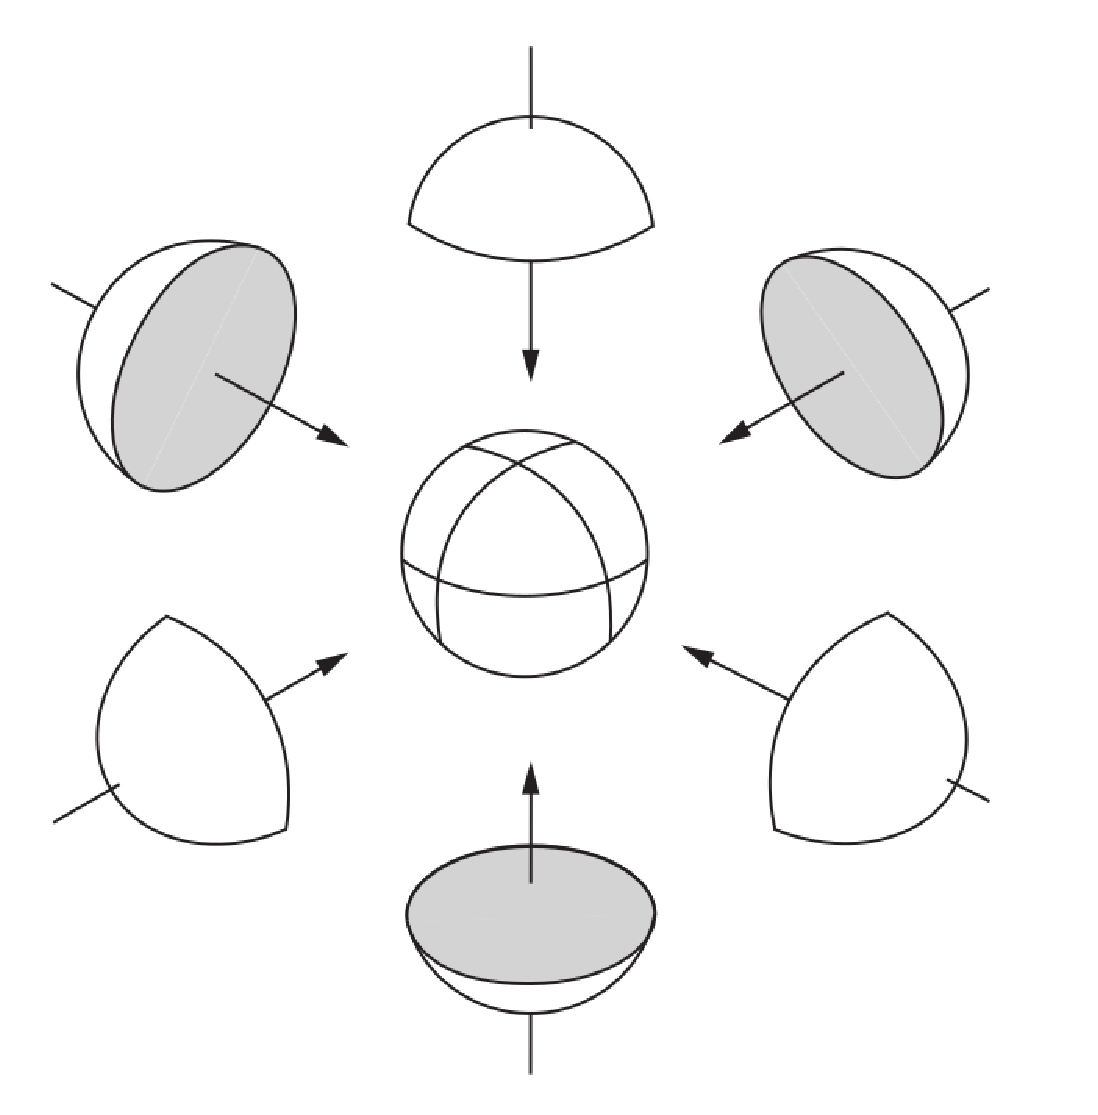
\includegraphics[scale=0.3]{eps/esfera}
		\caption{La esfera es una superficie.}
		\label{fig:esfera}
	\end{figure}
\end{example}

\begin{example}
	\label{exa:cilindro_recto}
	\index{Cilindro}
	Sea $S=\{(x,y,z)\in\R^3:x^2+y^2=1\}$ el cilindro recto de radio uno. Para
	demostrar que $S$ es una superficie consideramos la función
	$X\colon\R^2\to\R^3$, $X(u,v)=(\cos u,\sin u,v)$. Como
	\[
		X(u+2\pi,v)=X(u,v)
	\]
	para todo $u,v\in\R$, necesitamos restringir el dominio a un abierto donde
	$X$ quede inyectiva. Si $U=(0,2\pi)\times\R$, entonces la restricción
	$X|_U$ es inyectiva. El problema es que $X|_U$ no cubre a todo $S$ ya que
	la recta $(x,y,z)=(1,0,0)+z(0,0,1)$ no está contenida en $X(U)$. Necesitamos
	entonces otra carta y para esto podemos considerar la restricción $X|_V$, donde
	$V=(-\pi,\pi)\times\R$. Las parametrizaciones $X|_U$ y $X|_V$ cubren
	completamente a $S$. Un cálculo sencillo muestra que $S$ es entonces una
	superficie.
	\begin{figure}
		\centering
    	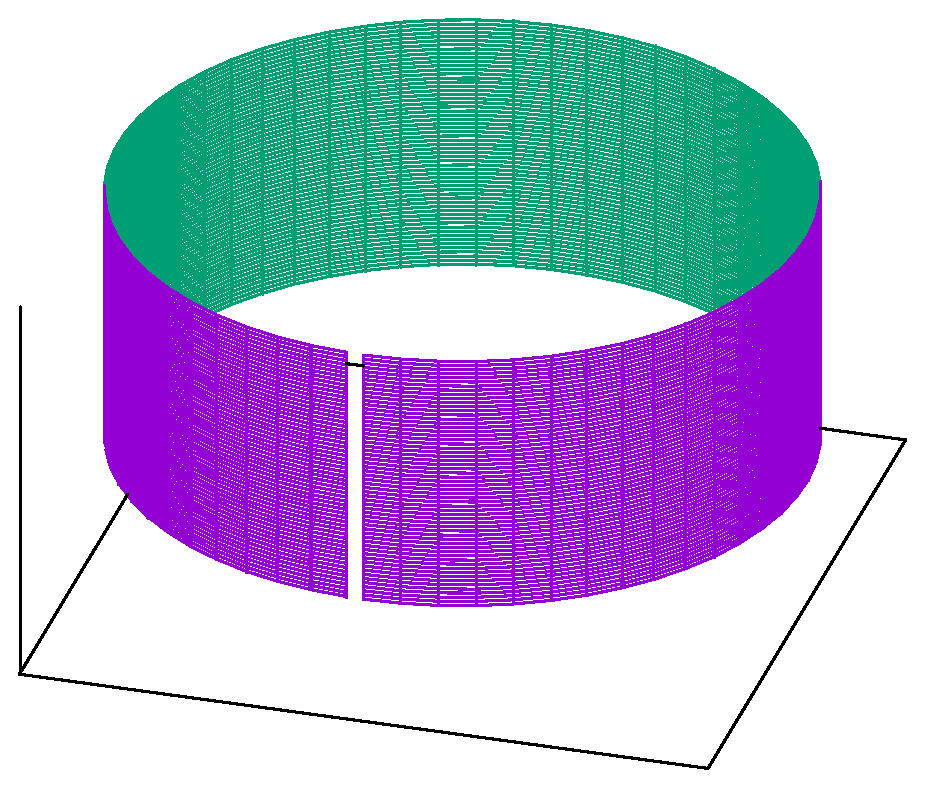
\includegraphics[scale=0.3]{eps/cilindro}
		\caption{Una de las parametrizaciones del cilindro recto.}
		\label{fig:cilindro}
	\end{figure}
\end{example}

Los gráficos de funciones diferenciables son superficies. La importancia de
este resultado radica en que nos permitirá construir muchas superficies.
Probaremos más adelante que toda superficie puede describirse localmente como
el gráfico de una función diferenciable. 

\begin{proposition}
	\index{Gráfico!de una función}
	Sea $U$ un abierto de $\R^2$ y sea $f\colon U\to\R$ una función
	$C^{\infty}$. El gráfico de $f$,
	\[
		G(f)=\{(u,v,f(u,v)):(u,v)\in U\}, 
	\]
	es una superficie regular.
\end{proposition}

\begin{proof}
	Sea $X\colon U\to\R^3$, $X(u,v)=(u,v,f(u,v))$. Como $f$ es $C^{\infty}$,
	$X$ es también $C^{\infty}$. Además $X$ es inyectiva y $X\colon U\to X(U)$
	es sobreyectiva, por lo que entonces existe $X^{-1}\colon X(U)\to U$. La
	función $X^{-1}$ es continua pues es la restricción a $G(f)$ de la
	función $(x,y,z)\mapsto (x,y)$.  Como los vectores $X_u=(1,0,f_u)$ y
	$X_v=(0,1,f_v)$ son linealmente independientes, se concluye que $G(f)$ es
	una superficie.
\end{proof}

Veamos un conjunto que no es una superficie: 

\begin{example}
	\index{Cono}
	Veamos que el cono circular 
	\[
		S=\{(x,y,z)\in\R^3:x^2+y^2=z^2\}
	\]
	no es una superficie. Observemos que $S\setminus\{(0,0,0)\}$ es unión
	disjunta de los conos $S_+=S\cap\{(x,y,z)\in\R^3:z>0\}$ y
	$S_-=S\cap\{(x,y,z)\in\R^3:z<0\}$. 
	
	Si fuera una superficie, tendríamos una parametrización $X\colon U\to\R^3$
	alrededor de punto $(0,0,0)\in S$. Sin pérdida de generalidad podemos
	suponer que $U$ es una bola con centro en un cierto punto $u\in U$ tal que
	$X(u)=(0,0,0)$. Como $X(U)=V\cap S$ para algún abierto $V$ de $\R^3$,
	existen puntos $p\in S_+\cap V$ y $q\in S_-\cap V$. Sean $a,b\in U$ tales
	que $X(a)=p$ y $X(b)=q$. En $U$ existe una curva continua que no contiene
	al punto $u$ y que une $a$ y $b$, digamos $\gamma\colon [0,1]\to U$ es tal
	que $u\not\in\gamma([0,1])$, $\gamma(0)=a$ y $\gamma(1)=b$. La composición
	$X\circ\gamma$ es entonces una curva continua en $S$ que une los puntos $p$
	y $q$ y que no pasa por $(0,0,0)$, una contradicción.

	Puede demostrarse que el conjunto $S\setminus\{(0,0,0)\}$ sí es una
	superficie que puede cubrirse con las parametrizaciones
	\[
		X_{\pm}\colon\R^2\setminus\{(0,0)\}\to\R^3,\quad
		X_{\pm}(u,v)=(u,v,\pm\sqrt{u^2+v^2}).
	\]

	\begin{figure}
		\centering
    	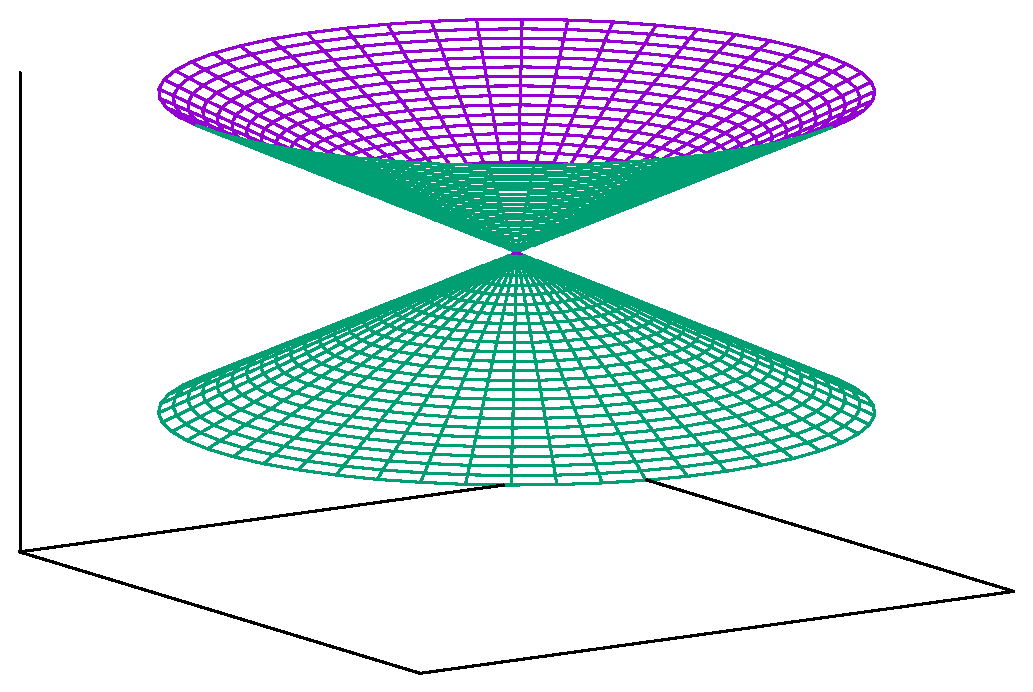
\includegraphics[scale=0.3]{eps/cono}
		\caption{El cono circular no es una superficie.}
		\label{fig:cono}
	\end{figure}
\end{example}

\begin{example}
	Si $S$ es una superficie y $T\subseteq S$ es un abierto no vacío, entonces
	$T$ es una superficie. De hecho, si $X\colon U\to X(U)$ es una
	parametrización de $S$ tal que $X(U)\cap T\ne\emptyset$, entonces $X\colon
	X^{-1}(T)\to T$ es una parametrización de $T$.
\end{example}

\chapter{El teorema de la función inversa}

\index{Teorema!de la función inversa}
En esta sección veremos algunos resultados levemente técnicos pero de gran
utilidad. Todos se basan en utilizar astutamente el \textbf{teorema de la
función inversa}:
\begin{quote}
	Sea $U$ un abierto de $\R^n$ y sea $f=(f_1,\dots,f_n)\colon U\to\R^n$ una
	función diferenciable. Sea $a\in U$ tal que la matriz jacobiana
	\[
		\frac{\partial f_i}{\partial u_j}(a)
	\]
	es inversible. Existe entonces un entorno $V$ de $a$ en $U$ y un entorno $W$
	de $f(a)$ en $\R^n$ tal que $f\colon V\to W$ tiene inversa diferenciable
	$f^{-1}\colon W\to V$. 
\end{quote}

Para la demostración referimos por ejemplo al capítulo dos del libro de
Spivak~\cite{MR0209411}, más precisamente al teorema 2--11 de la página 35. Es
importante mencionar que ahí el teorema está demostrado para funciones de clase
$C^1$. Sin embargo, la regla de Cramer y la fórmula para la diferencial de
$f^{-1}$ demuestran que $f^{-1}$ es de clase $C^\infty$ si $f$ lo es.

\begin{lemma}
	\label{lem:inverse}
	Sea $S$ una superficie y $X\colon U\to X(U)$ una parametrización alrededor
	de un punto $p\in S$. Existe entonces un entorno $M$ de $X^{-1}(p)$ y una
	proyección $\pi\colon \R^3\to\R^2$ en alguno de los planos coordenados de
	$\R^3$ tal que \[
	\pi\circ X\colon M\to (\pi\circ X)(M)
	\]
	es un difeomorfismo.
\end{lemma}

\begin{proof}
	Sea $q=X^{-1}(p)$. 
	Escribimos
	\[
		X(u,v)=(x(u,v),y(u,v),z(u,v)).
	\]
	Como $(dX)_q$ tiene rango dos, dos filas de $(dX)_q$ son linealmente
	independientes. Podemos suponer entonces sin pérdida de generalidad que 
	\[
	\det\begin{pmatrix}
			x_u(q) & x_v(q)\\
			y_u(q) & y_v(q)
		\end{pmatrix}\ne0.
	\]
	Sea $\pi\colon\R^3\to\R$, $\pi(x,y,z)=(x,y)$. Entonces $\pi\circ X\colon U\to\R^3$ es diferenciable
	y 
	\[
		d(\pi\circ X)_q=\begin{pmatrix}
			x_u(q) & x_v(q)\\
			y_u(q) & y_v(q)
		\end{pmatrix}
	\]
	es inversible. Por el teorema de la función inversa existe un entorno
	$M\subseteq U$ de $q$ tal que $\pi\circ X\colon M\to (\pi\circ X)(M)$ es un
	difeomorfismo.
\end{proof}

\begin{proposition}
	\index{Cambio de coordenadas}
	\label{pro:cambio_de_coordenadas}
	Si $S$ es una superficie, $p\in S$ y $X\colon U\to X(U)$ e $Y\colon V\to
	Y(V)$ son parametrizaciones de $S$ tales que $p\in X(U)\cap Y(V)=W$,
	entonces la función de cambio de coordenadas $X^{-1}\circ Y\colon
	Y^{-1}(W)\to X^{-1}(W)$ es un difeomorfismo (es decir: diferenciable, inversible y con inversa
	diferenciable).  
\end{proposition}

\begin{proof}
	Como $X$ e $Y$ son inversibles, basta con demostrar que $h=X^{-1}\circ Y$ es diferenciable. 
	Sean $r$ y $s$ tales que $p=X(r)=Y(s)$. El lema anterior
	nos dice que existe un entorno $M\subseteq X^{-1}(W)$ de $r$ y una proyección $\pi$, que podemos suponer 
	igual a $\pi(x,y,z)=(x,y)$, tal que $\pi\circ X\colon M\to (\pi\circ X)(M)$ es un difeomorfismo. Como $h^{-1}(M)$ es un entorno de $s$, 
	y además 
	\[
		(\pi\circ X)\circ h=(\pi\circ X)\circ (X^{-1}\circ Y)=\pi\circ Y
	\]
	en $h^{-1}(M)$, la función $h=(\pi\circ X)^{-1}\circ (\pi\circ Y)$ es
	diferenciable en $h^{-1}(M)$ (pues $(\pi\circ X)^{-1}\colon (\pi\circ
	X)(M)\to M$, $\pi\colon\R^3\to\R^2$ y $Y\colon h^{-1}(M)\to\R^3$ son
	funciones diferenciables).
%	Como $X$ e $Y$ son inversibles, basta con demostrar que $X^{-1}\circ Y$ es diferenciable. 
%	Escribimos
%	\[
%		X(u,v)=(x(u,v),y(u,v),z(u,v))
%	\]
%	y supongamos que 
%	\[
%		\det\begin{pmatrix}
%			x_u(q) & x_v(q)\\
%			y_u(q) & y_v(q)
%		\end{pmatrix}\ne0
%	\]
%	Sean $r\in
%	Y^{-1}(W)$ y $q=X^{-1}(Y(r))$. Sea 
%	\[
%		F\colon U\times\R\to\R^3,\quad
%		(u,v,t)\mapsto (x(u,v),y(u,v),z(u,v)+t).
%	\]
%	Entonces $F$ es $C^{\infty}$ y además la restricción $F|_{U\times\{0\}}=X$. Como
%	\[
%		\det (dF)_q=\det\begin{pmatrix}
%			x_u & x_v & 0\\
%			y_u & y_v & 0\\
%			z_u & z_v & 1
%		\end{pmatrix}
%		=\det\begin{pmatrix}
%			x_u(q) & x_v(q)\\
%			y_u(q) & y_v(q)
%		\end{pmatrix}\ne0,
%	\]
%	el teorema de la función inversa implica que existe un abierto $M$ de
%	$\R^3$ tal que $X(q)\in M$ donde existe $F^{-1}$ y es $C^{\infty}$. Como
%	$Y$ es continua, existe un abierto $N$ con $r\in N\subseteq V$ tal que
%	$Y(N)\subseteq M$ y donde la restricción $F^{-1}\circ Y|_N=(X^{-1}\circ
%	Y)|_N$ es $C^{\infty}$. Luego $X^{-1}\circ Y$ es diferenciable en
%	$Y^{-1}(W)$.
\end{proof}


Como consecuencia casi inmediata del lema~\ref{lem:inverse} obtenemos que
toda superficie es localmente una superficie de alguna de los siguientes tipos: 
$x=f(y,z)$, $y=g(x,z)$, $z=h(x,y)$. 

\begin{proposition}
	Sea $S$ una superficie regular y sea $p\in S$. Existe entonces un entorno
	$W$ de $p$ donde $S\cap W$ es el gráfico de una función diferenciable.
\end{proposition}

\begin{proof}
	Sea $X\colon U\to\R^3$, $X(u,v)=(x(u,v),y(u,v),z(u,v))$, una
	parametrización alrededor de $p$. Por el lema, existe un entorno $M$ de $X^{-1}(p)$ y una proyección
	$\pi\colon\R^3\to\R^2$ tal que $\pi\circ X\colon M\to (\pi\circ X)(M)$ es un difeomorfismo. Sin pérdida
	de generalidad podemos suponer que $\pi(x,y,z)=(x,y)$. Si escribimos
	\[
		X(u,v)=(x(u,v),y(u,v),z(u,v)
	\]
	y $f=\pi\circ X$, entonces $f(u,v)=(x(u,v),y(u,v))$. Como $f(M)=(\pi\circ
	X)(M)$ es un abierto de $\R^3$ y $f\colon M\to f(M)$ es un difeomorfismo, la función
	$h\colon f(M)\to\R$, $h(x,y)=z\circ f^{-1}(x,y)$, es diferenciable y 
	\[
		X(M)=X\circ f^{-1}(f(M))=\{(x,y,h(x,y)):(x,y)\in f(M)\}
	\]
	es el gráfico de la función $h$. 
%	matriz de $dX_p$ tiene rango dos, algún menor tiene determinante distinto
%	de cero, digamos
%	\[
%		\frac{\partial(x,y)}{\partial(u,v)}(u_0,v_0)=\det\begin{pmatrix}
%			x_u & x_v\\
%			y_u & y_v
%		\end{pmatrix}(u_0,v_0)\ne0.
%	\]
%	Por el teorema de la función inversa existe un entorno $V\subseteq U$ de
%	$(u_0,v_0)$ tal que 
%	\[
%		f\colon V\to f(V),\quad 
%		f(u,v)=(x(u,v),y(u,v)),
%	\]
%	es un difeomorfismo. Como $f(V)$ es un abierto de $\R^2$ y la función
%	$h\colon f(V)\to\R$, $h(x,y)=z\circ f^{-1}(x,y)$, es diferenciable, tenemos
%	en consecuencia que 
%	\[
%		W=X(V)=X\circ f^{-1}(f(V))=\{(x,y,h(x,y)):(x,y)\in f(V)\}
%	\]
%	es el gráfico de la función $h$.

%	Sea $X\colon U\to\R^3$, $X(u,v)=(x(u,v),y(u,v),z(u,v))$, una
%	parametrización alrededor de $p$ y supongamos que $X(u_0,v_0)=p$. Como la
%	matriz de $dX_p$ tiene rango dos, algún menor tiene determinante distinto
%	de cero, digamos
%	\[
%		\frac{\partial(x,y)}{\partial(u,v)}(u_0,v_0)=\det\begin{pmatrix}
%			x_u & x_v\\
%			y_u & y_v
%		\end{pmatrix}(u_0,v_0)\ne0.
%	\]
%	Por el teorema de la función inversa existe un entorno $V\subseteq U$ de
%	$(u_0,v_0)$ tal que 
%	\[
%		f\colon V\to f(V),\quad 
%		f(u,v)=(x(u,v),y(u,v)),
%	\]
%	es un difeomorfismo. Como $f(V)$ es un abierto de $\R^2$ y la función
%	$h\colon f(V)\to\R$, $h(x,y)=z\circ f^{-1}(x,y)$, es diferenciable, tenemos
%	en consecuencia que 
%	\[
%		W=X(V)=X\circ f^{-1}(f(V))=\{(x,y,h(x,y)):(x,y)\in f(V)\}
%	\]
%	es el gráfico de la función $h$.
\end{proof}

\begin{example}
	El cono $C=\{(x,y,z)\in\R^3:z=\sqrt{x^2+y^2}\}$ no es una superficie. Por
	la proposición anterior sabemos que alrededor del origen, $C$ es el gráfico
	de una función diferenciable. Las posibilidades son: $x=f(y,z)$,
	$y=g(x,z)$, $z=h(x,y)$. Como las proyecciones de $C$ sobre $y=0$ y $x=0$ no
	son inyectivas, se concluye que alrededor del origen $C$ es el gráfico de
	la función $z=\sqrt{x^2+y^2}$, que no es una función diferenciable. 
\end{example}

Recordemos que si $f\colon\R^n\to\R$ es una función y $a\in\R$, 
\[
	f^{-1}(a)=\{p\in\R^n:f(p)=a\}.
\]

\begin{definition}
	\index{Valor regular}
	Sea $U$ un abierto de $\R^3$ y sea $f\colon U\to\R$ una función
	diferenciable. Diremos que $a\in\R$ es un \textbf{valor regular} de $f$ si
	para cada $p\in f^{-1}(a)$ se tiene $\nabla f(p)\ne 0$.
\end{definition}

La siguiente proposición permite construir muy fácilmente muchas superficies.

\begin{proposition}
	\label{pro:regular}
	Sea $f\colon U\to\R$ una función diferenciable.  Si $0$ es un valor regular
	para $f$ y además $S=f^{-1}(0)$ es no vacío, entonces $S$ es una superficie.
\end{proposition}

\begin{proof}
	Sea $p=(x_0,y_0,z_0)$ tal que $f(p)=0$ y $f_z(p)\ne 0$. Sea $F\colon
	U\to\R^3$ la función dada por $F(x,y,z)=(x,y,f(x,y,z))$. Como el jacobiano
	de $F$ en $p$ es 
	\[
		\det\begin{pmatrix}
			1 & 0 & 0\\
			0 & 1 & 0\\
			f_x(p) & f_y(p) & f_z(p)
		\end{pmatrix}
		=f_z(p)\ne 0,
	\]
	el teorema de la función inversa implica que existen entornos $V\subseteq U$ de $p$ y
	$W$ de 
	\[
		F(p)=(x_0,y_0,f(x_0,y_0,z_0))=(x_0,y_0,0) 
	\]
	tales que $F\colon V\to W$ es un inversible con inversa diferenciable
	$G\colon W\to U$. Como $G$ es la inversa de $F$, podemos escribir $G(x,y,z)=(x,y,g(x,y,z))$ para alguna función diferenciable $g$. 
	Observemos que como 
	\[
		f(x,y,z)=0\Longleftrightarrow
		F(x,y,z)=(x,y,0)\Longleftrightarrow
		(x,y,z)=G(x,y,0)\Longleftrightarrow
		z=g(x,y,0),
	\]
	el conjunto $V\cap f^{-1}(0)$ es el gráfico de la función diferenciable
	$h(x,y)=g(x,y,0)$ con dominio $\{(x,y)\in\R^2:(x,y,0)\in W\}$. Luego
	$f^{-1}(0)$ es una superficie.
\end{proof}

Como aplicación de la proposición anterior veamos que los elipsoides (y en
particular las esferas) son superficies: 

\begin{example}
	El elipsoide $S$ dado por los puntos $(x,y,z)\in\R^3$ tales que 
	\[
		\frac{x^2}{a^2}+\frac{y^2}{b^2}+\frac{z^2}{c^2}=1
	\]
	es una superficie
	pues $0$ es un valor regular para la función
	\[
		f(x,y,z)=\frac{x^2}{a^2}+\frac{y^2}{b^2}+\frac{z^2}{c^2}-1. 
	\]
%	Es evidente que $f$
%	es diferenciable. Además $0$ es un valor regular de $f$ pues 
%	\[
%		\nabla f(x,y,z)=\left(\frac{2x}{a^2},\frac{2y}{b^2},\frac{2z}{c^2}\right)=(0,0,0) 
%	\]
%	si y sólo si $(x,y,z)=(0,0,0)$. Como $(0,0,0)\not\in f^{-1}(\{0\})$, la
%	proposición~\ref{pro:regular} muestra que $S$ sea una superficie. 
\end{example}

Veamos ahora un ejemplo de superficie no conexa:

\begin{example}
	El hiperboloide de dos hojas
	\[
		S=\{(x,y,z)\in\R^3:-x^2-y^2+z^2=1\}
	\]
	es una superficie pues $0$ es un valor regular para la función 
	\[
		f(x,y,z)=-x^2-y^2+z^2-1.
	\]
\end{example}

Preimagen de valores no regulares también podrían ser superficies:

\begin{example}
	Si $f(x,y,z)=z^2$, entonces $0$ no es un valor regular para $f$. Sin
	embargo, el conjunto $f^{-1}(0)$ es una superficie pues
	$f^{-1}(0)=\{(x,y,z)\in\R^3:z=0\}$.
\end{example}

%\begin{example}[cuádricas]
%	Sea $A\in\R^{4\times 4}$ una matriz simétrica y sea $f\colon\R^3\to\R$,
%	$f(v)=(1,v^T)A\colvec{2}{1}{v}$.  Definimos $S=f^{-1}(\{0\})$ y nos
%	preguntamos si $0$ es un valor regular para $f$. 
%
%	Para $v\in f^{-1}(\{0\})$ y $w\in\R^3$ calculemos $(df)_v(w)$. Sea $\alpha$
%	una curva tal que $\alpha(0)=v$ y $\alpha'(0)=w$. 
%\end{example}
%
%\begin{example}[toro de revolución]
%	Sean $a,r\in\R$ tales que $a>r>0$. Vamos a construir una superficie $S$ al
%	hacer girar sobre el eje $z$ al círculo 
%	\[
%	S^1(r)\subseteq\{(x,y,z)\in\R^3:x=0\}
%	\]
%	de radio $r$ y con centro en el punto $(0,a,0)$. El círculo incial es
%	\[
%		\{(x,y,z)\in\R^3:z^2+(y-a)^2=r^2,\,x=0\}
%	\]
%	y luego
%	\[
%		S=\{(x,y,z)\in\R^3:(\sqrt{z^2+y^2}-a)^2+x^2=r^2\}.
%	\]
%	Sea $f$ la función definida sobre $\R^3$\framebox{completar}
%\end{example}

%Otra aplicación interesante del teorema de la función inversa es la siguiente:
%toda superficie es localmente el gráfico de una función diferenciable:

\chapter{El plano tangente y las funciones diferenciables}

Veamos ahora cómo trasportar los conceptos del cálculo diferencial clásico al
cálculo diferencial en superficies.  Comenzaremos con la definición de función
diferenciable. Para la definición de diferenciabilidad resultará esencial tener
a mano la proposición~\ref{pro:cambio_de_coordenadas}, que establece que los
cambios de coordenadas son funciones diferenciables.

\begin{definition}
	\label{def:diferenciable1}
	\index{Función!diferenciable}
	Una función $f\colon S\to T$ entre superficies se dirá
	\textbf{diferenciable} si para cada $p\in S$ existe una parametrización
	$X\colon U\to S$ alrededor de $p$ y existe una parametrización $Y\colon
	V\to T$ alrededor de $f(p)$ tal que la composición $Y^{-1}\circ f\circ X$
	es diferenciable.
\end{definition}

La definición anterior no incluye funciones a valores reales:

\begin{definition}
	Si $S$ es una superficie, 
	una función $f\colon S\to\R$ se dirá \textbf{diferenciable} si para cada $p\in S$ existe
	una parametrización $X\colon U\to S$ alrededor de $p$ tal que 
	$f\circ X$ es diferenciable.
\end{definition}

Las composiciones $f\circ X$ y $Y^{-1}\circ f\circ X$ de las definiciones
anteriores se conoce como las \textbf{expresiones en coordenadas} de la función
$f$.  Nuestras definiciones de diferenciabilidad no dependen de las
parametrizaciones elegidas. Lo demostraremos para el caso de funciones entre
superficies: como los cambios de coordenadas son funciones diferenciables, la
composición 
\[
	Y^{-1}\circ f\circ X=(Y^{-1}\circ\overline{Y})\circ (\overline{Y}^{-1}\circ f\circ\overline{X})\circ (\overline{X}^{-1}\circ X)
\]
es diferenciable por ser composición de funciones diferenciables.

%Si $S$ es una superficie y $f\colon S\to\R^3$ es una función tal que
%$f(S)\subseteq T$ para alguna superficie $T$, escribiremos $f\colon S\to T$.
%Entonces $f\colon S\to T$ es diferenciable si para existe una
%parametrización $X\colon U\subseteq\R^2\to S$ de $S$ tal que la composición 
%\[
%f\circ X\colon U\to T\hookrightarrow\R^3
%\]
%es diferenciable.

%\begin{definition}
%	\label{def:diferenciable3}
%	\index{Función!diferenciable}
%	Sean $S$ y $T$ superficies. Diremos que una función $f\colon S\to T$ es
%	\textbf{diferenciable} si para toda parametrización $X\colon
%	U\subseteq\R^2\to S$ de $S$, la composición 
%	\[
%		f\circ X\colon U\to S\hookrightarrow\R^3
%	\]
%	es diferenciable.
%\end{definition}

De la definición se obtiene fácilmente que toda función diferenciable es
continua. Por ejemplo: como $Y^{-1}\circ f\circ X\colon U\to\R^3$ es continua por ser diferenciable, 
se concluye que $f=Y\circ (Y^{-1}\circ f\circ X)\circ X^{-1}$ es también una
función continua.

\begin{example}
	Sea $V\subseteq\R^3$ un abierto y sea $F\colon V\to\R$ una función
	diferenciable. Si $S$ es una superficie contenida en $V$, la restricción
	$F|_S\colon S\to\R$ es una función diferenciable pues si $X\colon U\to
	X(U)\subseteq V$ es una parametrización, la composición 
	\[
		(F|_S)\circ X=F|_{X(U)}
	\]
	es diferenciable. 
\end{example}

El ejemplo anterior tiene varias consecuencias útiles e interesantes:

%El ejemplo anterior implica que si $S$ es una superficie, la inclusión
%$S\hookrightarrow\R^3$ y la identidad $S\to S$ son funciones diferenciables.
%También implica que la función \textbf{altura} es diferenciable:
%
\begin{example}
	\index{Función!altura}
	Sea $P\subseteq\R^3$ un plano con vector normal $n$ y sea $p_0\in P$. Si
	$S$ es una superficie, la función $h\colon S\to\R^3$, $p\mapsto\langle
	p-p_0,n\rangle$, es diferenciable pues es la restricción de la función
	$\R^3\to\R$, $p\mapsto \langle p-p_0,n\rangle$.
\end{example}

\begin{example}
	\index{Función!distancia al cuadrado}
	Sea $p_0\in\R^3$.  La función $f\colon S\to\R$, $f(p)=\|p-p_0\|^2$, es
	diferenciable. 
\end{example}

\begin{example}
	\index{Inclusión}
	Las componentes de la inclusión $\iota=(\iota_1,\iota_2,\iota_3)\colon
	S\to\R^3$ son funciones diferenciables. Por ejemplo: como $\pi_1\colon
	\R^3\to\R$, $(x,y,z)\mapsto x$, es diferenciable, la restricción
	$\pi_1|_S=\iota_1$ es también diferenciable. 
\end{example}

\index{Difeomorfismo}
Una función diferenciable $f\colon S\to T$ entre superficies es un
\textbf{difeomorfismo} si es inversible y su inversa es diferenciable.  La
diferenciabilidad de los cambios de coordenadas implica que las
parametrizaciones son difeomorfismos.

\begin{example}
	Si $X\colon U\to X(U)$ es una parametrización de una superficie, entonces
	$X^{-1}\colon X(U)\to U$ es diferenciable pues si $Y\colon V\to Y(V)$ es
	una parametrización tal que $W=X(U)\cap Y(V)\ne\emptyset$, entonces
	\[
		Y^{-1}\circ X\colon X^{-1}(W)\to Y^{-1}(W)
	\]
	es diferenciable.
\end{example}

\begin{example}
	Sean $T$ una superficie, $V\subseteq\R^3$ un abierto y $F\colon V\to T$ una
	función diferenciable. Si $S$ es una superficie contenida en $V$, la
	restricción $F|_S\colon S\to T$ es una función diferenciable. Si $X\colon
	U\to X(U)\subseteq V$ e $Y\colon V\to T$ son parametrizaciones tales que
	$F(X(U))\subseteq Y(V)$, la composición 
	\[
		Y^{-1}\circ (F|_S)\circ X=Y^{-1}\circ F|_{X(U)}
	\]
	es diferenciable. 
\end{example}

Veamos algunos casos particulares del ejemplo anterior:

\begin{example}
	Sean $a,b,c\in\R$ no nulos. Como 
	\[
		F\colon\R^3\to\R^3,\quad
		F(x,y,z)=(ax,by,cz),
	\]
	es diferenciable, la restricción $F|_{S^2}$ de $F$ a
	la esfera unitaria es una función diferenciable 
	\[
		S^2\to\left\{(x,y,z)\in\R^3:\frac{x^2}{a^2}+\frac{y^2}{b^2}+\frac{z^2}{c^2}=1\right\}
	\]
\end{example}

\begin{example}
	\index{Curva!en una superficie}
	Si $\alpha\colon I\to\R^3$ es una curva tal que $\alpha(I)$ está contenida
	en una superficie $S$, entonces $\alpha\colon I\to S$ es diferenciable.
\end{example}

El ejemplo anterior nos permite hablar de curvas (diferenciables) en
superficies. Esto resulta fundamental para poder definir el plano tangente a una superficie
sin apelar a parametrizaciones:
%
%El siguiente lema será de gran utilidad y nos sirve para entender
%cómo funcionan las definiciones que vimos hasta ahora.
%
%\begin{lemma}
%	Sea $X\colon U\to S$ una parametrización de una superficie $S$. Si
%	$\alpha\colon I\to S$ es una curva cuya imagen está contenida $X(U)$,
%	entonces existen únicas funciones diferenciables $a$ y $b$ tales que 
%	$\alpha(t)=X(a(t),b(t))$ 
%	para todo $t$.
%\end{lemma}
%
%\begin{proof}
%	La función $X^{-1}\circ\alpha\colon I\to U$ es diferenciable. Si $a$ y $b$
%	son las funciones coordenadas euclidianas de $X^{-1}\circ\alpha$, entonces
%	$\alpha=X\circ X^{-1}\circ \alpha=X(a,b)$. Veamos ahora la unicidad: si $\alpha=X(c,d)$, entonces
%	\[
%		(a,b)=X^{-1}\circ\alpha=X^{-1}X(c,d)=(c,d).\qedhere
%	\]
%\end{proof}

%\begin{exercise}
%	Sea $S$ una superficie y sea $p_0\in\R^3$. 
%	Demuestre que la función
%	\[
%		S\to\R,\quad
%		p\mapsto\|p-p_0\|^2,
%	\]
%	es diferenciable.
%\end{exercise}

\begin{definition}
	\index{Vector!tangente a una superficie}
	Sea $S$ una superficie y sea $p\in S$. Decimos que $v\in\R^3$ es
	un \textbf{vector tangente} a $S$ en $p$ si existe una curva
	$\alpha\colon(-\epsilon,\epsilon)\to S$ tal que $\alpha(0)=p$ y
	$\alpha'(0)=v$. 
\end{definition}

Escribiremos $T_pS$ para denotar al conjunto de los vectores tangente a la
superficie $S$ en el punto $p$. Esta definición, si bien no depende del uso de
coordenadas, no es conveniente para hacer cálculos.  Para poder calcular planos
tangente tenemos el siguiente resultado:

\begin{proposition}
	Sea $S$ una superficie y sea $p\in S$. Si $X\colon 	U\to S$ es una
	parametrización de $S$ en $p$, entonces
	\[
		T_pS=(dX)_{X^{-1}(p)}(\R^2).
	\]
\end{proposition}

\begin{proof}
	Sea $v\in T_pS$ y sea $\alpha\colon(-\epsilon,\epsilon)\to S$ una curva tal que
	$\alpha(0)=p$ y $\alpha'(0)=v$. Sin pérdida de generalidad podemos suponer
	que $\alpha(-\epsilon,\epsilon)\subseteq X(U)$. Si 
	\[
		\beta=X^{-1}\circ\alpha\colon (-\epsilon,\epsilon)\to U,
	\]
	entonces $\beta$ es diferenciable y tal que $\beta(0)=X^{-1}(p)$. Al
	derivar $\alpha=X\circ\beta$ y usar la regla de la cadena se
	conluye entonces que 
	\[
		v=\alpha'(0)=dX_{X^{-1}(p)}(\beta'(0)).
	\]

	Sea $w\in\R^2$ y sea $\beta(t)=X^{-1}(p)+tw$. Sea $\epsilon>0$ tal que
	$\beta(t)\subseteq U$ si $|t|<\epsilon$. Al derivar $X\circ\beta=\alpha$
	obtenemos, gracias a la regla de la cadena, que 
	\[
		dX_{X^{-1}(p)}(w)=dX_{X^{-1}(p)}(\beta'(0))=\alpha'(0)\in T_pS.\qedhere
	\]
\end{proof}

La proposición anterior nos dice que si $S$ es una superficie y $p\in S$, entonces
$T_pS$ es un espacio vectorial. Tenemos entonces la siguiente consecuencia: 

\begin{proposition}
	Sea $S$ una superficie y sea $p\in S$. 
	Si $X\colon U\to X(U)$ es una parametrización de $S$
	en $p$ y $q=X^{-1}(p)$, entonces $T_pS$ está generado por
	$\{X_u(q),X_v(q)\}$. 
\end{proposition}

\begin{proof}
	Gracias a la proposición anterior, basta con demostrar que el espacio generado por
	$X_u(q)$ y $X_v(q)$ está contenido en $T_pS$.  Sea
	$v=aX_u(q)+bX_v(q)$. Entonces  la curva $\alpha(t)=X(q+(a,b)t)$ cumple que $\alpha(0)=p$ y
	$\alpha'(0)=v$. 
\end{proof}

Calculemos algunos planos tangente:

\begin{example}
	\label{exa:TpS:z=x^2+y^2} 
	\index{Paraboloide!elíptico}
	Calculemos el plano tangente a la superficie $z=x^2+y^2$ en el punto $p=(1,1,2)$. Consideramos
	la parametrización $X(u,v)=(u,v,u^2+v^2)$, $p=X(1,1)$. Calculamos:
	\[
		X_u(u,v)=(1,0,2u),\quad
		X_v(u,v)=(0,1,2v).
	\]
	El plano tangente $T_pS$ es el plano de ecuación $z=2(x+y)$ pues $T_pS$
	está entonces generado por $X_u(1,1)=(1,0,2)$ y $X_v(1,1)=(0,1,2)$. 
\end{example}

\begin{example}
	Sea $P$ algún plano con normal $(a,b,c)\in\R^3$, digamos
	\[
		P=\{(x,y,z)\in\R^3:ax+by+cz=d\},
	\]
	donde $c\ne 0$, y sea 
	$p\in P$. Vamos a calcular $T_pP$. Vimos que
	\[
		X(u,v)=\left(u,v,(-a/c)u+(-b/c)v+d/c\right)
	\]
	es una parametrización aldededor de $p\in P$. Por la proposición anterior
	sabemos que $T_pP$ es el espacio vectorial de dimensión dos generado por
	$X_u=(1,0,-a/c)$ y $X_v=(0,1,-b/c)$. Como 
	\[
		X_u\times X_v=(ac,cb,c^2),
	\]
	se concluye que $(a,b,c)$ es el normal al plano $T_pP$. 
\end{example}

Vimos que la preimagen de valor regular da una superficie. Calculemos el plano
tangente de este tipo de superficies:

\begin{proposition}
	Sea $f\colon\R^3\to\R$ una función diferenciable tal que $0$ es un valor regular.
	Si $S=f^{-1}(0)$ y $p\in S$, entonces 
	\[
		T_pS=\ker((df)_p\colon\R^3\to\R).
	\]
\end{proposition}

\begin{proof}
	Como $0$ es un valor regular, 
	\[
		\dim T_pS=\dim\ker((df)_p\colon\R^3\to\R)=2.
	\]
	Basta entonces con demostrar que $T_pS\subseteq\ker( (df)_p\colon\R^3\to\R)$.
	Sea $v\in T_pS$ y sea $\alpha\colon(-\epsilon,\epsilon)\to S$ tal que
	$\alpha(0)=p$ y $\alpha'(0)=v$. Como $f(\alpha(t))=0$ para todo $t$, al
	derivar y usar la regla de la cadena, 
	\[
		0=\frac{d}{dt}(f\circ\alpha)(0)=(df)_{\alpha(0)}\alpha'(0)=(df)_p(v).
	\]
\end{proof}

\begin{example}
	Sea $S^2=\{p\in\R^3:\|p\|^2=1\}$ la esfera de radio uno y centro en el
	origen. Sabemos que $S^2=f^{-1}(1)$, donde 
	\[
		f\colon\R^3\to\R,\quad
		f(p)=\|p\|^2=\langle p,p\rangle.
	\]
	Para calcular $T_pS^2$ en algún punto $p$ de $S^2$ podemos entonces
	utilizar el resultado del ejemplo anterior:
	\[
		T_pS^2=\ker(df_p\colon\R^3\to\R).		
	\]
	Si $v\in T_pS^2$ y $\alpha$ es una curva en $S^2$ tal que $\alpha(0)=p$ y $\alpha'(0)=v$, entonces 
	\[
		df_p(v)=\frac{d}{dt}(f(\alpha(t))(0)=2\langle v,p\rangle.
	\]
	Luego $T_pS^2=\{v\in\R^3:\langle v,p\rangle=0\}$ es el plano cuyo vector
	normal está en la dirección de $p$.
\end{example}

% cilindro

\begin{definition}
	\index{Diferencial}
	Sea $S$ una superficie y sea $f\colon S\to\R^n$ una función diferenciable.
	Para cada $p\in S$ se define la diferencial de $f$ en $p$ como la
	función
	\[
			(df)_p\colon T_pS\to\R^n,\quad
			(df)_p(v)=\frac{d}{dt}f(\alpha(t))(0)=(f\circ\alpha)'(0),
	\]
	donde $\alpha$ es una curva en $S$ tal que $\alpha(0)=p$ y $\alpha'(0)=v$.
\end{definition}

\begin{proposition}
	Sea $S$ una superficie y sea $p\in S$. Para cada $f\colon S\to\R^n$ 
	diferenciable, la diferencial $(df)_p$ está bien definida y es una
	transformación lineal. 
\end{proposition}

\begin{proof}
	Sea $X\colon U\to X(U)$ una parametrización en $p$ y sea $q=X^{-1}(p)$. Sea
	$v\in T_pS$ y sea $\alpha\colon(-\epsilon,\epsilon)\to S$ una curva tal que
	$\alpha(0)=p$ y $\alpha'(0)=v$. Sin pérdida de generalidad podemos suponer
	que $\alpha(-\epsilon,\epsilon)\subseteq X(U)$. Como $X\circ (X^{-1}\circ
	\alpha)=\alpha$, al derivar y evaluar en $t=0$, obtenemos
	\[
		(dX)_q(X^{-1}\circ\alpha)'(0)=v,
	\]
	que podemos reescribir como
	\[
		(X^{-1}\circ\alpha)'(0)=(dX_q)^{-1}(v).
	\]
	Al calcular 
	\begin{align*}
		(df)_p(v) &= (f\circ\alpha)'(0)
		=\frac{d}{dt}\left( (f\circ X)\circ (X^{-1}\circ\alpha)\right)(0)\\
		&=d(f\circ X)_q(X^{-1}\circ\alpha)'(0)
		=d(f\circ X)_q(dX_q)^{-1}(v),
	\end{align*}
	vemos que $(df)_p$ está bien definida (no depende de la curva $\alpha$ que
	elegimos) y que es una transformación lineal por ser producto de
	transformaciones lineales.
\end{proof}

Para poder calcular efectivamente la diferencial de una función contamos con la
siguiente herramienta:

\begin{lemma}
	Sea $X\colon U\to S$ una parametrización de una superficie $S$ alrededor de un punto $p=X(u_0,v_0)$. 
	Si $f\colon S\to\R^3$ es una función diferenciable, entonces
	\begin{align}
		\label{eq:dfXu}&(df)_p(X_u(u_0,v_0))=(f\circ X)_u(u_0,v_0),\\
		\label{eq:dfXv}&(df)_p(X_v(u_0,v_0))=(f\circ X)_v(u_0,v_0).
	\end{align}
\end{lemma}

\begin{proof}
	Demostremos~\eqref{eq:dfXu}. Si $\alpha(t)=X(u_0+t,v_0)$, entonces
	$\alpha(0)=p$ y $\alpha'(0)=X_u(u_0,v_0)$. Calculamos:
	\[
		(df)_p(X_u(u_0,v_0))=\frac{d}{dt}(f\circ\alpha)(0)=\frac{d}{dt}\bigg|_{t=0}(f\circ X)(u_0+t,v_0)=(f\circ X)_u(u_0,v_0).
	\]
	La igualdad~\eqref{eq:dfXv} se demuestra en forma similar.
	%al considerar la curva
	%$\beta(t)=X(u_0,v_0+t)$.
\end{proof}

\begin{example}
	\index{Paraboloide!elíptico}
	Sea $S$ la superficie dada por $z=x^2+y^2$. Sea $f\colon S\to\R^3$ la
	función dada por
	\[
		f(x,y,z)=(\cos(\pi z),xz,y+z^2).
	\]
	Queremos ver que $f$ es diferenciable y para $p=(1,1,2)$ calcular $(df)_p(2,-1,2)$ Si
	consideramos la parametrización $X(u,v)=(u,v,u^2+v^2)$, entonces
	\[
		f\circ X(u,v)=(\cos (\pi(u^2+v^2),u(u^2+v^2),v+(u^2+v^2)^2)
	\]
	y luego $f$ es diferenciable. 

	Vimos que en el ejemplo~\ref{exa:TpS:z=x^2+y^2} que
	$T_p=\langle (1,0,2),(0,1,2)\rangle$. Como 
	\[
		(2,-1,2)=2(1,0,2)+(-1)(0,1,2),
	\]
	necesitamos
	poder calcular $(df)_p(1,0,2)$ y $(df)_p(0,1,2)$. 
%	Como
%	\begin{align*}
%		&(df)_p(1,0,2)=(f\circ X)_u(1,1),
%		&&(df)_p(0,1,2)=(f\circ X)_v(1,1),
%	\end{align*}
	Calculamos
	\begin{align*}
	 &(f\circ X)_u(u,v)=(-2\pi u\sin(\pi(u^2+v^2)),3u^2+v^2,4u(u^2+v^2)),\\
	 &(f\circ X)_v(u,v)=(-2\pi v\sin(\pi(u^2+v^2)),2uv,1+4v(u^2+v^2)),
	\end{align*}
	y entonces 
	\begin{align*}
		&(df)_p(1,0,2)=(f\circ X)_u(1,1)=(0,4,8),\\
		&(df)_p(0,1,2)=(f\circ X)_v(1,1)=(0,2,9).
	\end{align*}
	Luego 
	\[
		(df)_p(2,-1,2)=2(0,4,8)-(0,2,9)=(0,6,7). 
	\]
\end{example}

En el ejemplo anterior podríamos haber utilizado otra parametrización, digamos
por ejemplo $Y(u,v)=(u,\sqrt{v-u^2},v)$, y obviamente obtendríamos también que
$(df)_p(2,-1,2)=(0,6,7)$. 

\begin{example}
	Sea $S$ una superficie y 
	sean $p_0\in\R^3$ y $a\in\R^3\setminus\{0\}$. Si  
	$h\colon S\to\R$, $h(p)=\langle p-p_0,a\rangle$, entonces
	$(dh)_p(v)=\langle v,a\rangle$ para todo $v\in T_pS$. 
\end{example}

\begin{example}
	Sea $S$ una superficie y 
	sea $p_0\in\R^3$. Si $f\colon S\to\R$, $f(p)=\|p-p_0\|^2$, entonces
	$(df)_p(v)=2\langle v,p-p_0\rangle$ para todo $v\in T_pS$. 
\end{example}

\begin{example}
	Sea $S$ una superficie. 
	y sea $\iota\colon S\to\R^3$ la inclusión canónica. Entonces
	$(d\iota)_p(v)=v$ 
	para todo $v\in T_pS$. 
\end{example}

\begin{theorem}[regla de la cadena]
	\index{Regla de la cadena}
	\label{thm:chain_rule} 
	Sean $f\colon S_1\to S_2$ y $g\colon S_2\to S_3$ funciones diferenciables
	entre superficies. Si $p\in S_1$, entonces $g\circ f$ es diferenciable y además 
	\[
		d(g\circ f)_p=(dg)_{f(p)}\circ (df)_p.
	\]
\end{theorem}

\begin{proof}
	Sean $X$ una parametrización de $S_1$ y $Z$ una parametrización de $S_3$. 
	La composición $Z^{-1}\circ (g\circ f)\circ X$ es diferenciable ya que puede escribirse como
	\[
		Z^{-1}\circ (g\circ f)\circ X=(Z^{-1}\circ g\circ Y)\circ (Y^{-1}\circ f\circ X),
	\]
	donde $Y$ es una parametrización de $S_2$.

	Sea $v\in T_pS_1$.  Si $\alpha$ una curva en $S_1$ tal que $\alpha(0)=p$ y
	$\alpha'(0)=v$, entonces $f\circ\alpha$ es una curva en $S_2$
	tal que $(f\circ\alpha)(0)=f(p)$ y $(f\circ\alpha)'(0)=(df)_p(v)$ por
	definición. Tenemos entonces que 
	\begin{align*}
		d(g\circ f)_p(v)&=((g\circ f)\circ\alpha)'(0)=(g\circ (f\circ\alpha)'(0)\\
		&=(dg)_{f(p)}(f\circ\alpha)'(0)=(dg)_{f(p)}\circ (df)_p(v).\qedhere
	\end{align*}
\end{proof}

\chapter{Orientabilidad}

Nuestro objetivo es poder medir cuánto se curva una superficie. Si en cada
punto $p$ de nuestra superficie se tiene bien definido un vector normal $N(p)$,
es natural estudiar la tasa de variación de $N(p)$. 

\index{Campo vectorial}
Recordemos algunas definiciones básicas.  Un \textbf{campo vectorial} $V$ en
una superficie $S$ es una función diferenciable $V\colon S\to\R^3$. El campo
$V$ se será \textbf{normal} si $\langle V(p), v\rangle$ para todo $v\in T_p$, y
se será \textbf{unitario} si $\langle V(p),V(p)\rangle=1$ para todo $p\in S$. 

\begin{definition}
	\index{Superficie!orientable}
	Diremos que una superficie $S$ es \textbf{orientable} si existe un campo
	vectorial $N\colon S\to\R^3$ normal y unitario.
\end{definition}

El siguiente lema muestra que toda superficie es localmente orientable:

\begin{lemma}
	Si $S$ es una superficie y $X\colon U\to S$ es una parametrización,
	entonces existe al menos un campo vectorial normal unitario en $X(U)$.
\end{lemma}

\begin{proof}
	Sea $q\in U$ y sea $p=X(q)$. Como $X_u(q)$ y $X_v(q)$ son linealmente
	independientes, el vector
	\[
		N_X(q)=\frac{X_u(q)\times X_v(q)}{\|X_u(q)\times X_v(q)\|}\ne 0
	\]
	es unitario. Además $N_X(q)$ es ortogonal al plano tangente $T_pS$ pues el
	plano tangente $T_pS$ está generado por $X_u(q)$ y $X_v(q)$.  Queda así
	bien definida una función $N_X\colon U\to\R^3$ diferenciable tal que
	$N_X(q)\perp T_{p}S$ y $\|N_X(q)\|=1$ para todo $q\in U$.  La composición
	$N=N_X\circ X^{-1}\colon X(U)\to\R^3$ es entonces un campo normal y unitario en
	$X(U)$.
\end{proof}

Un campo normal y unitario sobre la superficie nos permite intuitivamente tener
una idea de qué significa estar de un lado o de otro de la superficie. Hay
además a lo sumo dos lados.

\index{Conjunto!conexo}
Recordemos que un conjunto $X$ se dice conexo si los únicos conjuntos abiertos
y cerrados de $X$ son $\emptyset$ y $X$.

\begin{lemma}
	Sea $S$ una superficie conexa. Si $N_1$ y $N_2$ son campos normales y
	unitarios en $S$, entonces $N_1=N_2$ o bien $N_1=-N_2$.
\end{lemma}

\begin{proof}
	Si $p\in S$, como $N_1(p)$ y $N_2(p)$ son vectores unitarios y ortogonales
	al plano tangente $T_pS$, entonces $N_1(p)=N_2(p)$ o bien $N_1(p)=-N_2(p)$.
	Sean 
	\[
		A=\{p\in S:N_1(p)=N_2(p)\},\quad
		B=\{p\in S:N_1(p)=-N_2(p)\}.
	\]
	Como $N_1$ y $N_2$ son continuas, $A$
	y $B$ son cerrados. Además $S=A\cup B$ y $A\cap B=\emptyset$, entonces,
	como $S$ es conexo, se concluye que $A=\emptyset$ y $B=S$ o bien $A=S$ y
	$B=\emptyset$.
\end{proof}

\begin{example}
	\index{Paraboloide!elíptico}
	Calculemos una de las normales a la superficie $z=x^2+y^2$ en el punto
	$p=(1,1,2)$. Si usamos $X(u,v)=(u,v,u^2+v^2)$ entonces $p=X(1,1)$ y vimos
	que
	$X_u(1,1)=(1,0,2)$ y 
	$X_v(1,1)=(0,1,2)$. 
	Luego 
	\[
		N(p)=\frac{X_u(1,1)\times X_v(1,1)}{\|X_u(1,1)\times X_v(1,1)\|}=\frac13(-2,-2,1).
	\]
\end{example}

\begin{example}
	Los planos son superficies orientables. Sea $P$ el plano de ecuación
	$ax+by+cz=d$. Entonces $N(x,y,z)=\frac{1}{\sqrt{a^2+b^2+c^2}}(a,b,c)$ es un
	campo normal unitario para $P$. 
\end{example}

\begin{example}
	La esfera $S^2$ es orientable y $N(p)=p$ es un campo normal unitario
	para $S^2$. 
\end{example}

\begin{example}
	Sea $f\colon U\subseteq\R^2\to\R^3$ una función diferenciable que define una superficie
	$S=G(f)$. Veamos que $S$ es orientable. Vimos que 
	$X(u,v)=(u,v,f(u,v))$ es una parametrización global para $S$ tal que 
	$X_u=(1,0,f_u)$ y $X_v=(0,1,f_v)$. Si 
	\[
		N_X=\frac{X_u\times X_v}{\|X_u\times X_v\|}=\frac{1}{\sqrt{f_u^2+f_v^2+1}}(f_u,f_v,-1),
	\]
	entonces $N=N_X\circ X^{-1}\colon S\to\R^3$ 
	es un campo normal y unitario para $S$.
\end{example}

\begin{example}
	\index{Cilindro}
	Sea $S=\{(x,y,z)\in\R^3:x^2+y^2=1\}$ el \textbf{cilindro recto} de radio uno.
	Entonces $N(x,y,z)=(x,y,0)$ es un campo normal y
	unitario para $S$.
\end{example}

\begin{example}
	\index{Preimagen de un valor regular}
	Sea $S=f^{-1}(0)$ una superficie dada por la preimagen de un valor regular
	de una función diferenciable $f$. Vimos que 
	\[
		T_pS=\ker (df)_p=\{v\in\R^3:\langle \nabla f,v\rangle=0\}.
	\]
	Luego 
	\[
		N\colon S\to\R^3,\quad
		N(p)=\frac{1}{\|\nabla f\|}\nabla f|_S=\frac{1}{\sqrt{f_x^2+f_y^2+f_z^2}}(f_x,f_y,f_z), 
	\]
	es un campo normal y unitario para $S$.
\end{example}

Existen ejemplos de superficies no orientables. Intuitivamente es fácil
convencerse de que la banda de M\"obius es una superficie no orientable. Una
representación gráfica de esta superficie puede verse en la
figura~\ref{fig:Moebius}.
\begin{figure}[h]
		\centering
    	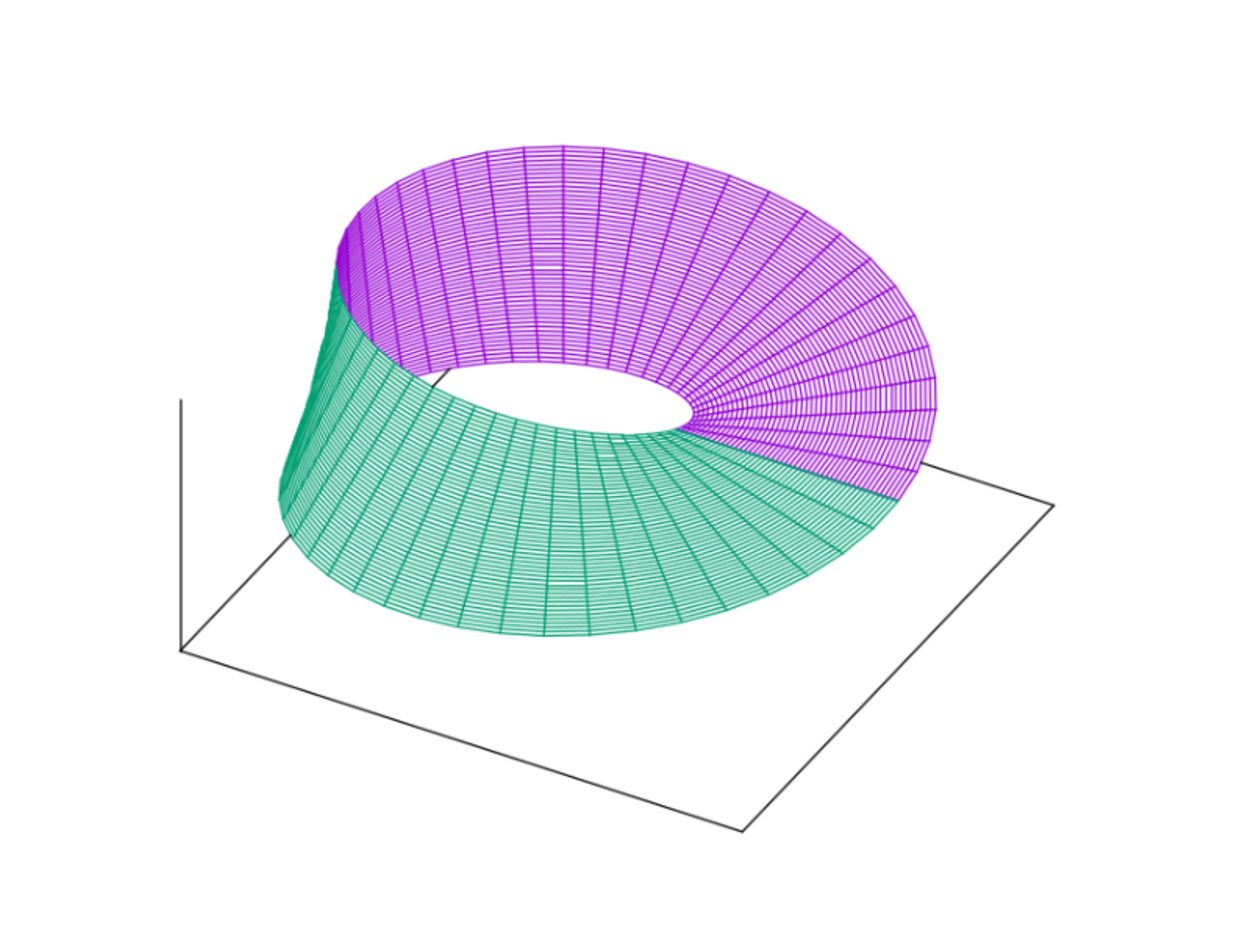
\includegraphics[scale=0.3]{eps/moebius}
		\caption{La banda de M\"obius es una superficie no orientable.}
		\label{fig:Moebius}
\end{figure}

\begin{definition}
	\index{Aplicación!de Gauss}
	Sea $S$ una superficie orientable. La función $N\colon S\to S^2$, $p\mapsto
	N(p)$, se conoce como la \textbf{aplicación de Gauss} de $S$. 
\end{definition}

Vimos que la normal a la esfera $S^2$ en el punto $p$ es
$N(p)=p$. Como la esfera puede definirse como $S^2=f^{-1}(0)$, donde
$f(x,y,z)=x^2+y^2+z^2-1$, entonces 
\begin{align*}
	T_{N(p)}S^2&=\ker (df)_{N(p)}\\
	&=\{v\in\R^3:\langle N(p),v\rangle=0\}
	=\{ v\in\R^3:\langle p,v\rangle=0\}=T_pS.
\end{align*}

\begin{lemma}
	\label{lem:N_u,N_v}
	Sea $X\colon U\to X(U)$ una parametrización de una superficie $S$ alrededor de $p\in S$ y sea $q=X^{-1}(p)$. 
	Entonces \[
		(N_X)_u(q)=(dN)_{p}(X_u(q)),\quad
		(N_X)_v(q)=(dN)_{p}(X_v(q)).
	\]
\end{lemma}

\begin{proof}
	Como $N_X=N\circ X\colon
	U\to S^2$, 
	\begin{align*}
		(N_X)_u(q)&=
		(dN_X)_{q}(1,0)
		=(d(N\circ X))_{q}(1,0)\\
		&=(dN)_{p}(dX)_{q}(1,0)
		=(dN)_p(X_u(q)).
	\end{align*}
	Análogamente se demuestra que $(N_X)_v(q)=(dN)_{p}(X_v(q))$. 
\end{proof}

Una transformación lineal $A\colon\R^n\to\R^n$ se dice \textbf{autoadjunta} si
$\langle Av,w\rangle=\langle v,Aw\rangle$ para todo $v,w\in\R^n$. 

\begin{theorem}
	Sean $S$ una superficie orientable y $p\in S$. Si $N$ es la aplicación de Gauss, entonces  
	$(dN)_p\colon T_pS\to T_{N(p)}S^2\simeq T_pS$ es audoadjunta. 
\end{theorem}

\begin{proof}
	Sea $X\colon U\to S$ una parametrización en $p$ y sea $q=X^{-1}(p)$. 
	Como $\{X_u(p),X_v(p)\}$ es una base de $T_pS$ basta ver que 
	\[
		\langle (dN)_p(X_u),X_v\rangle=\langle X_u,(dN)_p(X_v)\rangle
	\]
	en un entorno de $q$. 
	Sabemos que $\langle N_X,X_u\rangle=0$ alrededor de $q$. Al derivar esta expresión con
	respecto a la variable $v$ obtenemos 
	\[
		\langle (N_X)_v,X_u\rangle+\langle
	N_X,X_{uv}\rangle=0.
	\]
	Similarmente, al derivar $\langle N_X,X_v\rangle=0$ con
	respecto a la variable $u$ tenemos 
	\[
		\langle (N_X)_u,X_v\rangle+\langle
	N_X,X_{vu}\rangle=0. 
	\]
	Como $X_{uv}=X_{vu}$, 
	se concluye al usar el lema anterior que 
	\begin{align*}
		\langle (dN)_p(X_u),X_v\rangle
		&=\langle (N_X)_u,X_v\rangle\\
		&=\langle (N_X)_v,X_u\rangle
		=\langle (dN)_p(X_v),X_u\rangle.\qedhere
	\end{align*}
\end{proof}

\index{Curvaturas principales}
\index{Curvatura!gaussiana}
\index{Curvatura!media}
Las transformaciones lineales autoadjuntas tienen autovalores reales y pueden
diagonalizarse. En cada punto $p$ de nuestra superficie orientable $S$, el
endomorfismo $-(dN)_p\colon T_pS\to T_pS$ tiene dos autovalores reales
$k_1(p)\leq k_2(p)$. Estos valores son las \textbf{curvaturas principales} de
$S$ en $p$.  Se define la \textbf{curvatura gaussiana} de $S$ en $p$ como el
número 
\[
K(p)=\det(-(dN)_p)=k_1(p)k_2(p).
\]
La \textbf{curvatura media} de $S$ en $p$ es el número 
\[
	H(p)=-\frac12\trace(dN)_p=\frac12(k_1(p)+k_2(p)).
\]
Vale entonces que 
\[
	k_i(p)^2-2H(p)k_i(p)+K(p)=0
\]
para todo $i\in\{1,2\}$. Como la ecuación cuadrática $X^2-2HX+K=0$ tiene dos
soluciones reales, se deduce que $K(p)\leq H(p)^2$ para todo $p\in S$.

\begin{example}
	\index{Plano}
	Sea $S$ un plano. Como $N\colon S\to S^2$ es una constante, $(dN)_p=0$ para
	todo $p\in S$. Luego 
	$k_1(p)=k_2(p)=H(p)=K(p)=0$ en todo punto $p\in S$.
\end{example}

\begin{example}
	\index{Esfera}
	Sea $S$ la \textbf{esfera} de radio $r$ con centro en el origen y sea $p\in S$. Vimos que 
	$N(p)=p/r$. Calculemos la diferencial $(dN)_p$ en un vector tangente $v\in
	T_pS$. Sea $\alpha$ una curva en $S$ tal que $\alpha(0)=p$ y
	$\alpha'(0)=v$. Como $N\circ\alpha(t)=\frac1r\alpha(t)$, por definición de diferencial, 
	\[
		(dN)_p(v)=\frac{d}{dt}(N\circ\alpha)(0)=\frac1r\alpha'(0)=\frac1rv.
	\]
	Luego $-(dN)_p(v)=-\frac{1}{r}v$ para todo $v\in T_pS$ y, en particular, 
	\[
		k_1(p)=k_2(p)=-1/r,\quad
		H(p)=-\frac{1}{r},\quad
		K(p)=\frac{1}{r^2}.
	\]
\end{example}

%\begin{exercise}
%	Sea $S$ la superficie dada por $z=x^2-y^2$. Para $p=(0,0,0)$ calcule
%	$k_1(p)$, $k_2(p)$, $K(p)$ y $H(p)$.
%\end{exercise}

%\begin{exercise}
%	Sea $S$ la superficie dada por $X(u,v)=(u,v,u^3-3v^2u)$. Para $p=(0,0,0)$ calcule
%	$k_1(p)$, $k_2(p)$, $K(p)$ y $H(p)$.
%\end{exercise}

\begin{example}
	\label{exa:cilindro_recto:K}
	\index{Cilindro}
	Sea $r>0$ y sea $S=\{(x,y,z)\in\R^3:x^2+y^2=r^2\}$ el \textbf{cilindro recto} de
	radio $r$. Si $p=(x,y,z)\in S$, entonces $N(x,y,z)=\frac1r(x,y,0)$. Vamos
	a calcular $-(dN)_p(v)$, donde $v=(v_1,v_2,v_3)\in T_pS$. Sea $\alpha$ una
	curva en $S$ tal que $\alpha(0)=p$ y $\alpha'(0)=v$. Por definición,  
	\[
		-(dN)_p(v)=-\frac{d}{dt}(N\circ\alpha)(0)=-\frac1r(v_1,v_2,0).
	\]
	Tenemos que encontrar los autovalores de $-(dN)_p$. A simple vista vemos que 
	\[
		-(dN)_p(0,0,v_3)=(0,0,0)=0(0,0,v_3),\quad
		-(dN)_p(0,v_2,0)=-\frac1r(0,v_2,0).
	\]
	Como $k_1(p)=-1/r$ y $k_2(p)=0$ son los autovalores de $-(dN)_p$, se
	concluye que $K(p)=0$ y $H(p)=-\frac{1}{2r}$.
\end{example}

\begin{example}
	\label{exa:paraboloide_hiperbolico}
	\index{Paraboloide hyperbólico}
	Sea $S$ el \textbf{paraboloide hiperbólico} dado por $z=y^2-x^2$ que vemos en la
	figura~\ref{fig:hiperboloide}.  Calculemos las curvaturas de $S$ en el
	punto $p=(0,0,0)$. Sea $X\colon\R^2\to S$, 
	$X(u,v)=(u,v,v^2-u^2)$ y sea $q=X^{-1}(p)=(0,0)$.  Un cálculo directo
	muestra que $X_u(u,v)=(1,0,-2u)$, $X_v(u,v)=(0,1,2v)$, y 
	\begin{align*}
		&N_X(u,v)=\frac{1}{\sqrt{4u^2+4v^2+1}}(2u,-2v,1).
	\end{align*}
	Si $N$ es la aplicación de Gauss, entonces
	\begin{align*}
		&(dN)_p(X_u(q))=(dN)_p(1,0,0)=(N_X)_u(q)=(2,0,0),\\
	\shortintertext{y similarmente}
		&(dN)_p(X_v(q))=(dN)_p(0,1,0)=(N_X)_v(q)=(0,-2,0).
	\end{align*}
	Esto nos dice que $k_1(p)=-2$,
	$k_2(p)=2$, $K(p)=-4$ y $H(p)=0$. 
	\begin{figure}[h]
		\centering
    	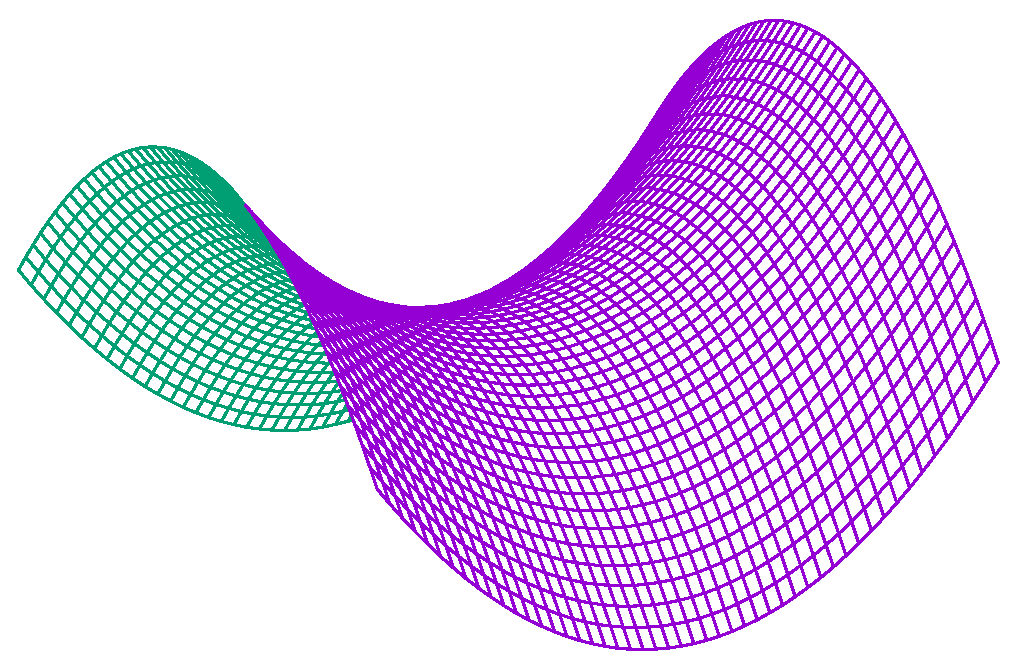
\includegraphics[scale=0.3]{eps/hyperbolic}
		\caption{El paraboloide hiperbólico.}
		\label{fig:hiperboloide}
	\end{figure}
\end{example}

\chapter{La primera forma fundamental} 

El producto interno de $\R^3$ induce un producto interno en el tangente $T_pS$
a $S$ en el punto $p$. De alguna forma, esto indica que $S$ hereda el producto
escalar natural que se tiene en el espacio ambiente, y gracias a esto podemos
medir longitud de curvas, ángulos y áreas en $S$ sin apelar a $\R^3$. 

\begin{definition}
	\index{Primera forma fundamental}
	La \textbf{primera forma fundamental} de una superficie $S$ en un punto $p$ 
	se define como la función
	\[
		\I_p\colon T_pS\to\R,\quad
		\I_p(v)=\langle v,v\rangle.
	\]
\end{definition}

\index{Coeficientes!de la primera forma fundamental}
Sea $X\colon U\to X(U)\subseteq S$ una parametrización local de una superficie
$S$ alrededor de un punto $p\in S$.  Los \textbf{coeficientes de la primera forma
fundamental} son 
\[
	E=\langle X_u,X_u\rangle,\quad
	F=\langle X_u,X_v\rangle,\quad
	G=\langle X_v,X_v\rangle.
\]
Por definición, $E$, $F$ y $G$ son funciones diferenciables. 

Calculemos algunas primeras formas fundamentales:

\begin{example}
	\index{Plano}
	El \textbf{plano} $z=0$ puede parametrizarse con 
	\[
	X(u,v)=(u,v,0).
	\]
	Como $X_u=(1,0,0)$ y $X_v=(0,1,0)$, los coeficientes de la primera forma
	fundamental son entonces $E=G=1$ y $F=0$. 
\end{example}

%	Calculemos ahora los coeficientes de la primera forma fundamental si
%	parametrizamos $z=0$ utilizando coordenadas polares, es decir con la
%	parametrización
%	\[
%		\overline{X}(r,\theta)=(r\cos\theta,r\sin\theta,0),
%	\]
%	Como $\overline{X}_r=(\cos\theta,\sin\theta,0)$ y
%	$\overline{X}_\theta=(-r\sin\theta,r\cos\theta,0)$, se concluye
%	$\overline{E}=1$, $\overline{F}=0$, $\overline{G}=r^2$.

\begin{example}
	\index{Cilindro}
	Consideremos la parametrización del \textbf{cilindro} 
	\[
	X(u,v)=(\cos v ,\sin v,u). 
	\]
	Como $X_u=(0,0,1)$ y $X_v=(-a\sin v ,a\cos v ,0)$, se conluye que $E=1$,
	$F=0$, $G=1$. 
\end{example}

Es interesante observar que las primeras formas fundamentales que calculamos
para el plano y el cilindro coinciden.

\begin{example}
	\index{Esfera}
	Consideremos la parametrización de la \textbf{esfera} dada por 
	\[
	X(u,v)=(\sin u\sin v,\cos u\sin v,\cos v).
	\]
	Como $X_u=(\cos u\sin v,-\sin u\sin v,0)$ y $X_v=(\sin u\cos v,-\cos
	u\cos v,-\sin v)$, se conluye que $E=\sin^2v$, $F=0$, $G=1$. 
\end{example}

\begin{example}
	\index{Cono}
	Consideremos la parametrización del \textbf{cono} dada por
	\[
		X(u,v)=(u\cos v,u\sin v,u).
	\]
	Como $X_u=(\cos v,\sin v,1)$ y $X_v=(-u\sin v,u\cos v,0)$, se concluye inmediatamente que
	$E=2$, $F=0$, $G=u^2$.
\end{example}

\begin{example}
	\index{Helicoide}
	Consideremos la parametrización del \textbf{helicoide} 
	\[
		X(u,v)=(v\cos u,v\sin u,u),
	\]
	donde $0<u<2\pi$ y $v\in\R$. Un cálculo sencillo muestra que $E=1+v^2$, $F=0$ y $G=1$. 
\end{example}

\index{Primera forma fundamental!longitud de curvas}
La primera forma fundamental da la geometría de la superficie. Podemos por
ejemplo utilizarla para calcular la \textbf{longitud de curvas} en $S$. Sea
$\alpha\colon I\subseteq\R\to S\subseteq\R^3$ una curva en $S$. Entonces
\[
	L(\alpha)=\int_I\sqrt{I_p(\alpha'(t))}dt.
\]

\index{Primera forma fundamental!ángulo entre curvas}
Podemos utilizar la primera forma fundamental para calcular \textbf{ángulos entre
curvas}: si $\alpha$ y $\beta$ son curvas en una superficie $S$ tales que
$\alpha(0)=\beta(0)$, y $\theta$ es el ángulo que forman $\alpha'(0)$ y
$\beta'(0)$, entonces 
\[
	\cos\theta=\frac{\langle \alpha'(0),\beta'(0)\rangle}{\|\alpha'(0)\|\|\beta'(0)\|}=\frac{F}{\sqrt{EG}}.
\]

\index{Dominio}
\index{Primera forma fundamental!área}
También podemos utilizar la primera forma fundamental para el \textbf{cálculo de áreas}.
Recordemos que un \textbf{dominio} en una superficie $S$ es un abierto conexo
$D\subseteq S$ tal que $\partial D$ es la imagen del círculo $S^1$ por un
homeomorfismo diferenciable a trozos. Una \textbf{región} $R$ es la unión de un
dominio $D$ junto con su frontera $\partial D$. Definimos entonces
el área de un dominio $R$ como
\[
	\text{área}(R)=\int_{X^{-1}(R)}\|X_u\times X_v\|dudv.
\]
Esta definición no depende de la parametrización $X$ pues si $Y\colon V\to
Y(V)$ es otra parametrización tal que $R\subseteq X(U)\cap Y(V)$, la fórmula de
cambio de variables implica que
\[
	\int_{X^{-1}(U)}\|X_u\times X_v\|dudv=\int_{Y^{-1}(R)}\|Y_u\times Y_v\|dudv.
\]

\index{Identidad de Lagrange}
Para ver que podemos escribir el área en términos de la primera forma fundamental necesitamos 
la \textbf{identidad de Lagrange}:
\[
	\langle v,v\rangle\langle w,w\rangle-\langle v,w\rangle^2=\langle v\times w,v\times w\rangle.
\]
para todo $v,w\in\R^3$. Para demostrar rápidamente esta identidad alcanza con recordar que si $\theta$ es el ángulo que forman $v$ y $w$, entonces 
\begin{align*}
\langle v,w\rangle^2=\langle v,v\rangle\langle w,w\rangle\cos^2\theta,
&&\langle v\times w,v\times w\rangle^2=\langle v,v\rangle\langle w,w\rangle\sin^2\theta. 
\end{align*}
Luego
\begin{align*}
	\langle v,v\rangle\langle w,w\rangle-\langle v\times w,v\times w\rangle^2
	&=\langle v,v\rangle\langle w,w\rangle(1-\sin^2\theta)
	=\langle v,w\rangle^2.
\end{align*}

Se tiene entonces la siguiente fórmula:
\[
	\text{área}(R)=\int_{X^{-1}(U)}\sqrt{EG-F^2}dudv.
\]

\chapter{La segunda forma fundamental} 

\index{Segunda forma fundamental}
La \textbf{segunda forma fundamental} de una superficie orientable $S$ en un
punto $p$ se define como la función
\[
	\II_p\colon T_pS\times T_pS\to\R,\quad
	(v,w)\mapsto -\langle (dN)_p(v),w\rangle.
\]

Veamos una interpretación geométrica. Sea $\gamma$ una curva en $S$
parametrizada por longitud de arco. Como el vector normal $N$ a la superficie
$S$ es unitario y perpendicular a $\gamma'$, los vectores $N$ y
$N\times\gamma'$ son perpendiculares y unitarios. Además
$1=\|\gamma'|^2=\langle\gamma',\gamma'\rangle$ pues $\gamma$ está parametrizada
por longitud de arco, al derivar obtenemos que
$0=\langle\gamma'',\gamma'\rangle$. Como $\gamma''$ es perpendicular a
$\gamma'$, existen funciones $\kappa_N$ y $\kappa_g$ tales que
\begin{equation}
	\label{eq:Nyg}
	\gamma''=\kappa_NN+\kappa_gN\times\gamma'
\end{equation}

\index{Curvatura!normal}
\index{Curvatura!geodésica}
La función $\kappa_N$ se conoce como la \textbf{curvatura normal} de $\gamma$.
La función  $\kappa_g$ es la \textbf{curvatura geodésica} de $\gamma$.  Como
$\{\gamma',N,N\times\gamma'\}$ es un conjunto ortonormal, la
fórmula~\eqref{eq:Nyg} implica que
\[
	\kappa_N=\langle\gamma'',N\rangle,\quad
	\kappa_g=\langle\gamma'',N\times\gamma'\rangle.
\]

\begin{lemma}
	Sea $\kappa$ la curvatura de $\gamma$ vista como curva en $\R^3$. Si $n$ es el
	vector normal a la curva $\gamma$, sea $\theta$ tal que 
	$\cos\theta=\langle n,N\rangle$. 
	Valen las siguientes fórmulas:
	\begin{align}
		&\kappa^2=\kappa_N^2+\kappa_g^2,&&
		\kappa_N=\kappa\cos\theta, &&
		\kappa_g=\pm\kappa\sin\theta.
	\end{align}
\end{lemma}

\begin{proof}
	Como $\gamma$ está parametrizada por longitud de arco y los vectores $N$ y
	$N\times\gamma'$ son unitarios, la curvatura $\kappa$ de $\gamma$ verifica que 
	\[
		\kappa^2=\|\gamma''\|^2
		=\langle\gamma'',\gamma''\rangle
		=\langle\kappa_NN+\kappa_gN\times\gamma',\kappa_NN+\kappa_gN\times\gamma'\rangle
		=\kappa_N^2+\kappa_g^2.
	\]

	Como $\gamma''=\kappa n$, entonces
	$\kappa\cos\theta=\langle\kappa n,N\rangle=\langle \gamma'',N\rangle=\kappa_N$. 

	De la fórmula 
	$\kappa^2=\kappa_N^2+\kappa_g^2=\kappa^2\cos^2\theta+\kappa_g^2$ se obtiene inmediatamente 
	que $\kappa_g^2=\kappa^2(1-\cos^2\theta)$ y luego 
	$\kappa_g=\pm\kappa\sin\theta$.
\end{proof}

Demostraremos a continuación que dos curvas de una superficie que se cortan en
un mismo punto $p$ y tienen tangentes paralelos en $p$ tienen la misma
curvatura normal en ese punto $p$.

\begin{theorem}[Meusnier]
	\index{Teorema!de Meusnier}
	Sea $S$ una superficie orientable y sea $\gamma$ una curva en $S$
	parametrizada por longitud de arco.  Entonces
	\[
		\kappa_N(s)=\II_{\gamma(s)}(\gamma'(s)).
	\]
\end{theorem}

\begin{proof}
	Si $N(s)=N(\gamma(s))$, entonces
	$N'(s)=(dN)_{\gamma(s)}(\gamma'(s))$. Además 
	como $\langle
	N(s),\gamma'(s)\rangle=0$, al derivar obtenemos que $\langle
	N'(s),\gamma'(s)\rangle+\langle N(s),\gamma''(s)\rangle=0$. 
	Esto implica que 
	\begin{align*}
		\II_{\gamma(s)}(\gamma'(s))
		&=\langle -(dN)_{\gamma(s)}(\gamma'(s)),\gamma'(s)\rangle\\
		&=\langle -N'(s),\gamma'(s)\rangle
		=\langle N(s),\gamma''(s)\rangle
		%=\langle N(s),\kappa(s)n(s)\rangle=\kappa(s)\cos\theta(s)
		=\kappa_N(s).\qedhere
	\end{align*}
\end{proof}

\index{Fórmula!de Euler}
Veamos cómo calcular la curvatura normal en un punto $p$ a lo largo de una
dirección $v$ de $T_pS$. Supongamos que $\|v\|=1$ y sea $\{e_1,e_2\}$ una base
ortonormal de $T_pS$ tal que $-(dN)_p(e_i)=k_ie_i$ para $i\in\{1,2\}$. Podemos
escribir entonces
\[
	v=\cos\theta e_1+\sin\theta e_2,
\]
pues $\cos\theta=\langle v,e_1\rangle$ y
$\sin\theta=\cos(\frac{\pi}{2}-\theta)=\langle v,e_2\rangle$. Luego
\begin{equation}
	\label{eq:Euler}
\begin{aligned}
	\kappa_N&=\II_p(v)=-\langle (dN)_p(v),v\rangle\\
	&=-\langle (dN)_p(\cos\theta e_1+\sin\theta e_2),\cos\theta e_1+\sin\theta e_2\rangle\\
	&=k_1\cos^2\theta +k_2\sin^2\theta.
\end{aligned}
\end{equation}
La expresión~\eqref{eq:Euler} se conoce como la \textbf{fórmula de Euler}. 

\begin{theorem}
	\label{thm:k1min_k2max}
	Si $S$ es una superficie orientada y $p\in S$, entonces
	\[
		k_1(p)=\min\{\II_p(v):v\in T_pS\},\quad
		k_2(p)=\max\{\II_p(v):v\in T_pS\}.
	\]
\end{theorem}

\begin{proof}
	Veamos que 
	como
	$k_1(p)\leq k_2(p)$, entonces $k_1(p)$ es el mínimo
	y $k_2(p)$) 
	es el máximo de las curvaturas normales de las curvas de la superficie que
	pasan por el punto $p$. En efecto, 
	\begin{align*}
		\kappa_N&=(\cos^2\theta)k_1+(\sin^2\theta)k_2\\
		&=k_1(1-\sin^2\theta)+k_2\sin^2\theta=(k_2-k_1)\sin^2\theta+k_1\geq k_1;
	\end{align*}
	y vale la igualdad si y sólo si $\theta\in\{0,\pi\}$ (es decir, si y sólo si
	$\gamma'$ es paralelo a $e_1$). Similarmente vemos que $\kappa_N\leq k_2$ y vale la
	igualdad si y sólo si $\gamma'$ y $e_2$ son paralelos.
\end{proof}


%Sabemos que para cada superficie orientable $S$, $(dN)_p$ es diagonalizable.
%Existe entonces una base ortonormal $\{e_1,e_2\}$ de $T_pS$ y existen funciones
%$k_1$ y $k_2$ tales que $k_1\leq k_2$ y $(dN)_p(e_i)=-k_ie_i$ para
%$i\in\{1,2\}$.  Las funciones $k_1$ y $k_2$ se conocen como las
%\textbf{curvaturas principales} de la superficie y los autovectores $e_1$ y
%$e_2$ se conocen como las \textbf{direcciones principales}.

\begin{definition}
	\index{Punto!elíptico}
	Un punto $p$ de una superficie se dice \textbf{elíptico} si $K(p)>0$. 
\end{definition}

Vimos que todo punto de la esfera es elíptico. 

\begin{theorem}
	\label{thm:compacta_eliptico}
	Toda superficie compacta contiene al menos un punto elíptico. 
\end{theorem}

\begin{proof}
	Sea $h\colon S\to\R$, $h(x)=\|x\|^2$. Como $h$ es continua y $S$ es
	compacto, $h$ alcanza su máximo en un punto $p\in S$. Sea $\gamma$ una
	curva en $S$ parametrizada por longitud de arco tal que $\gamma(0)=p$. Como
	entonces
	$h\circ\gamma$ alcanza su máximo en $t=0$, 
	\[
		\frac{d}{dt}(h\circ\gamma)(0)=0,\quad
		\frac{d^2}{dt^2}(h\circ\gamma)(0)\leq 0.
	\]
	Como
	$\gamma$ está parametrizada por longitud de arco, 
	al derivar $h\circ\gamma(t)=\langle \gamma(t),\gamma(t)\rangle$ obtenemos 
	\begin{align*}
		&\frac{d}{dt}(h\circ\gamma)(t)=2\langle \gamma'(t),\gamma(t)\rangle,\\
		&\frac{d^2}{dt^2}(h\circ\gamma)(t)=2\langle \gamma''(t),\gamma(t)\rangle+2\langle \gamma'(t),\gamma'(t)\rangle=2(1+\langle\gamma''(t),\gamma(t)\rangle.
	\end{align*}
	Al evaluar la primera fórmula en $t=0$,
	$\langle p,\gamma'(0)\rangle=0$, que nos dice $p$ es ortogonal a cualquier vector tangente a
	$S$ en $p$. Luego $N(p)=\pm p/\|p\|$. Al evaluar la segunda fórmula en $t=0$,
	\[
		\langle \gamma''(0),p\rangle+1\leq 0.
	\]
	Sin perder generalidad supongamos que $N(p)=p/\|p\|$. Como por definición 
	curvatura normal de $\gamma$ en $t=0$ es 
	$\kappa_N(0)=\langle\gamma''(0),N(p)\rangle$, 
	la desigualdad anterior puede reescribirse
	entonces como $\kappa_N(p)\leq -1/\|p\|$ y esta desigualdad vale para cualquier curvatura normal. 
	Como $k_1(p)$ y $k_2(p)$ son el
	mínimo y el máximo de las curvaturas normales, se concluye que 
	$k_j(p)\leq-1/\|p\|$ para todo $j\in\{1,2\}$. En consecuencia, 
	\[
		K(p)=k_1(p)k_2(p)\geq\frac{1}{\|p\|^2}>0.
	\]
	De forma similar se trata el caso en que $N(p)=-p/\|p\|$.
\end{proof}

\index{Superficie!mínima}
Las superficies donde la curvatura media es siempre nula son de interés 
y se conocen como \textbf{superficies mínimas}. 

\begin{corollary}
	No existen superficies mínimas compactas.
\end{corollary}

\begin{proof}
	Si $S$ es una superficie mínima, entonces, como $H(p)=0$ para todo $p\in
	S$, se tiene que $-k_1(p)=k_2(p)$. Como entonces $K(p)=k_1(p)k_2(p)\leq 0$, 
	el teorema anterior implica que $S$ no puede ser compacta.
\end{proof}

En el teorema~\ref{thm:compacta_eliptico} es necesario suponer que la
superficie es compacta.  Veremos por ejemplo que la superficie
$z=\frac12(y^2-x^2)$ tiene curvatura gaussiana siempre negativa (en este caso,
nuestra superficie no es acotada).  Puede probarse además que
$S=\{(x,y,z)\in\R^3:x^2+y^2<1,\,z=0\}$ es una superficie que tiene curvatura
siempre cero (en este caso, nuestra superficie no es cerrada). Observemos que
no tiene sentido considerar $\{x^2+y^2\leq 1,\,z=0\}$ ya que este conjunto no
es una superficie.

\begin{definition}
	\index{Punto!hiperbólico}
	Un punto $p$ de una superficie se dice \textbf{hiperbólico} si $K(p)<0$. 
\end{definition}

Vimos en el ejemplo~\ref{exa:paraboloide_hiperbolico} que el punto $(0,0,0)$ es
un punto hiperbólico del paraboloide hiperbólico $z=y^2-x^2$. 

\begin{definition}
	\index{Punto!parabólico}
	Un punto $p$ de una superficie se dice \textbf{parabólico} si $K(p)=0$ y
	además $(dN)_p\ne 0$. 
\end{definition}

Vimos en el ejemplo~\ref{exa:cilindro_recto:K} que los puntos del cilindro son
parabólicos.

\begin{definition}
	\index{Punto!plano}
	Diremos que un punto $p$ de una superficie es \textbf{plano} si 
	$(dN)_p=0$. 
\end{definition}

Obviamente todo punto de un plano es un punto plano. Más adelante veremos
ejemplos no triviales de puntos planos. 
%Veamos un ejemplo no
%trivial de puntos planos de superficies:
%
%\begin{example}
%	
%\end{example}

\begin{definition}
	\index{Punto!umbílico}
	Un punto $p$ de una superficie se dice \textbf{umbílico} si $k_1(p)=k_2(p)$. 
\end{definition}

Vimos que todo punto de la esfera o de un plano es umbílico. Veremos más
adelante que el punto $(0,0,0)$ es un punto umbílico y no plano de la
superficie $z=x^2+y^2$.

\medskip
\index{Segunda forma fundamental!coeficientes}
\index{Coeficientes!de la segunda forma fundamental}
Nuestro objetivo ahora es entender qué significan estas definiciones 
y poder realizar cálculos. 
Vamos encontrar los \textbf{coeficientes de la segunda forma fundamental}. 
Sea $X\colon U\to X(U)$ una parametrización de una superficie $S$ y  
sea $\alpha$ una curva en $S$, digamos
\[
	\alpha(t)=X(u(t),v(t)).
\]
Al derivar obtenemos
%$\alpha'(t)=X_u(u(t),v(t))u'(t)+X_v(u(t),v(t))v'(t)$. 
%Abreviadamente escribiremos esta fórmula como 
\[
	\alpha'(t)=X_uu'(t)+X_vv'(t),
\]
donde sabemos que $X_u$ denota a la función $X_u(u(t),v(t))$ y $X_v$ denota a
la función $X_v(u(t),v(t))$. Queremos calcular
\begin{align*}
	\II_{\alpha(t)}(\alpha'(t))&=\langle -(dN)_{\alpha(t)}(\alpha'(t)),\alpha'(t)\rangle.
\end{align*}
Al desarrollar la expresión 
\begin{align*}
	\II_{\alpha(t)}(\alpha'(t))=\langle -(dN)_{\alpha(t)}(X_uu'(t)+X_vv'(t)),X_uu'(t)+X_vv'(t))\rangle
\end{align*}
obtenemos
\begin{multline*}
	\II_{\alpha(t)}(\alpha'(t))=u'(t)^2\langle -(dN)_p(X_u),X_u\rangle
	+u'(t)v'(t)\langle -(dN)_p(X_u),X_v\rangle\\
	+u'(t)v'(t)\langle -(dN)_p(X_v),X_u\rangle
	+v'(t)^2\langle -(dN)_p(X_v),X_v\rangle.
\end{multline*}
Como además $(dN)_{\alpha(t)}(X_u)=(N_X)_{u}$ y $(dN)_{\alpha(t)}(X_v)=(N_X)_v$, $X_{uv}=X_{vu}$ y 
\begin{align*}
	&\langle -(dN)_{\alpha(t)}X_u,X_u\rangle=\langle -(N_X)_u,X_u\rangle=\langle N_X,X_{uu}\rangle,\\
	&\langle -(dN)_{\alpha(t)}X_u,X_v\rangle=\langle -(N_X)_u,X_v\rangle=\langle N_X,X_{uv}\rangle,\\
	&\langle -(dN)_{\alpha(t)}X_v,X_u\rangle=\langle -(N_X)_v,X_u\rangle=\langle N_X,X_{vu}\rangle,\\
	&\langle -(dN)_{\alpha(t)}X_v,X_v\rangle=\langle -(N_X)_v,X_v\rangle=\langle N_X,X_{vv}\rangle.
\end{align*}
se concluye que 
\[
	\II_{\alpha(t)}(\alpha'(t))=u'(t)^2e+2u'(t)v'(t)f+v'(t)^2g,
\]
donde
\begin{align*}
	e=\langle N_X, X_{uu}\rangle, && 
	f=\langle N_X, X_{uv}\rangle, &&
	g=\langle N_X, X_{vv}\rangle.
\end{align*}
Es importante recordar que $e$, $f$ y $g$ son en realidad funciones $U\to\R$. 

\begin{proposition}
	Sea $X\colon U\to X(U)$ una parametrización de una superficie $S$. Las
	funciones $e,f,g\colon U\to\R$ son diferenciables. 
\end{proposition}

\begin{proof}
	Las funciones $e,f,g\colon U\to\R$ son diferenciables pues pueden
	escribirse como
	\begin{align*}
		&e=\langle N_X, X_{uu}\rangle=\frac{1}{\|X_u\times X_v\|}\langle X_u\times X_v,X_{uu}\rangle,\\
		&f=\langle N_X, X_{uv}\rangle=\frac{1}{\|X_u\times X_v\|}\langle X_u\times X_v,X_{uv}\rangle,\\
		&g=\langle N_X, X_{vv}\rangle=\frac{1}{\|X_u\times X_v\|}\langle X_u\times X_v,X_{vv}\rangle.\qedhere
	\end{align*}
\end{proof}

Estamos ahora en condiciones de explicar la terminología introducida. Sea $S$
una superficie y $p\in S$. Sabemos que en un entorno de $p$, $S$ es la
superficie dada por el gráfico de una función $h$ diferenciable. Sea entonces $X$
una parametrización en $p$ de la forma
\[
	X(u,v)=(u,v,h(u,v)),
\]
donde $h$ es una función diferenciable. 

Para simplificar la presentación supongamos que $p=(0,0,0)$ y que $T_pS$ es el
plano $z=0$ con normal $N_X=(0,0,1)$. Como $p=(0,0,0)=X(0,0)$, entonces
$h(0,0)=0$. Además 
\[
	X_u=(1,0,h_u),\quad
	X_v=(0,1,h_v),
\]
y entonces 
$h_u(0,0)=h_v(0,0)=0$ pues $X_u\times X_v$ es perpendicular al
plano $T_pS$.  El teorema de Taylor nos permite escribir
\begin{align*}
	h(u,v)=h(0,0)&+uh_u(0,0)+vh_v(0,0)\\
	&+\frac12(u^2h_{uu}(0,0)+2uvh_{uv}(0,0)+v^2h_{vv}(0,0))+\cdots
\end{align*}
donde los puntos suspensivos indican términos que involucran monomios en $u$ y
$v$ de orden $\geq3$. Esto nos dice que cerca del $(0,0)$ la función $h$ se
parece a la función 
\[
	z(u,v)=\frac12(u^2h_{uu}(0,0)+2uvh_{uv}(0,0)+v^2h_{vv}(0,0))
\]
y luego $X(u,v)$ es aproximadamente igual a $(u,v,z(u,v))$ cerca de $(0,0)$. 
Como
\[
	X_{uu}=(0,0,h_{uu}),\quad
	X_{uv}=(0,0,h_{uv}),\quad
	X_{vv}=(0,0,h_{vv}),
\]
se tiene que 
\begin{align*}
	h(u,v)
	&=\langle X(u,v),N\rangle
	\sim z(u,v)\\
	&=\frac12(u^2h_{uu}(0,0)+2uvh_{uv}(0,0)+v^2h_{vv}(0,0))\\
	&=\frac12(u^2\langle X_{uu}(0,0),N\rangle +2uv\langle X_{uv}(0,0),N\rangle +v^2\langle X_{vv}(0,0),N\rangle)\\
	&=\frac12(u^2e(0,0)+2uvf(0,0)+v^2g(0,0))\\
	&=\frac12\II_p(u,v,0).
\end{align*}

Sean $e_1$ y $e_2$ las direcciones principales de $S$ en $p$ y para simplificar
la presentación supongamos que $e_1=(1,0,0)$ y $e_2=(0,1,0)$.  Sean $k_1$ y
$k_2$ tales que $-(dN)_p(e_i)=k_ie_i$ para $i\in\{1,2\}$. Si escribimos al
vector tangente $(x,y,0)$ como 
\[
	(x,y,0)=xe_1+ye_2,
\]
entonces 
\[
	-(dN)_p(x,y,0)=-(dN)_p(xe_1+ye_2)=xk_1e_1+yk_2e_2=(xk_1,xk_2,0)
\]
y en consecuencia
\begin{align*}
	2z(x,y)&=\II_p(x,y,0)\\
	&=\langle -(dN)_p(x,y,0),(x,y,0)\rangle
	=\langle (k_1x,k_2y,0),(x,y,0)\rangle
	=k_1x^2+k_2y^2.
\end{align*}
Esto nos dice que cerca del punto $p$ la superficie $S$ se parece a la superficie dada
por la ecuación 
\begin{equation}
	\label{eq:z=f(x,y)}
	2z=k_1x^2+k_2y^2. 
\end{equation}
Hay entonces cuatro casos para considerar: 
\begin{itemize}
	\item Si $k_1k_2>0$, entonces~\eqref{eq:z=f(x,y)} es la ecuación de un
	paraboloide elíptico y por eso $p$ es un punto elíptico.  \item Si
		$k_1k_2<0$, entonces~\eqref{eq:z=f(x,y)} es la ecuación de un
		paraboloide hiperbólico y por eso $p$ es un punto hiperbólico.
	\item Si $k_1k_2=0$ y $k_1+k_2\ne 0$, entonces~\eqref{eq:z=f(x,y)} es la
		ecuación de un cilindro parabólico y por eso $p$ es un punto
		parabólico.
	\item Si $k_1=k_2=0$, entonces~\eqref{eq:z=f(x,y)} es la ecuación de un
		plano y por eso $p$ es un punto plano.
\end{itemize}

\index{Curvatura!gaussiana, interpretación geométrica}
La explicación anterior motiva además otra interpretación geométrica de la
curvatura gaussiana. Si $p$ es un punto de una superficie $S$ entonces valen
las siguientes afirmaciones:
\begin{itemize}
	\item Si $K(p)>0$, existe un entorno $V$ de $p$ en $S$ tal que todo
		punto de $V$ está de un mismo lado del plano $p+T_pS$. 
			$S\cap U\setminus\{p\}$ son disjuntos. 
		\item Si $K(p)<0$, todo entorno $p$ contiene puntos de ambos lados de $p+T_pS$. 
			entre el plano $p+T_pS$ y el conjunto $S\cap U\setminus\{p\}$ es no vacía.
\end{itemize}

Como consecuencia de este resultado podríamos demostrar que toda superficie con
curvatura gaussiana positiva es orientable. 

%\begin{proof}
%	Sea $X$ una parametrización alrededor de $p$ tal que $X(0,0)=p$ y 
%	sea 
%	\[
%		h(u,v)=\langle N(p),X(u,v)-p\rangle.
%	\]	
%	El desarrollo de Taylor de $h$ alrededor de $(0,0)$ es
%	\begin{align*}
%		h(u,v)=h(0,0)h_u(0,0)u&+h_v(0,0)v\\
%		&+\frac12(h_{uu}(0,0)u^2+2h_{uv}(0,0)uv+h_{vv}(0,0)v^2)+R(u,v),
%	\end{align*}
%	donde $\lim_{(u,v)\to(0,0)}\frac{R(u,v)}{u^2+v^2}=0$. Por definición, 
%	\[
%		h(0,0)=h_u(0,0)=h_v(0,0)=0,\quad
%		h_{uu}(0,0)=e,\quad
%		h_{uv}(0,0)=f,\quad
%		h_{vv}(0,0)=g.
%	\]
%	y luego
%	\[
%		h(u,v)=\frac12(eu^2+2fuv+gv^2)+R(u,v).
%	\]
%	\framebox{completar}
%\end{proof}
%
%El teorema anterior nos dice que en caso en que la curvatura sea positiva en un
%cierto punto $p$, en un entorno de ese punto $p$ la superficie quedará
%completamente de un lado del plano tangente en $p$. Si en cambio la curvatura
%es negativa en $p$, entonces en un entorno de $p$ la superficie quedará a ambos
%lados del plano tangente en $p$.  Como consecuencia del teorema anterior se
%tiene que toda superficie con curvatura estrictamente positiva en todos sus
%puntos es orientable ya que puede tomarse $N$ como el vector que apunta siempre
%hacia afuera de la superficie.


% IMPORTANTE
% lo que asumí que pasa, en realidad pasa siempre. Se necesita usar el teorema de la función inversa para superficies
% y el corolario que dice que localmente S es el gráfico de una función diferenciable con dominio en el plano tangente. 
% Este truco lo hace MR en la demostración del teorema de Hilbert (ver teorema 3.47 y proposición 2.23) 

% puede demostrarse
%que un entorno de $p$ la superficie $S$ es el gráfico de una función
%diferenciable sobre cualquier plano que no contenga al normal $N(p)$. 

%\index{Superficie!conexa}
%Recordemos que una superficie $S$ se dice \textbf{conexa} si dados dos $p,q\in
%S$ existe una curva continua $\gamma\colon [0,1]\to S$ tal que $\gamma(0)=p$ y
%$\gamma(1)=q$. 

%\index{Función!localmente constante}
%Antes de caracterizar los puntos umbílicos necesitamos un lema sobre funciones localmente constantes con dominio conexo. 
%Una función $f\colon A\to B$ se dice \textbf{localmente constante} si para cada
%$a\in A$ existe un entorno $U$ de $a$ tal que $f(x)=b$ para todo $x\in U$.
%
%\begin{lemma}
%	Si $f\colon A\to B$ es localmente constante y
%	$A$ es conexo, entonces $f$ es
%	constante. 
%\end{lemma}
%
%\begin{proof}
%	Sea $a\in A$ y supongamos que $f(a)=b$. El conjunto \[
%		C=f^{-1}(b)=\{x\in A:f(x)=b\}
%	\]
%	es no vacío y cerrado. Veamos que $C$ es abierto: si
%	$x\in C$, existe un entorno $U\subseteq C$ de $x$ tal que $f|_U=b$. 
%	Luego $U\subseteq C$ y entonces $C$ es abierto.  Como $A$ es conexo y
%	$C$ es un conjunto no vacío, abierto y cerrado, se concluye que $C=A$.
%\end{proof}
%
%Recordemos que una superficie $S$ se dice \textbf{conexa} si dados dos $p,q\in
%S$ existe una curva continua $\gamma\colon [0,1]\to S$ tal que $\gamma(0)=p$ y
%$\gamma(1)=q$. 

\index{Superficie!totalmente umbílica}

\begin{theorem}
	\label{thm:umbilico}
	Si $S$ es una superficie conexa tal que todos sus puntos son umbílicos,
	entonces $S$ es un abierto de un plano o de una esfera.
\end{theorem}

\begin{proof}
	Sea $X\colon U\to X(U)\subseteq S$ una parametrización. Sin pérdida de
	generalidad podemos suponer que $U$ es conexo.  Por el
	lema~\ref{lem:N_u,N_v}, 
	\[
		(dN)_{X(u,v)}X_u(u,v)=(N_X)_u(u,v),\quad
		(dN)_{X(u,v)}X_v(u,v)=(N_X)_v(u,v)
	\]
	para todo $(u,v)\in U$. Como el punto $X(u,v)$ es umbílico, en ese punto
	las curvaturas principales coinciden y luego $(dN)_{X(u,v)}$ es un múltiplo
	escalar de la identidad del tangente a $S$ en $X(u,v)$. Esto implica que
	existe una función $\lambda\colon U\to\R$ tal que 
	\[
		(dN)_{X(u,v)}(w)=\lambda(u,v)w
	\]
	para todo $w\in T_{X(u,v)}S$. Como 
	\begin{equation}
		\label{eq:NcircX}
		(N_X)_u=\lambda X_u,\quad
		(N_X)_v=\lambda X_v.
	\end{equation}
	la función $\lambda$ resulta diferenciable. En efecto, las funciones
	$(N_X)_u$ y $X_u$ son diferenciables y vale que $\langle (N_X)_u,X_u\rangle=\langle \lambda X_u,X_u\rangle=\lambda\langle
	X_u,X_u\rangle$. Como $X_u\ne 0$, podemos escribir a $\lambda$ como 
	\[
		\lambda=\frac{\langle (N_X)_u,X_u\rangle}{\|X_u\|^2}.
	\]

	Al derivar las fórmulas~\eqref{eq:NcircX} obtenemos
	\[
		(N_X)_{uv}=\lambda_vX_u+\lambda X_{uv},\quad
		(N_X)_{vu}=\lambda_uX_v+\lambda X_{vu}
	\]
	y luego $\lambda_uX_v=\lambda_vX_u$. Pero como $X_u$ y $X_v$ son
	linealmente independientes, se concluye que $\lambda_u=\lambda_v=0$. Luego
	$\lambda$ es una función constante pues $U$ es conexo.

	Vamos ahora a distinguir dos casos. 
	
	Supongamos primero que $\lambda=0$. Las fórmulas de~\eqref{eq:NcircX}
	implican entonces que $N_X$ es constante. Como
	\begin{align*}
		&\frac{\partial}{\partial u}\langle X(u,v),N_X\rangle=\langle X_u(u,v),N_X\rangle=0,\\
		&\frac{\partial}{\partial v}\langle X(u,v),N_X\rangle=\langle X_v(u,v),N_X\rangle=0,
	\end{align*}
	existe una constante $c\in\R$ tal que $\langle X(u,v),N_X\rangle=c$ para todo
	$(u,v)\in U$. Luego $X(U)$ está contenido en el plano $\{v\in\R^3:\langle
	v,N_X\rangle=c\}$. 

	Supongamos ahora que $\lambda\ne0$. Por las fórmulas de~\eqref{eq:NcircX}
	sabemos que
	\[
		\frac{\partial}{\partial u}\left(X(u,v)-\frac{1}{\lambda}N_X(u,v)\right)=
		\frac{\partial}{\partial v}\left(X(u,v)-\frac{1}{\lambda}N_X(u,v)\right)=0,
	\]
	y luego existe un $c\in\R^3$ tal que $X(u,v)-\frac{1}{\lambda}N_X(u,v)=c$
	para todo $(u,v)\in U$.  Como entonces
	\[
		\|X(u,v)-c\|^2=\frac{1}{\lambda^2}\langle N_X,N_X\rangle=\frac{1}{\lambda^2},
	\]
	se concluye que $X(U)$ queda contenido en una esfera de radio
	$\frac{1}{|\lambda|}$.

	Quedó demostrado entonces el teorema en el caso en que la superficie pueda
	cubirse con una única parametrización. Probamos además que cada parche
	queda contenido en un plano o en una esfera. Si dos parches tienen
	intersección no vacía, entonces ambos estarán contenidos en la misma esfera
	o en el mismo plano. 
%	Sean ahora $p,q\in S$. Como $S$ es conexa, existe una curva continua
%	$\gamma\colon [0,1]\to S$ tal que $\gamma(0)=p$ y $\gamma(1)=q$. Para cada
%	$t\in[0,1]$ consideramos una parametrización $X_t\colon U_t\to S$ alrededor
%	del punto $\gamma(t)\in S$. Como $\gamma$ es continua y el intervalo
%	$[0,1]$ es compacto, $\gamma([0,1])$ es un conjunto compacto que puede
%	cubrirse con los abiertos $U_t$. Existen entonces finitos
%	$t_1,\dots,t_k\in[0,1]$ tales que
%	\[
%		\gamma([0,1])\subseteq \bigcup_{i=1}^k U_i.
%	\]
%	Como cada $X(U_j)$ es parte de un plano o parte de una esfera, todos los
%	$X(U_j)$ tienen que ser parte de ese mismo plano o de esa misma esfera.
\end{proof}

Para obtener un corolario del teorema anterior
necesitamos un lema:

\begin{lemma}
	Sea $S$ y $T$ superficies tales que $S\subseteq T$. Si $S$ es compacta y
	$T$ es conexa, entonces $S=T$.
\end{lemma}

\begin{proof} 
	Como $S$ es compacto, es cerrado en $T$ pues $S=S\cap T$. Además
	$S$ es abierto y luego $S=S\cap T$ es abierto en $S$. Como $T$ es conexo y
	$S$ es no vacío, se concluye que $S=T$.
\end{proof}

\begin{theorem}
	\label{thm:es_esfera}
	Si $S$ es una superficie compacta y conexa tal que todos sus puntos son
	umbílicos, entonces $S$ es una esfera.	
\end{theorem}

\begin{proof}
	Sabemos por el teorema~\ref{thm:umbilico} que $S$ está contenida en una
	superficie $T$ y que $T$ es un plano o una esfera. Como $S$ es compacta y
	$T$ es conexa, $S=T$ por el lema anterior.  Luego $S$ es una esfera ya que
	los planos no son superficies compactas.
\end{proof}

\begin{proposition}
	Sea $X\colon U\to X(U)$ una parametrización de una superficie $S$. 
	Entonces 
	\[
		K(X(u,v))=\frac{eg-f^2}{EG-F^2},\quad
		H(X(u,v))=\frac{1}{2}\frac{Ge-2Ff+Eg}{EG-F^2}.
	\]
	En particular, $K$ y $H$ también son funciones
	diferenciables. 
\end{proposition}

\begin{proof}
	Como 
	\[
		-(N_X)_u=-(dN)_{X(u,v)}(X_u)\in T_{X(u,v)}S,\quad  
		-(N_X)_v=-(dN)_{X(u,v)}(X_v)\in T_{X(u,v)}S,
	\]
	existen escalares $a_{ij}$ tales que
	\begin{align*}
		&-(N_X)_u=a_{11}X_u+a_{21}X_v,\\
		&-(N_X)_v=a_{12}X_u+a_{22}X_v.
	\end{align*}
	Luego 
	$A=\begin{pmatrix}
		a_{11} & a_{12}\\
		a_{21} & a_{22}
	\end{pmatrix}$
	es la matriz de $-(dN)_{X(u,v)}$ en la base $\{X_u,X_v\}$ y luego
	$K(X(u,v))=\det A$ y $H(X(u,v))=-\frac12\trace A$. Calculamos
	\begin{align*}
		&e=\langle -(N_X)_u,X_u\rangle=\langle a_{11}X_u+a_{21}X_v,X_u\rangle=a_{11}E+a_{21}F,\\
		&f=\langle -(N_X)_u,X_v\rangle=\langle a_{11}X_u+a_{21}X_v,X_v\rangle=a_{11}F+a_{21}G,\\
		&f=\langle -(N_X)_v,X_u\rangle=\langle a_{12}X_u+a_{22}X_v,X_u\rangle=a_{12}E+a_{22}F,\\
		&g=\langle -(N_X)_v,X_v\rangle=\langle a_{12}X_u+a_{22}X_v,X_v\rangle=a_{12}F+a_{22}G,
	\end{align*}
	y escribimos matricialmente estas ecuaciones como
	\[
		\begin{pmatrix}
			e & f\\
			f & g
		\end{pmatrix}
		=\begin{pmatrix}
			E & F\\
			F & G
		\end{pmatrix}
		\begin{pmatrix}
			a_{11} & a_{12}\\
			a_{21} & a_{22}
		\end{pmatrix}.
	\]
	Al aplicar determinante obtenemos
	\[
		eg-f^2=(EG-F^2)K(X(u,v)),
	\]
	y luego, como $EG-F^2=\|X_u\times X_v\|^2>0$, $K$ es una función diferenciable
	pues 
	\[
		K(X(u,v))=\frac{eg-f^2}{EG-F^2}
	\]
	es diferenciable. 
	Como $\det
	\begin{pmatrix}
		E & F\\
		F & G
	\end{pmatrix}
	=EG-F^2=\|X_u\times X_v\|^2>0$, 
	la matriz $\begin{pmatrix}
		E & F\\
		F & G
	\end{pmatrix}$
	es inversible y su inversa es 
	\[
		\begin{pmatrix}
			E & F\\
			F & G
		\end{pmatrix}^{-1}
		=\frac{1}{EG-F^2}\begin{pmatrix}
			G & -F\\
			-F & E
		\end{pmatrix}.
	\]
	Luego $H$ también es diferenciable pues 
	\[
		H(X(u,v))=\frac{1}{2}\frac{Ge-2Ff+Eg}{EG-F^2}
	\]
	es una función diferenciable.
\end{proof}

\begin{example}
	Sea $S=\{(x,y,z)\in\R^3:2z=x^2+y^2\}$. Utilizaremos la parametrización global 
	\[
		X\colon\R^2\to\R^3,\quad
		X(u,v)=\left(u,v,\frac{u^2+v^2}{2}\right).
	\]
	Primero calculamos
	\begin{align*}
		X_u = (1,0,u), && X_v=(0,1,v), && X_{uu}=X_{vv}=(0,0,1), && X_{uv}=(0,0,0).
	\end{align*}
	Como $X_u\times X_v=(-u,-v,1)$, 
	\[
		N_X=\frac{1}{\sqrt{1+u^2+v^2}}(-u,-v,1).
	\]
	Los coeficientes de la primera forma fundamental son 
	\begin{align*}
		E=1+u^2, && F=uv, && G=1+v^2, 
	\end{align*}
	y los de la segunda
	\[
		e=g=\frac{1}{\sqrt{1+u^2+v^2}},\quad
		f=0
	\]
	Luego 
	\[
		K(X(u,v))=\frac{1}{(1+u^2+v^2)^2}>0.
	\]
	y entonces todos los puntos de $S$ son elípticos.  Además 
	\[
		H(X(u,v))=\frac12\frac{2+u^2+v^2}{(1+u^2+v^2)^{3/2}}.
	\]

	Podemos ver un gráfico de la superficie $S$ en 
	la figura~\ref{fig:eliptico}. 
	El código \lstinline{gnuplot} utilizado para producir esta figura es el siguiente:
\begin{lstlisting}
gnuplot> set parametric
gnuplot> set iso 50,30
gnuplot> set urange [-5:5]
gnuplot> set vrange [-pi:pi]
gnuplot> set hidden3d
gnuplot> unset xtics
gnuplot> unset ytics
gnuplot> unset ztics
gnuplot> set key off
gnuplot> set view 70,130
gnuplot> splot u, v, 0.5*(v**2+u**2)
\end{lstlisting}
\begin{figure}
		\centering
    	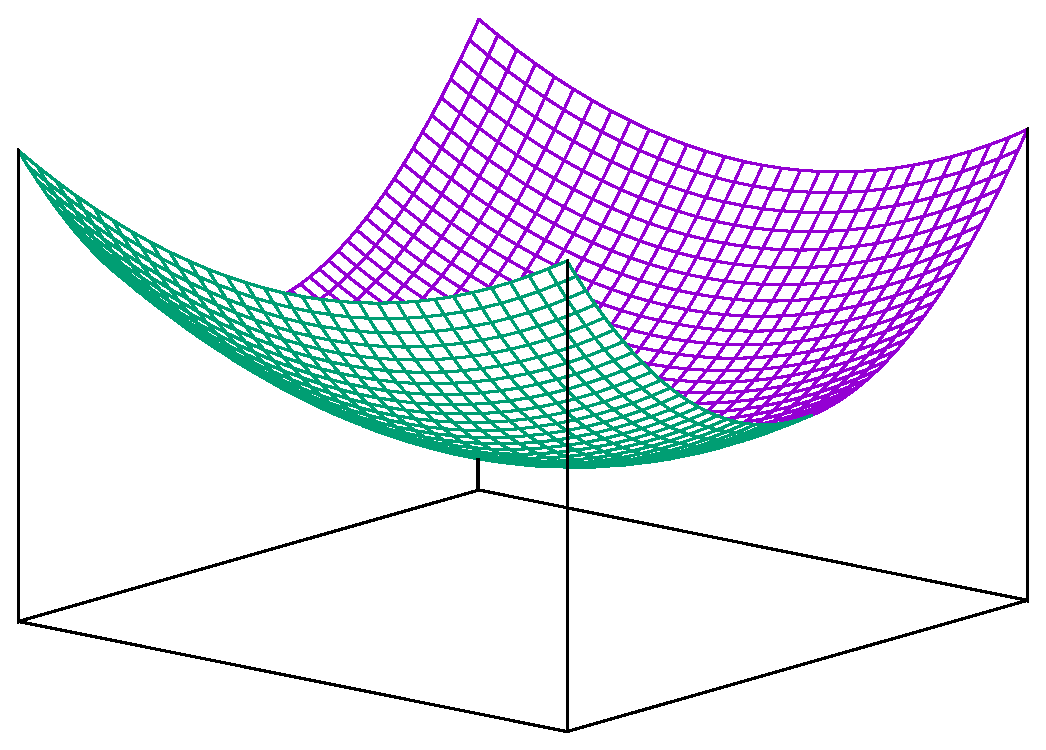
\includegraphics[scale=0.3]{eps/eliptico}
		\caption{El paraboloide elíptico.}
		\label{fig:eliptico}
\end{figure}
\end{example}

% FIXME: cambiar u por v en el helicoide
\begin{example}
	\label{exa:helicoide}
	\index{Helicoide}
	Sea $S$ el helicoide parametrizado por
	\[
		X(u,v)=(v\cos u,v\sin u,u),\quad
		u,v\in\R.
	\]
	Calculamos
	\begin{align*}
		& X_u=(-v\sin u,v\cos u,1),
		&& X_v=(\cos u,\sin u,0),\\
		& N_X=\frac{1}{\sqrt{1+v^2}}(-\sin u,\cos u,-v),
		&&X_{uu}=(-v\cos u,-v\sin u,0),\\
		&X_{uv}=(-\sin u,\cos u,0),
		&&X_{vv}=(0,0,0).
	\end{align*}
	Los coeficientes de las formas fundamentales son entonces
	\begin{align*}
		&E=1+v^2, && F=0, && G=1,
		&&e=g=0, && f=\frac{1}{\sqrt{1+v^2}}.
	\end{align*}
	Luego todo punto de $S$ es elíptico pues 
	\[
		K(X(u,v))=-\frac{1}{(1+v^2)^2}>0.
	\]
	Además $H(X(u,v))=0$. Podemos ver un gráfico de $S$ en la figura
\begin{lstlisting}
gnuplot> set parametric
gnuplot> set isosamples 50,30
gnuplot> set urange [-pi:pi]
gnuplot> set vrange [-pi:pi]
gnuplot> set hidd
gnuplot> unset xtics
gnuplot> unset ytics
gnuplot> unset ztics
gnuplot> set key off
gnuplot> set view 60,300
gnuplot> splot v*cos(u), v*sin(u), u
\end{lstlisting}
\begin{figure}
		\centering
    	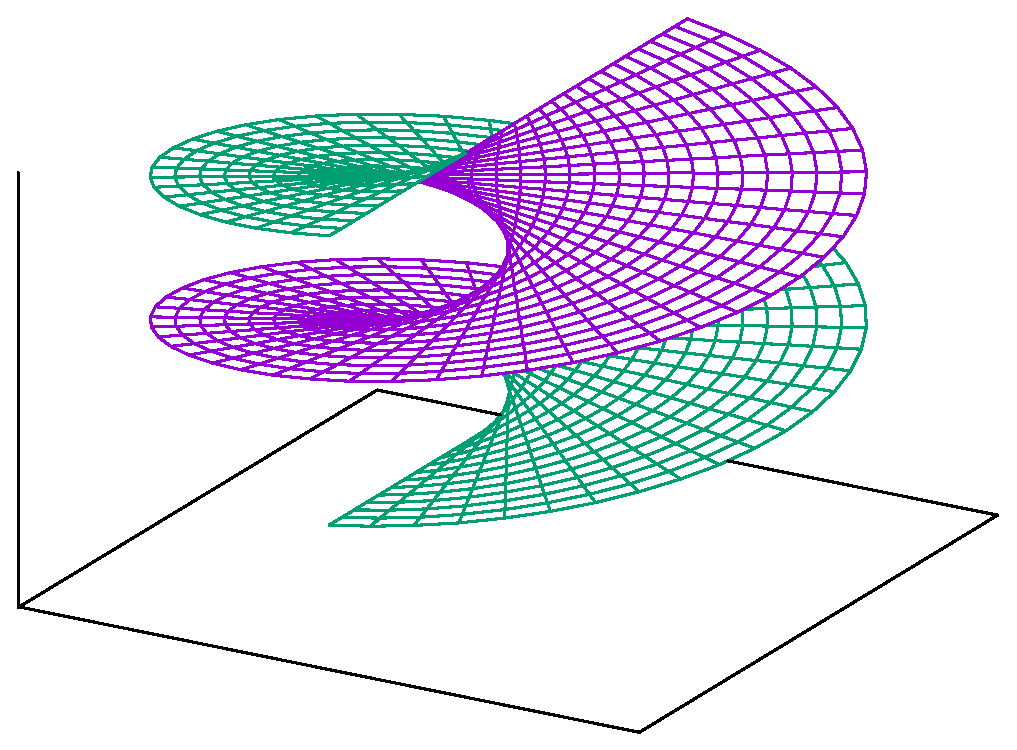
\includegraphics[scale=0.3]{eps/helicoide}
		\caption{El helicoide.}
		\label{fig:helicoide}
\end{figure}
\end{example}

\begin{example}
	Sea $S$ la superficie parametrizada por
	\[
		X(u,v)=(u,v,u^3-3v^2u).
	\]
	Veamos que el punto $X(0,0)$ es un punto plano. Primero calculamos
	\[
		X_u=(1,0,3(u^2-v^2)),\quad X_v=(0,1,-6vu)
	\]
	y luego $X_u(0,0)=(1,0,0)$, $X_v(0,0)=(0,1,0)$ y $N_X(0,0)=(0,0,1)$. Calculemos ahora
	\[
		X_{uu}=(0,0,6u),\quad
		X_{uv}=(0,0,-6v),\quad
		X_{vv}=(0,0,-6u)
	\]
	y entonces $X_{uu}(0,0)=X_{uv}(0,0)=X_{vv}(0,0)=(0,0,0)$. Los coeficientes
	de las forma fundamentales son entonces
	\[
		E(0,0)=G(0,0)=1,\quad
		F(0,0)=0,\quad
		e(0,0)=f(0,0)=g(0,0)=0.
	\]
	Luego $-(dN)_{X(0,0)}=0$ pues su matriz en la base $\{X_u(0,0),X_v(0,0)\}$ es 
	\[
		\frac{1}{EG-F^2}\begin{pmatrix}
			G & -F\\
			-F & E
		\end{pmatrix}
		\begin{pmatrix}
			e & f\\
			f & g
		\end{pmatrix}
		=\begin{pmatrix}
			0 & 0\\
			0 & 0
		\end{pmatrix}.
	\]
	El código 
\begin{lstlisting}
gnuplot> set parametric
gnuplot> set isosamples 50,30
gnuplot> set hidden3d
gnuplot> unset xtics
gnuplot> unset ytics
gnuplot> unset ztics
gnuplot> set key off
gnuplot> set view 75,125
gnuplot> splot u,v,u**3-3*v**2*u
\end{lstlisting}
produce el gráfico de $S$ que vemos en la figura~\ref{fig:monkey}. 
\begin{figure}
		\centering
    	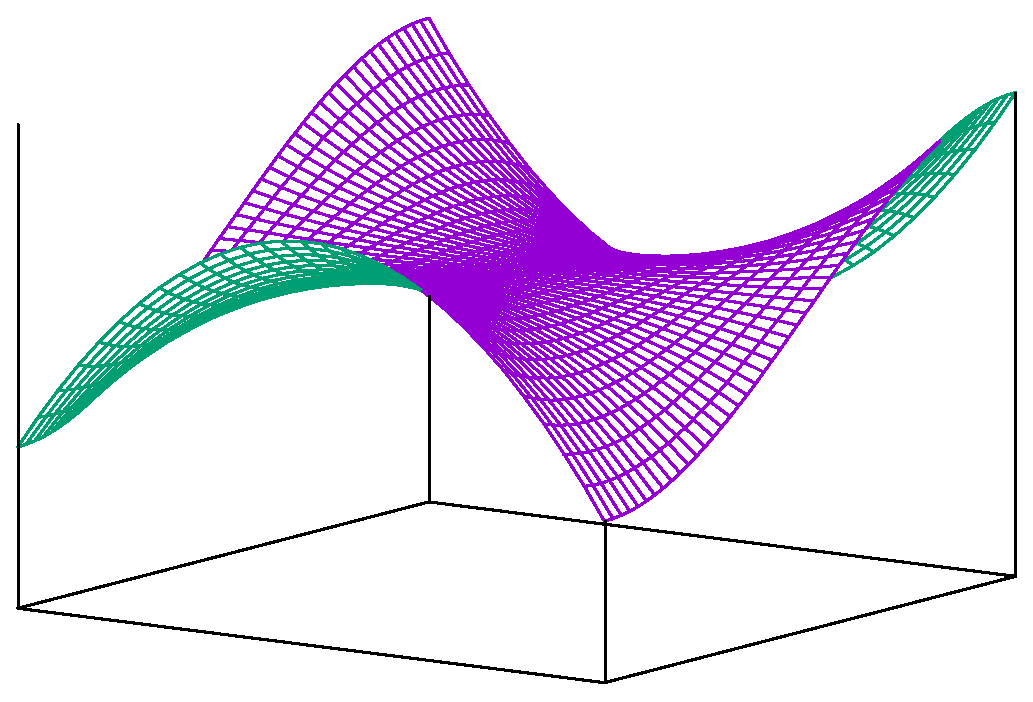
\includegraphics[scale=0.3]{eps/monkey}
		\caption{La silla de montar del mono.}
		\label{fig:monkey}
\end{figure}
\end{example}

\begin{example}[superficies de revolución]
	\index{Superficie!de revolución}
	\label{exa:revolucion}
	Sea $\gamma$ una curva regular sin autointersecciones contenida en el semiplano
	$\{(x,0,z)\in\R^3:x>0\}$, digamos
	\[
	\gamma(u)=(\sigma(u),0,\tau(u)),\quad u\in I.
	\]

	Vamos a considerar la superficie $S$ que se obtiene al rotar la
	\textbf{curva generatriz} $\gamma$ alrededor del eje $z$. Es decir, todo
	punto de $q\in S$ se obtiene de haber rotado en un ángulo $v$ un punto $p$
	de la imagen de $\gamma$ alrededor del eje $z$.

	Si $p=\gamma(u)=(\sigma(u),0,\tau(u))$ es un punto de la curva, entonces
	todo punto $q$ de la superficie $S$ puede escribirse como
	\[
		X(u,v)=(\sigma(u)\cos v,\sigma(u)\sin v,\tau(u)).
	\]

	Un cálculo sencillo muestra que
	\begin{align*}
		&X_u=(\sigma'(u)\cos v,\sigma'(u)\sin v,\tau'(u)),\\
		&X_v=(-\sigma(u)\sin v,\sigma(u)\cos v,0),\\
		&X_u\times X_v=(-\tau'(u)\sigma(u)\cos v,-\tau'(u)\sigma(u)\sin v,\sigma'(u)\sigma(u)),
	\end{align*}
	y luego 
	\[
		\|X_u\times X_v\|^2=\sigma^2(u)(\sigma'(u)^2+\tau'(u)^2)\ne 0
	\]
	 pues la curva $\gamma$ 
	es regular.
	Puede demostrarse fácilmente que $X\colon I\times(0,2\pi)\to\R^3$ es una
	parametrización. Esta parametrización no cubre la totalidad de la
	superficie de revolución pero si utilizamos otra parametrización similar a
	$X$, digamos por ejemplo
	\[
		Y\colon I\times(-\pi,2\pi)\to\R^3,\quad
		Y(u,v)=X(u,v),
	\]
	se concluye que $S$ es una superficie. 

	Calculemos los coeficientes de la primera forma fundamental:
	\[
		E(u,v)=\sigma'(u)^2+\tau'(u)^2,\quad
		F(u,v)=0,\quad
		G(u,v)=\sigma^2(u).
	\]
	Como 
	\begin{align*}
		&X_{uu}=(\sigma''(u)\cos v,\sigma''(u)\sin v,\tau''(u)),\\
		&X_{uv}=(-\sigma'(u)\sin v,\sigma'(u)\cos v,0),\\
		&X_{vv}=(-\sigma(u)\cos v,-\sigma(u)\sin v,0),
	\end{align*}
	y además $\|X_u\times X_v\|=\sqrt{EG-F^2}=\sigma(u)\sqrt{\sigma'(u)^2+\tau'(u)^2}$, los coeficientes de
	la segunda forma fundamental son
	\begin{align*}
		&e(u,v)=\frac{\tau''(u)\sigma'(u)-\sigma''(u)\tau'(u)}{\sqrt{\sigma'(u)^2+\tau'(u)^2}}=\frac{\det\begin{pmatrix}\sigma'(u) & \tau'(u)\\\sigma''(u)&\tau''(u)\end{pmatrix}}{\sqrt{\sigma'(u)^2+\tau'(u)^2}},\\
		&f(u,v)=0,\\
		&g(u,v)=\frac{\tau'(u)\sigma(u)}{\sqrt{\sigma'(u)^2+\tau'(u)^2}}.
	\end{align*}

	Como $F=f=0$, las curvaturas principales son entonces 
	\begin{align*}
		&\frac{e}{E}(u,v)=\frac{\tau''(u)\sigma'(u)-\sigma''(u)\tau'(u)}{(\sigma'(u)^2+\tau'(u)^2)^{3/2}}
%		=\frac{\det\begin{pmatrix}\sigma'(u) & \tau'(u)\\\sigma''(u)&\tau''(u)\end{pmatrix}}(\sigma'(u)^2+\tau'(u)^2)^{3/2}},\\
		&\frac{g}{G}(u,v)=\frac{\tau'(u)}{\sigma(u)\sqrt{\sigma'(u)^2+\tau'(u)^2}}
	\end{align*}
	y luego la curvatura gaussiana es
	\begin{align*}
		&K\circ X(u,v)=\frac{\tau'(\tau''\sigma'-\tau'\sigma'')}{\sigma (\sigma'^2+\tau'^2)^2 }(u).
%		&H\circ X=\frac12\frac{\tau'+\sigma(\tau''\sigma'-\sigma''\tau')}{\sigma}.
	\end{align*}
\end{example}

Lo hecho en el ejemplo anterior por supuesto nos da también una fórmula para la
curvatura media.  Si la curva $\gamma$ estuviera parametrizada por longitud de
arco, las fórmulas para las curvaturas quedarían mucho más sencillas.  En
efecto, si 
\[
\sigma'(u)^2+\tau'(u)^2=1
\]
para todo $u$, al derivar esta expresión, 
$\sigma'(u)\sigma''(u)+\tau'(u)\tau''(u)=0$. Al reemplazar esto en la
fórmula para la curvatura gaussiana se concluye que
\[
	K\circ X(u,v)=-\frac{\sigma''}{\sigma}(u).
\]

Veamos algunos ejemplos concretos de cálculo de curvaturas de superficies de
revolución. 
% catenaria pero parametrizada por longitud de arco

\begin{example}
	\index{Toro}
	Calculemos la curvatura gaussiana del toro que vemos en la
	figura~\ref{fig:toro} y que se obtiene de rotar la curva
	\[
		\sigma(u)=3+\cos u ,\quad
		\tau(u)=\sin u .
	\]
	Tal como hicimos en el ejemplo anterior consideramos la 
	parametrización
	\[
		X(u,v)=( (3+\cos u)\cos v,(3+\cos u)\sin v,\sin u).
	\]
	Como 
	\[
		\sigma'(u)=-\sin u,\quad
		\sigma''(u)=-\cos u,\quad
		\tau'(u)=\cos u,\quad
		\tau''(u)=-\sin u,
	\]
	vemos que $\sigma'(u)^2+\tau'(u)^2=1$ para todo $u$. 
	Las curvaturas son
	\[
		K = \frac{\cos u}{3+\cos u},
		\quad
		H = \frac{1}{2}\frac{3+2\cos u}{3+\cos u}.
	\]
	El código que produce la figura~\ref{fig:toro} es el siguiente:
\begin{lstlisting}
gnuplot> set parametric
gnuplot> set isosamples 50,30
gnuplot> set hidd
gnuplot> unset xtics
gnuplot> unset ytics
gnuplot> unset ztics
gnuplot> set key off
gnuplot> set view 36,16
gnuplot> splot [-pi:pi][-pi:pi] (3+cos(u))*cos(v),\
> (3+cos(u))*sin(v), sin(u)
\end{lstlisting}
\begin{figure}
		\centering
    	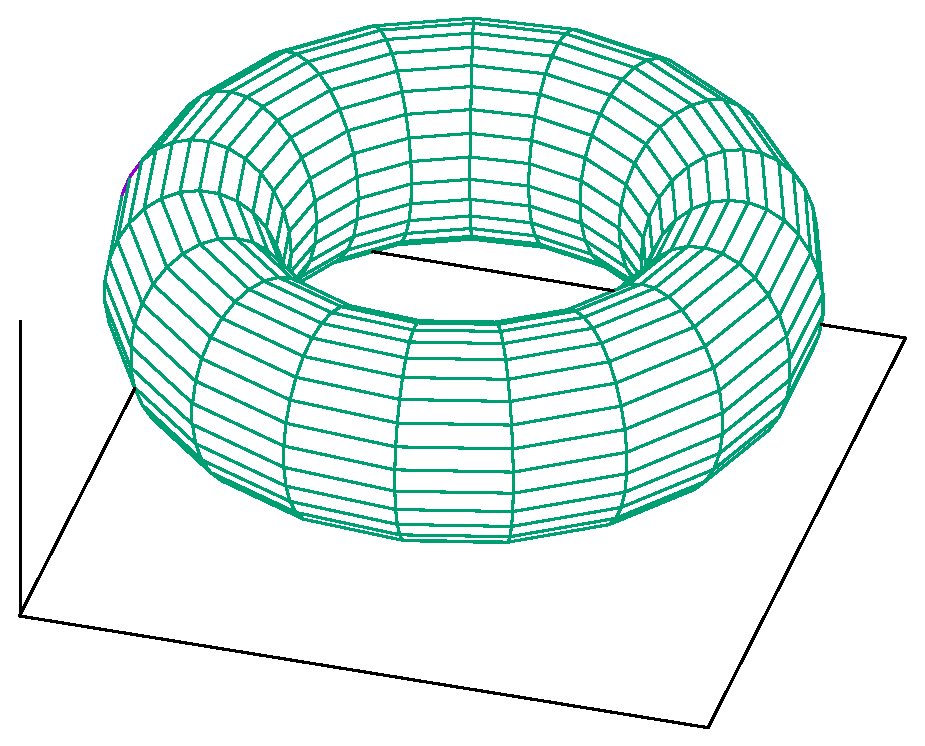
\includegraphics[scale=0.3]{eps/toro}
		\caption{El toro.}
		\label{fig:toro}
\end{figure}
\end{example}

\begin{example}
	\label{exa:catenoide}
	\index{Catenoide}
	Calculemos ahora las curvaturas del catenoide, que se obtiene de rotar la
	curva catenaria 
	\[
		\sigma(u)=\cosh u,\quad
		\tau(u)=u.
	\]
	Vemos en la figura~\ref{fig:catenoide} un gráfico de esta superficie de revolución.
	Consideremos la parametrización
	\[
		X(u,v)=(\cosh u \cos v ,\cosh u \sin v ,u).
	\]
	Calculamos:
	\[
		\sigma'(u)=\sinh u,\quad
		\sigma''(u)=\cosh u,\quad
		\tau'(u)=1,\quad
		\tau''(u)=0.
	\]
	Como $\sinh^2 u+1=\cosh^2 u$, al usar las fórmulas del ejemplo anterior 
	vemos que las curvaturas principales son entonces
	\[
		\frac{e}{E}=\frac{-1}{\cosh^2 u},\quad
		\frac{g}{G}=\frac{1}{\cosh^2 u}.
	\]
	Luego
	\begin{align*}
		&K\circ X(u,v)=\frac{-1}{\cosh^4 u},\\
		&H\circ X(u,v)=0.
	\end{align*}
	El código que produce la figura~\ref{fig:catenoide} es el siguiente:
\begin{lstlisting}
gnuplot> set parametric
gnuplot> set isosamples 50,30
gnuplot> set hidd
gnuplot> unset xtics
gnuplot> unset ytics
gnuplot> unset ztics
gnuplot> set key off
gnuplot> set view 70,200
gnuplot> splot cosh(u)*cos(v), cosh(u)*sin(v),u
\end{lstlisting}
\begin{figure}
		\centering
    	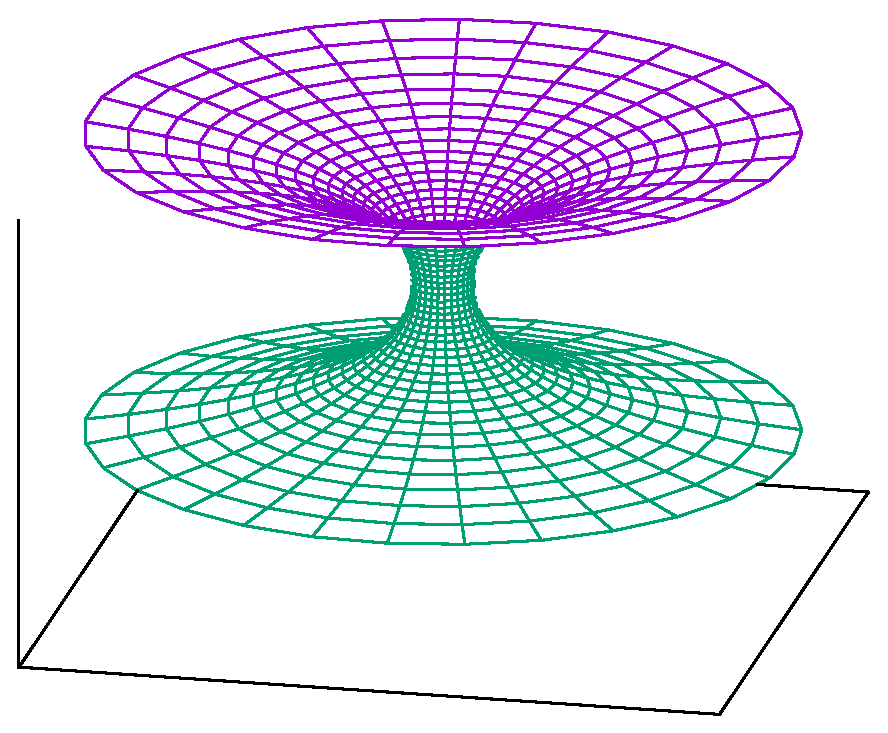
\includegraphics[scale=0.3]{eps/catenoide}
		\caption{La catenoide.}
		\label{fig:catenoide}
\end{figure}
\end{example}
	
% pag 272 oneill, caracterizacion de superficies minimas 
% curvatura prescripta positiva pag 275
% pseudoesfera 6.6, pagina 277

Para finalizar esta sección vamos a construir una superficie con curvatura
constante negativa. Comenzamos con una curva $\gamma(u)=(\sigma(u),\tau(u))$
parametrizada por longitud de arco. Consideramos la parametrización
\[
	X(u,v)=(\sigma(u)\cos v,\sigma(u)\sin v,\tau(u))
\]
de la superficie de revolución obtenida al rotar $\gamma$ alrededor del eje $z$. Sabemos
que la curvatura de esta superficie está dada por
\[
	K(X(u,v))=-\frac{\sigma''(u)}{\sigma(u)}
\]
Si queremos que nuestra superficie tenga curvatura constante igual a $-1$, entonces
$\sigma(u)=ae^u+be^{-u}$ para constantes $a,b\in\R$. Si suponemos que $a=1$ y $b=0$ y que $u\leq0$, entonces $\sigma(u)=e^u$ y luego,  
como $\sigma'(u)^2+\tau'(u)^2=1$, 
\[
	\tau(u)=\int\sqrt{1-e^{2u}}du.
\]
Si utilizamos la sustitución $\cos t=e^{u}$ y hacemos que la constante de integración sea igual a cero, obtenemos
\[
	\tau(u)=\sqrt{1-e^{2u}}-\log\left(e^{-u}+\sqrt{e^{-2u}-1}\right).
\]
Como $x=\sigma(u)$, $z=\tau(u)$ y $\cosh^{-1}v=\log(v+\sqrt{v^2-1})$, se concluye que
la curva $\gamma$ puede escribirse como
\[
	z=\sqrt{1-x^2}-\cosh^{-1}(1/x).
\]
\index{Pseudo-esfera}
\index{Tractriz}
La superficie que construimios puede verse en la figura~\ref{fig:pseudo} y se
conoce como \textbf{pseudo-esfera}.  

\begin{figure}
		\centering
    	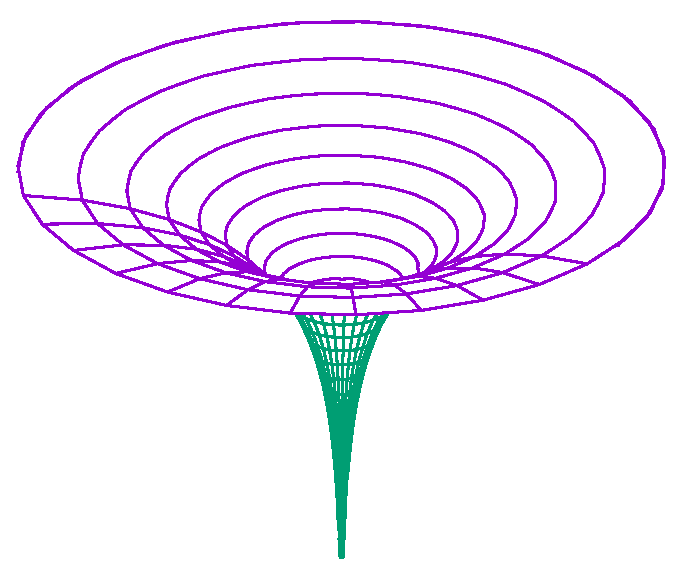
\includegraphics[scale=0.30]{eps/pseudo}
		\caption{La pseudo-esfera.}
		\label{fig:pseudo}
\end{figure}

La curva $\gamma$ que utilizamos para construir esta superficie de revolución
se conoce como la \textbf{tractriz} y puede verse en la
figura~\ref{fig:tractriz}.  

\begin{figure}
		\centering
    	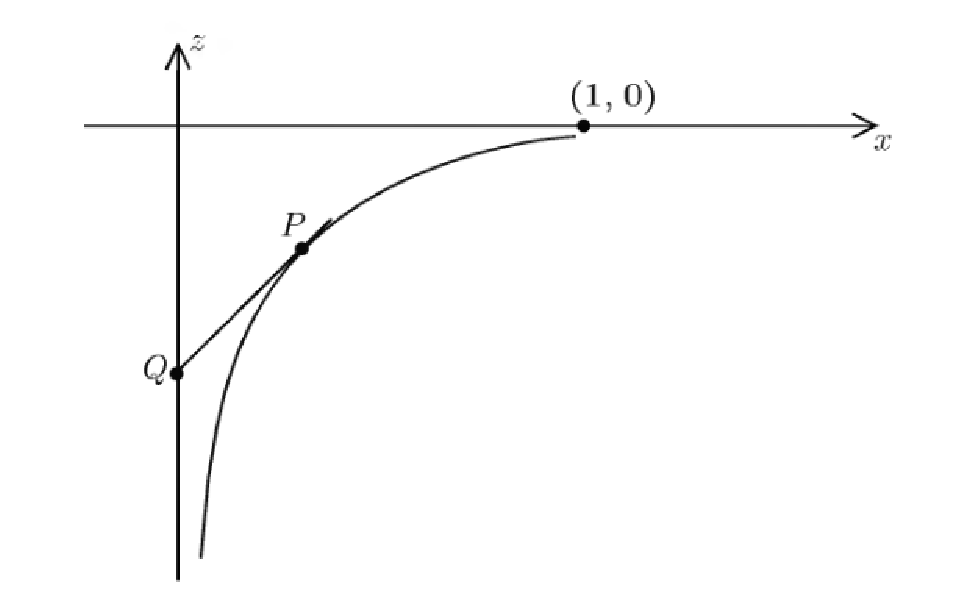
\includegraphics[scale=0.30]{eps/tractriz}
		\caption{La tractriz.}
		\label{fig:tractriz}
\end{figure}

Esta curva tiene una interesante propiedad
geométrica: Sea $P$ un punto de $\gamma$ y sea $Q$ la intersección entre la
tangente a $\gamma$ en $P$ y el eje $z$. Veamos que la distrancia entre $P$ y
$Q$ es constantemente igual a uno: si $P=(x_0,z_0)$, entonces
\[
	\frac{dz}{dx}=\frac{\sqrt{1-x^2}}{x}
\]
y luego la tangente en $P$ es
\[
	z-z_0=\frac{\sqrt{1-x_0^2}}{x_0}(x-x_0).
\]
Esta recta corta al eje $z$ en el punto $(0,z_1)$, donde
$z_1-z_0=-\sqrt{1-x_0^2}$. Luego la distancia entre $P$ y $Q$ es siempre igual
a $1$ pues $x_0^2+(z_1-z_0)^2=1$. La tractriz suele describirse así: Supongamos
que un nene tiene un autito atado con un cordon de longitud fija igual a a uno.
Si el nene está ubicado incialmente en $(0,0)$ el autito se ubicará en el punto
$(1,0)$. Si el nene camina sobre el eje $z$ en la dirección de los negativos,
el autito se moverá a lo largo de la tractriz. 

\begin{example}
	\index{Superficie!reglada}
	Otra familia de superficies de interés es la familia de superficies
	regladas. Una superficie se dirá \textbf{reglada} si puede escribirse como
	unión de líneas rectas. Una parametrización
	\[
		X(u,v)=\gamma(u)+v\delta(u)
	\]
	donde $\gamma$ y $\delta$ son curvas que cumplen ciertas condiciones que
	garantizan que $X$ sea la parametrización de una superficie. (Por ejemplo,
	el cono que vemos en la figura~\ref{fig:reglada} será una superficie
	siempre y cuando quitemos el origen de coordenadas.) Las líneas rectas de
	nuestra superficie serán $v\mapsto \gamma(u)+v\delta(u)$. 

	En la figura~\ref{fig:reglada} vemos algunos ejemplos de superficies
	regladas. La banda de M\"obius también es una superficie reglada.
	\begin{figure}
		\centering
    	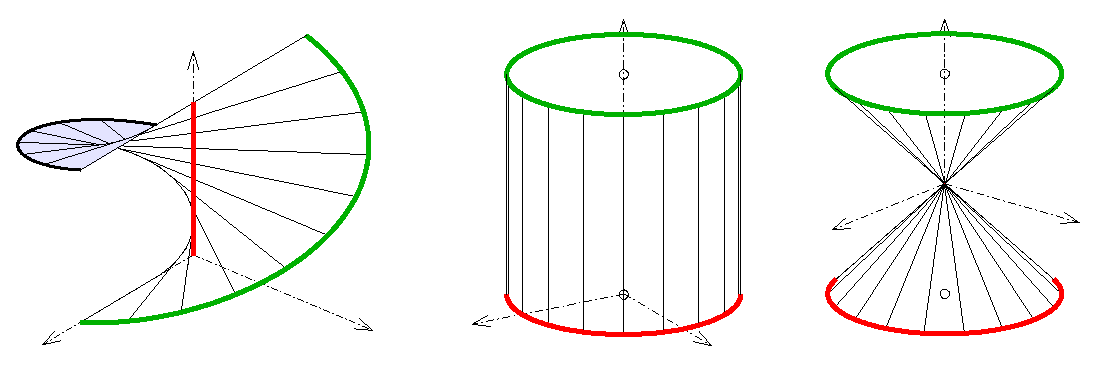
\includegraphics[scale=0.3]{eps/ruled}
		\caption{Algunas superficies regladas.}
		\label{fig:reglada}
	\end{figure}

	Supongamos que $X$ es la parametrización de una superficie reglada. 
	Calculamos
	\[
		X_u=\gamma'+v\delta',\quad
		X_v=\delta,\quad
		X_{uv}=\delta',\quad
		X_{vv}=0.
	\]
	Como $f=\langle \delta',N_X\rangle$ y $g=0$, se concluye entonces que 
	\[
		K=\frac{eg-f^2}{EG-F^2}=\frac{-\langle \delta',N_X\rangle}{EG-F^2}\leq 0.
	\]
\end{example}

\begin{example}
	\index{Cilindro!generalizado}
	Los \textbf{cilindros generalizados} son ejemplos de superficies regladas.
	Para definirlos necesitamos un vector unitario $a\in\R^3$ (y entonces
	$\delta(u)=a$ para todo $u$) y una curva $\gamma$ parametrizada por
	longitud de arco tal que $\langle\gamma(u),a\rangle=0$ para todo $u$. En
	ese caso 
	\[
		X(u,v)=\gamma(u)+va
	\]
	parametriza una superficie. Los coeficientes de la primera forma
	fundamental son $E=G=1$ y $F=0$. Como $\delta'=0$, el ejemplo anterior nos
	dice que la curvatura de Gauss es identicamente nula.
\end{example}

\chapter{El teorema de Hilbert}

Veremos ahora tres teoremas de rigidez de esferas. Básicamente son teoremas que
nos dicen que si alguna superficie, desde cierto punto de vista se parece a una
esfera, es entonces una esfera. 

% explicar mejor por qué podemos pensar que la superficie es localemente el gráfico de una función
% puede usarse el teorema de la función inversa para superficies

\begin{theorem}[Hilbert]
	\index{Teorema!de Hilbert}
	Sea $S$ una superficie orientada. Si existe un punto $p\in S$ tal que
	$K(p)>0$, $k_1(p)$ es un máximo local para $k_1$ y $k_2(p)$ es un mínimo
	local para $k_2$, entonces el punto $p$ es umbílico.
\end{theorem}

\begin{proof}
	Después de aplicar un movimiento rígido si fuera necesario, podemos 
	suponer que $p=(0,0,0)$, que las direcciones principales son
	\[
		e_1=(1,0,0),\quad
		e_2=(0,1,0),
	\]
	y que $N(p)=(0,0,1)$. 
	En un entorno suficientemente pequeño de $p$, $S$ es el gráfico de una función
	$h$. Sea $X\colon U\to S$, $X(u,v)=(u,v,h(u,v))$, una
	parametrización alrededor de $p$ tal que $X(0,0)=p$. Entonces
	\[
		X_u(0,0)=(1,0,h_u(0,0)),\quad
		X_v(0,0)=(0,1,h_v(0,0)).
	\]
	Si escribimos $X_u(0,0)=e_1+\lambda N(p)$ para algún $\lambda\in\R$,
	entonces $0=\langle X_u(0,0),N(p)\rangle$ implica que $\lambda=0$ y luego
	$h_u(0,0)=0$. Análogamente vemos que $h_v(0,0)=0$,
	\[
		X_u(0,0)=(1,0,0)=e_1,\quad
		X_v(0,0)=(0,1,0)=e_2.
	\]
	Como $X(U)$ es el gráfico de una función $h$, 
	los coeficientes de la segunda forma fundamental en $X(0,0)$ son
	\[
		e=\frac{h_{uu}}{\sqrt{1+h_u^2+h_v^2}},\quad
		f=\frac{h_{uv}}{\sqrt{1+h_u^2+h_v^2}},\quad
		g=\frac{h_{vv}}{\sqrt{1+h_u^2+h_v^2}}.
	\]
	Luego, como por otro lado, 
	\begin{align*}
		&e=\langle -(dN)_p(X_u),X_u\rangle=k_1(p),\\
		&f=\langle -(dN)_p(X_u),X_v\rangle=0,\\
		&g=\langle -(dN)_p(X_v),X_v\rangle=k_2(p),
	\end{align*}
	se concluye que 
	\[
		h_{uu}(0,0)=k_1(p),\quad
		h_{uv}(0,0)=0,\quad
		h_{vv}(0,0)=k_2(p).
	\]
	Sea $\alpha,\beta\colon U\to S$ las curvas en $S$ dadas por
	\[
		\alpha(u)=X(u,0),\quad
		\beta(v)=X(0,v)
	\]
	y sean $A,B\colon U\to\R^3$ las curvas dadas por
	\[
		A(u)=\frac{1}{\|X_v(u,0)\|}X_v(u,0),\quad
		B(v)=\frac{1}{\|X_u(0,v)\|}X_u(0,v).
	\]

	Sean
	\begin{align*}
		a(u) &= \II_{\alpha(u)}(A(u))=\frac{1}{1+h_v^2}\frac{h_{vv}}{\sqrt{1+h_u^2+h_v^2}}(u,0),\\
		b(v) &= \II_{\beta(v)}(B(v))=\frac{1}{1+h_u^2}\frac{h_{uu}}{\sqrt{1+h_u^2+h_v^2}}(0,v).
	\end{align*}
	Como por hipótesis $k_2(p)$ es un mínimo local para $k_2$, el teorema de
	Meusnier y la fórmula de Euler implican que  
	\[
		a(0)=h_{vv}(0,0)=k_2(p)\geq k_2(\alpha(u))\leq\II_{\alpha(u)}A(u)=a(u).
	\]
	Análogamente, como $k_1(p)$ es un máximo local para $k_1$, 
	\[
		b(0)=h_{uu}(0,0)=k_1(p)\leq k_1(\beta(v))\geq\II_{\beta(v)}B(v)=b(v).
	\]
	Como entonces $a(u)$ tiene un máximo local en $u=0$ y $b(v)$ tiene un
	mínimo local en $v=0$, 
	\[
		b''(0)\leq 0 \leq a''(0).
	\]
%	Calculemos ahora estas derivadas. Primero:
%	\begin{align*}
%		a'(u) = -2(1+h_v^2)^{-2}&h_vh_{uv}(1+h_u^2+h_v^2)^{-1/2}h_{vv}\\
%		&-\frac12(1+h_v^2)^{-1}(1+h_u^2+h_v^2)^{-3/2}(2h_uh_{uu}+2h_vh_{uv})h_vv\\
%		&+(1+h_v^2)^{-1}(1+h_u^2+h_v^2)^{-1/2}h_{vvu}.
%	\end{align*}
%	Después:
%	\begin{align*}
%		a''(0)=\dots
%	\end{align*}
	Un cálculo sencillo y tedioso nos muestra que
	\begin{align*}
		&a''(0)=-h_{uu}^2(0,0)h_{vv}(0,0)+h_{vvuu}(0,0),\\
		&b''(0)=-h_{vv}^2(0,0)h_{uu}(0,0)+h_{uuvv}(0,0).
	\end{align*}
	Como $h_{vvuu}(0,0)=h_{uuvv}(0,0)$, $K(p)>0$ y $k_1(p)\geq k_2(p)$ por
	hipótesis, entonces 
	\begin{align*}
		0 & \leq b''(0)-a''(0)\\
		&= h_{uu}(0,0)h_{vv}(0,0)(h_{uu}(0,0)-h_{vv}(0,0))
		= K(p)(k_1(p)-k_2(p))\leq 0.
	\end{align*}
	Luego $k_1(p)=k_2(p)$.
\end{proof}

% toda superficie es localemente un gráfico
% calcular curvatura en gráficos

Veamos algunos corolarios:

\begin{theorem}[Jellet--Liebmann]
	\index{Teorema!de Jellet--Liebmann}
	Toda superficie orientable compacta y conexa con curvatura gaussiana positiva 
	y curvatura media constante es una esfera.
\end{theorem}

\begin{proof}
%	La curvatura media $H$ es una constante, digamos $c$. Si $c=0$, entonces
%	$k_1=-k_2$ y luego $K(p)=-k_1(p)^2\leq 0$ para todo $p$, una contradicción. 
%
	Como las curvaturas princiaples $k_1,k_2\colon S\to\R$ son funciones
	continuas y $S$ es compacto, existe $p\in S$ donde $k_1$ alcanza su máximo.
	Como $k_2=2c-k_1$, entonces $k_2$ alcanza su mínimo en ese mismo punto $p$.
	Por el teorema de Hilbert, $p$ es entonces un punto umbílico.  Si $q\in S$,
	entonces
	\[
		k_2(q)\leq k_1(q)\leq k_1(p)=k_2(p)\leq k_2(q)
	\]
	y luego $k_1(q)=k_2(q)$ para todo $q\in S$. Como todo punto es entonces
	umbílico y $S$ es compacto, $S$ es una esfera por el
	teorema~\ref{thm:es_esfera}.
\end{proof}

\index{Teorema!de Brouwer--Samelson}
En el teorema anterior tuvimos que suponer que la superficie es orientable para
tener definida la curvatura media en todo punto. Puede omitirse esta hipótesis
al observar que toda superficie con curvatura gaussiana positiva en todo punto
es orientable. Como alternativa podría usarse el teorema de Brouwer--Samelson,
que afirma que toda superficie compacta es orientable. Una demostración de este
resultado puede verse en ~\cite[Theorem 4.16]{MR2522595} o bien
en~\cite[Theorem 4.7.15]{MR2964051}.

\begin{theorem}[Hilbert--Liebmann]
	\index{Teorema!de Hilbert--Liebmann}
	Toda superficie orientable, compacta y conexa con curvatura gaussiana
	constante es una esfera.
\end{theorem}

\begin{proof}
	La demostración es similar a la del teorema anterior. 
	Si $K$ es una constante $c$, entonces $c>0$ (pues por el 
	teorema~\ref{thm:compacta_eliptico} sabemos que $S$ 
	tiene al menos un punto de curvatura positiva).  
	La clave ahora es observar que $k_2(p)=c/k_1(p)$ y que, como 
	que si $k_1$ alcanza un mínimo en un punto, ese punto será un máximo para
	$k_2$ pues $k_2$ puede escribirse como una función decreciente en $k_1$.
	%Vimos en el teorema~\ref{thm:compacta_eliptico} que toda superficie
	%compacta tiene al menos un punto de curvatura positiva. Luego la curvatura
	%de nuestra superficie $S$ es siempre positiva por ser constante.  Como
	%hicimos en el teorema anterior, $k_1$ alcanzará un mínimo en un punto
	%$q\in S$ y luego $q$ será un máximo para $k_2$. Por el teorema de
	%Hilbert, para todo $p\in S$, 
	%\[
	%	k_2(p)\leq k_2(q)=k_1(q)\leq k_1(p)
	%\]
	%y luego todo punto de $S$ es umbílico. Se concluye que $S$ es entonces una
	%esfera.
\end{proof}

El argumento utilizado para demostrar los teoremas anteriores da otros
resultados similares. Puede demostrarse por ejemplo que toda superficie conexa
y compacta de curvatura positiva y tal que $K/H$ es constante es necesariamente
una esfera. 

\chapter{Isometrías y aplicaciones conformes}

%\index{Difeomorfismo local}
%Una función diferenciable $f\colon S\to T$ entre superficies será un
%\textbf{difeomorfismo local} si para cada $p\in S$ existe un abierto $U$ que
%contiene a $p$ tal que $f(U)$ es abierto en $T$ y la restricción $f|_U\colon
%U\to f(U)$ es un difeomorfismo.

\index{Isometría local}
Diremos que una función diferenciable $f\colon S\to T$ entre superficies es una
\textbf{isometría local} si para cada $p\in S$, 
\[
\langle (df)_p(v),(df)_p(w)\rangle=\langle v,w\rangle
\]
para todo $v,w\in T_pS$. 

Recordemos que si transformación lineal $T\colon V\to W$ entonces $\langle
Tx,Ty\rangle=\langle x,y\rangle$ para todo $x,y\in V$ si y sólo si
$\|Tx\|=\|x\|$ para todo $x\in V$. 

\begin{lemma}
	\label{lem:longitud_curvas}
	Una función diferenciable $f\colon S\to T$ es una isometría local si y sólo
	si $f$ preserva la longitud de las curvas.	
\end{lemma}

\begin{proof}
	Sea $\alpha$ una curva en $S$. 
	Supongamos que $f$ es una isometría local. Como
	\[
		\|(f\circ\alpha)'(t)\|=\|(df)_{\alpha(t)}(\alpha'(t))\|=\|\alpha'(t)\|,
	\]
	se concluye que $\alpha$ y $f\circ\alpha$ tienen la misma longitud pues 
	\[
		L_a^b(f\circ\alpha)=\int_a^b\|(f\circ\alpha)'(t)\|dt=\int_a^b\|\alpha'(t)\|dt=L_a^b(\alpha).
	\]

	Supongamos ahora que $f$ preserva la longitud de curvas. Sea $p\in S$ y sea $v\in T_pS$. Si $\alpha$ es una curva en $S$ 
	tal que $\alpha(0)=p$ y $\alpha'(0)=v$, entonces
	\[
		\int_0^t\|(f\circ\alpha)'(u)\|du=L_0^t(f\circ\alpha)=L_0^t(\alpha)=\int_0^t\|\alpha'(u)\|du.
	\]
	Al derivar esta expresión con respecto a $t$ y usar el teorema fundamental
	del cálculo, 
	\[
		\|(df)_p(v)\|=\|(f\circ\alpha)'(t)\|=\|v\|,
	\]
	que como $v$ es arbitrario, es equivalente a decir que
	$\langle(df)_pv,(df)_pw\rangle=\langle v,w\rangle$.
\end{proof}

Del lema anterior puede obtenerse fácilmente el siguiente hecho: una función
$f$ es una isometría local si y sólo si $\|(f\circ\alpha)'\|=\|\alpha'\|$ para
toda curva $\alpha$. 

\begin{example}
	Sea 
	\[
		S=\{(x,y,z)\in\R^3:x^2+y^2=z^2\}\cap\{(x,y,z)\in\R^3:z>0\}.
	\]
	La función $f\colon S\to\R^3$, $f(x,y,z)=(x,y,0)$, no es una isometría
	local. La longitud de la curva $\alpha(t)=(t,0,t)$ en $[1,2]$ es igual a
	\[
		L_1^2(\alpha)=\int_1^2\|\alpha'(t)\|dt=\sqrt{2}.
	\]
	En cambio, como $f(\alpha(t))=(t,0,0)$, la longitud de $f\circ\alpha$ es 
	\[
		\int_1^2\|(1,0,0)\|dt=1.
	\]
\end{example}

\index{Difeomorfismo local}
Una función diferenciable $f\colon S\to T$ entre dos superficies es un
\textbf{difeomoerfismo local} si para cada $p\in S$ existe un entorno $V$ de
$p$ en $S$ tal que $f(V)$ es un abierto de $T$ y la restricción $f|_V\colon
V\to f(V)$ es un difeomorfismo.

\begin{proposition}
	Si $f$ es una isometría local, entonces $f$ es un difeomorfismo local.
\end{proposition}

\begin{proof}
	Si existe algún $p\in S$ tal que $(df)_p$ no es inversible, existe $0\ne
	v\in T_pS$ tal que $(df)_p(v)=0$. Luego
	\[
		0\ne\langle v,v\rangle=\langle (df)_p(v),(df)_p(v)\rangle=0,
	\]
	una contradicción.
\end{proof}

\begin{lemma}
	\label{lem:isometria_local}
	Sea $f\colon S\to T$ un difeomorfismo local. Entonces 
	$f$ es una isometría local si y sólo si para cada parametrización $X$ de $S$ 
	las primeras formas fundamentales de $X$ y $Y=f\circ X$ coinciden.
\end{lemma}

\begin{proof}
	Como $Y=f\circ X$, la regla de la cadena implica que 
	\[
		Y_u = (df)_X(X_u),\quad
		Y_v = (df)_X(X_v).
	\]
	Vemos entonces que $f$ es una isometría local si y sólo si 
	\[
		\langle X_u,X_u\rangle=\langle Y_u,Y_u\rangle,
		\quad
		\langle X_u,X_v\rangle=\langle Y_u,Y_v\rangle,
		\quad
		\langle X_v,X_v\rangle=\langle Y_v,Y_v\rangle.\qedhere
	\]
\end{proof}

%Diremos que un concepto geométrico es \textbf{intrínsico} si es invariante por
%isometrías, es decir si depende solamente de la primera forma fundamental.
%	
%Diremos que dos superficies $S$ y $T$ son \textbf{isométricas} si existe un
%difeomorfismo $f\colon S\to T$ que transforma cada curva de $S$ en una curva de
%$T$ de la misma longitud. Una tal $f$ se llama \textbf{isometría}.

\begin{example}
	\index{Plano}
	\index{Cilindro}
	El plano y el cilindro son localmente isométricos. El plano de ecuación
	$z=0$ puede parametrizarse como $X(u,v)=(u,v,0)$ y el cilindro como
	$Y(u,v)=(\cos u,\sin u,v)$. Como
	\[
		X_u=(1,0,0),\quad
		X_v=(0,1,0),\quad
		Y_u=(-\sin u,\cos u,0),\quad
		Y_v=(0,0,1),
	\]
	se tiene que el plano y el cilindro son localmente isométricos pues en
	ambos casos $E=G=1$ y $F=0$.
\end{example}

\begin{example}
	\index{Helicoide}
	\index{Catenoide}
	Veamos que el helicoide y la catenoide son superficies localmente
	isométricas. 
	Para la catenoide:
	\[
		Y(u,v)=(\cosh u\cos v,\cosh u\sin v,u),\quad v\in(0,2\pi).
	\]
	En el ejemplo~\ref{exa:catenoide} calculamos los coeficientes de la primera
	forma fundamental:
	\[
		E=G=\cosh^2 u,\quad
		F=0.
	\]

	Para el helicoide usamos la parametrización
	\[
		X(\overline{u},\overline{v})=(\overline{v}\cos\overline{u},\overline{v}\sin\overline{u},\overline{u}),\quad \overline{u}\in(0,2\pi).
	\]
	El cambio de variables 
	\[
	\begin{cases}
		\overline{u}=v,\\
		\overline{v}=\sinh u
	\end{cases},
	\]
	tiene jacobiano igual a 
	\[
		\frac{\partial(\overline{u},\overline{v})}{\partial(u,v)}
		=\det\begin{pmatrix}
			0 & 1\\
			\cosh u & 0
		\end{pmatrix}=-\cosh u\ne 0.
	\]
	Entonces, como
	\[
		X(u,v)=X(v,\sinh u)=(\sinh u\cos v,\sinh u\sin v,v),
	\]
	se tiene que 
	\begin{align*}
		&X_u=(\cosh u\cos v,\cosh u\sin v,0), &&
		X_v=(-\sinh u\sin v,\sinh u\cos v,1).
	\end{align*}
	y luego
	$E=G=\cosh^2 u$ y $F=0$. Esto nos dice que la función $(u,v)\mapsto
	(v,\sinh u)$ es una isometría local entre el helicoide y la catenoide. 
\end{example}

\index{Aplicación!conforme}
\index{Ángulo!entre curvas}
Nos interesa ahora estudiar funciones que preservan ángulos entre curvas. ¿Cómo
definimos ángulos entre curvas? Simplemente usando la geometría del espacio
tangente: el ángulo entre dos curvas $\gamma_1$ y $\gamma_2$ que se
cortan en el punto $p=\gamma_1(0)=\gamma_2(0)$ es por definición el ángulo que
forman los vectores tangente $\gamma_1'(0)$ y $\gamma_2'(0)$.  Un difeomorfismo
local $f\colon S\to T$ se dirá \textbf{conforme} si 
$f$ preserva ángulos. 

El ángulo $\theta$ formado por las curvas regulares $\gamma_1$ y $\gamma_2$ en
el punto $p=\gamma_1(0)=\gamma_2(0)$ está definido por
\[
	\cos\theta=\frac{\langle \gamma_1'(0),\gamma_2'(0)\rangle}{\|\gamma_1'(0)\|\|\gamma_2'(0)\|}.
\]
Para que $f$ preserve ángulos necesitamos que las curvas $f\circ\gamma_1$ y
$f\circ\gamma_2$ también sean regulares (y así podremos calcular el ángulo que
forman), y es por eso que pedimos que $f$ sea un difeomorfismo local.

Si $X$ es una parametrización de $S$ en $p$ tal que $p=X(0,0)$ y escribimos a
cada $\gamma_j$ en coordenadas, digamos 
$\gamma_1(t)=X(u_1(t),v_1(t))$ y 
$\gamma_2(t)=X(u_2(t),v_2(t))$, 
entonces 
\[
\gamma_j'(0)=X_u(0,0)u_j'(0)+X_v(0,0)v_j'(0)
\]
para $j\in\{1,2\}$. Luego
\[
	\cos\theta=\frac{Eu_1'u_2'+F(u_1'v_2'+u_2'v_1')+Gv_1'v_2'}{\sqrt{Eu_1^2+2Fu_1v_1+Gv_1^2}\sqrt{Eu_2^2+2Fu_2v_2+Gv_2^2}}.
\]

\begin{lemma}
	Sea $f\colon S\to T$ un difeomorfismo local. Entonces $f$ es conforme si y
	sólo si existe una función $\lambda\colon S\to\R$ tal que 
	\[
		\langle (df)_p(v),(df)_p(w)\rangle=\lambda(p)\langle v,w\rangle
	\]
	para todo $v,w\in T_pS$. 
\end{lemma}

\begin{proof}
	Demostremos primero la implicación $\Longleftarrow$. 
	Si $\gamma_1$ y $\gamma_2$ son curvas en $S$ tales que $p=\gamma_1(0)=\gamma_2(0)$ y $\theta$ es el ángulo que forman en $p$, calculamos
	\begin{align*}
		\langle (f\circ\gamma_i)'(0),(f\circ\gamma_j)'(0)\rangle
		&=\langle (df)_p(\gamma_i'(0),(df)_p(\gamma_j(0)\rangle=\lambda(p)\langle \gamma_i'(0),\gamma_j'(0)\rangle
	\end{align*}
	para cada $i,j\in\{1,2\}$. En particular,
	\begin{align*}
		\frac{\langle (f\circ\gamma_1)'(0),(f\circ\gamma_2)'(0)\rangle}{\|(f\circ\gamma_1)'(0)\|\|(f\circ\gamma_2)'(0)\|}
		&=\lambda(p)\frac{\langle \gamma_1'(0),\gamma_2'(0)\rangle}{\sqrt{\lambda(p)}\|\gamma_1'(0)\|\sqrt{\lambda(p)}\|\gamma_2'(0)\|}\\
		&=\frac{\langle \gamma_1'(0),\gamma_2'(0)\rangle}{\|\gamma_1'(0)\|\|\gamma_2'(0)\|}
	\end{align*}
	y luego $f$ es conforme. 

	Recíprocamente, sea $\{v_1,v_2\}$ una base ortonormal de $T_pS$ y sean
	\begin{align*}
		\lambda_1&=\langle (df)_p(v_1),(df)_p(v_1)\rangle,\\
		\lambda_2&=\langle (df)_p(v_1),(df)_p(v_2)\rangle,\\
		\lambda_3&=\langle (df)_p(v_2),(df)_p(v_2)\rangle.
	\end{align*}
	Por hipótesis, 
	\[
		\frac{\langle v,w\rangle}{\|v\|\|w\|}=\frac{\langle (df)_p(v),(df)_p(w)\rangle}{\|(df)_p(v)\|\|(df)_p(w)\|}
	\]
	para todo $v,w\in T_pS$. En particular, si $v=v_1$ y $w=(\cos \theta)v_1+(\sin\theta)v_2$, entonces
	\[
		\cos\theta=\frac{\cos\theta\lambda_1+\sin\theta\lambda_2}{\sqrt{\lambda_1(\cos^2\theta\lambda_1+2\cos\theta\sin\theta\lambda_2+\sin^2\theta\lambda_3}}
	\]
	para todo $\theta$. Si $\theta=\pi/2$ obtenemos $\lambda_2=0$ y luego 
	\[
		\lambda_1\cos^2\theta+\lambda_3\sin^2\theta=\lambda_1
	\]
	para todo $\theta$. Si ahora $\theta=0$, se concluye entonces que $\lambda_1=\lambda_3$. Con $\lambda=\lambda_1$, obtenemos
	\[
		\langle (df)_p(v),(df)_p(w)\rangle=\lambda\langle v,w\rangle
	\]
	para todo $v,w\in T_pS$.
\end{proof}

\begin{example}
	Sea $X$ una parametrización de una superficie $S$ y sea $p=X(0,0)\in S$. Para 
	las curvas $\gamma_1(t)=X(0,t)$ y $\gamma_2(t)=X(t,0)$ tenemos
	\[
		u_1(t)=0,\quad
		v_1(t)=t,\quad
		u_2(t)=t,\quad
		v_2(t)=0.
	\]
	Como entonces $u_1'(t)=v_2'(t)=0$ y $u_2'(t)=v_1'(t)=1$, el ángulo $\theta$ formado por las curvas
	$\gamma_1$ y $\gamma_2$ en el punto $p=\gamma_1(0)=\gamma_2(0)$ cumple
	\[
		\cos\theta=\frac{F}{\sqrt{EG}}(0,0).
	\]
\end{example}

\index{Proyección esterográfica}
Un ejemplo famoso de aplicación conforme está dado por la \textbf{proyección
estereográfica}. Consideremos la esfera unitaria $S^2$ con centro en $(0,0,0)$
y sea $N=(0,0,1)$ el polo norte.  Cada punto de $S^2\setminus\{N\}$ se
corresponde biyectivamente con un punto del plano $z=0$. En efecto, la línea
recta que une $N$ con $q$ corta el plano $z=0$ en el punto $p$. Queda definida
entonces la \textbf{proyección estereográfica}
\[
	\Pi\colon S^2\setminus\{N\}\to\{(x,y,z)\in\R^3:z=0\},
	\quad
	q\mapsto p.
\]

\begin{theorem}
	\label{thm:estereografica}
	\index{Proyección estereográfica}
	La proyección esterográfica $\Pi$ es conforme.
\end{theorem}

\begin{proof}
	Vamos a encontrar una parametrización de la esfera $S^2$ sin el polo norte
	$N=(0,0,1)$.  Dado un punto $q=(x,y,z)$ de la esfera, trazamos la recta $L$
	que une $N$ con $q$. Esta recta $L$ corta al plano de ecuación $z=0$ en un
	punto $p=(u,v,0)$. Sea
	\[
		\Pi(a,b,c)=(u,v).
	\]
	
	La ecuación de la recta $L$ es $q-N=N+\lambda(p-N)$, es decir:
	\begin{align*}
		x=\lambda u,&&
		y=\lambda v,&&
		z=1-\lambda.
	\end{align*}
	Como $z\ne 1$,
	\[
		\Pi(x,y,z)=(u,v,0)=\left(\frac{x}{1-z},\frac{y}{1-z},0\right).
	\]
	Como $x^2+y^2+z^2=1$, entonces
	$(\lambda u)^2+(\lambda v)^2+(1-\lambda)^2=1$ 
	y luego
	\[
		\lambda=\frac{2}{u^2+v^2+1},\quad
		q=\left(\frac{2u}{u^2+v^2+1},\frac{2v}{u^2+v^2+1},\frac{u^2+v^2-1}{u^2+v^2+1}\right).
	\]
	Tenemos entonces una parametrización de $S^2\setminus\{N\}$ dada por 
	\[
		X(u,v)=
		\left(\frac{2u}{u^2+v^2+1},\frac{2v}{u^2+v^2+1},\frac{u^2+v^2-1}{u^2+v^2+1}\right).
	\]
	Si parametrizamos al plano $z=0$ como $Y(u,v)=(u,v,0)$, vemos entonces que
	$\Pi(X(u,v))=Y(u,v)$. Sabemos que los coeficientes de la primera forma
	fundamental con respecto a $Y$ son $E=G=1$ y $F=0$. Para $\Pi\circ X$ son 
	\[
		E=G=\frac{4}{(u^2+v^2+1)^2},\quad 
		F=0.
	\]
	Si $\lambda=4/(u^2+v^2+1)^2$, entonces las primeras formas fundamentales
	son proporcionales y luego $\Pi$ es conforme. 
\end{proof}

A continuación veremos otros dos ejemplos importante de aplicación conforme, ambos
relacionados con superficies mínimas. Para el primero de estos ejemplos
recordemos el siguiente caso particular del teorema de Cayley--Hamilton: toda
matriz
$A=\left(\begin{smallmatrix}a&b\\c&d\end{smallmatrix}\right)\in\R^{2\times 2}$
es raíz del polinomio \[X^2-(a+d)A+(ad-bc)I=0.\]

\begin{theorem}
	Si $S$ es una superficie mínima con curvatura de Gauss no nula, entonces
	$N$ es conforme.
\end{theorem}

\begin{proof}
	Sabemos que $N$ es conforme si y sólo si 
	\[
	\langle
	(dN)_p(v),(dN)_p(w)\rangle=\lambda(p)\langle v,w\rangle
	\]
	para todo $v,w\in
	T_pS$ y algún $\lambda(p)\in\R$. Como $(dN)_p$ es autoadjunta, 
	esta condición puede reescribirse como
	\[
		\langle (dN)_p^2(v),w\rangle=\lambda(p)\langle v,w\rangle.
	\]
	Por el teorema de Cayley--Hamilton, $(dN)_p$ es raíz del polinomio
	\[
		X^2+2H(p)X+K(p)I=0.
	\]
	Como $H(p)=0$, entonces $(dN)_p^2=-K(p)I$ y luego $N$ es conforme si y sólo
	si $-K(p)\langle v,w\rangle=\lambda(p)\langle v,w\rangle$ para todo $v,w\in
	T_pS$ y algún $\lambda(p)$. Basta entonces tomar $\lambda(p)=-K(p)$. 
\end{proof}

\index{Parametrización!conforme}
Si $S$ es una superficie y $X$ es una parametrización, tiene sentido preguntarse cuándo 
la función $X$ será una aplicación conforme. En caso afirmativo, $X$ se dirá una
\textbf{parametrización conforme}.

\begin{theorem}
	Sea $S$ una
	una superficie mínima. Para cada $p\in S$ existe una parametrización
	conforme en $p$ de $S$.
\end{theorem}

\begin{proof}
	Sin pérdida de generalidad supongamos que $p=(0,0,0)$. Sabemos que
	localmente en el punto $p$ la superficie $S$ es el gráfico de una función
	diferenciable $h\colon V\to\R$, donde podemos suponer sin perder
	generalidad que
	\[
		V=\{(x,y)\in\R^2:x^2+y^2<1\}.
	\]
	Entonces 
	\[
		E=1+h_x^2,\quad
		F=h_xh_y,\quad
		G=1+h_y.
	\]
	Sea $A=\sqrt{EG-F^2}$. Como 
	\[
		0=H(x,y,h(x,y))=\frac{(1+h_y^2)h_{xx}-2h_xh_yh_{xy}+(1+h_x^2)h_{yy}}{2(1+h_x^2+h_y^2)^{3/2}},
	\]
	un cálculo directo muestra que 
	\[
		\left(\frac{F}{A}\right)_x=\left(\frac{E}{A}\right)_y,\quad
		\left(\frac{G}{A}\right)_x=\left(\frac{F}{A}\right)_y.
	\]
	Sabemos que entonces existen funciones $\varphi,\psi\colon V\to\R$ tales que
	\[
		\varphi_x=E/A,\quad
		\varphi_y=F/A,\quad
		\psi_x=F/A,\quad
		\psi_y=G/A.
	\]
	De hecho, podríamos tomar por ejemplo
	\begin{align*}
		&\varphi(x,y)=\int_0^1\frac{xE(tx,ty)+yF(tx,ty)}{A(tx,ty)}dt,\\
		&\psi(x,y)=\int_0^1\frac{xF(tx,ty)+yG(tx,ty)}{A(tx,ty)}dt.
	\end{align*}
	Sean $u(x,y)=x+\varphi(x,y)$ y $v(x,y)=y+\psi(x,y)$. Como
	\begin{align*}
		\det\begin{pmatrix}
			u_x & u_y\\
			v_x & x_y
		\end{pmatrix}
		&=\det\begin{pmatrix}
			1+\varphi_x & \varphi_y\\
			\psi_x & 1+\psi_y
		\end{pmatrix}\\
		&=\det\begin{pmatrix}
			1+E/A & F/A\\
			F/A & 1+G/A
		\end{pmatrix}\\
		&=(1+E/A)(1+G/A)-(F/A)^2=2+\frac{E+G}{A}>0,
	\end{align*}
	el teorema de la función inversa garantiza la existencia de un abierto
	$W\subseteq V$ tal que la función $F\colon W\to F(W)$,
	$F(x,y)=(u(x,y),v(x,y))$, es diferenciable e inversible con inversa
	$F^{-1}\colon F(W)\to W$, $F^{-1}(u,v)=(x(u,v),y(u,v))$, diferenciable. 

	Vamos a demostrar que $X(u,v)=(x(u,v),y(u,v),h(x(u,v),y(u,v))$ es una
	parametrización conforme. Por la regla de la cadena, sabemos que
	\[
		\begin{pmatrix}
			x_u & x_v\\
			y_u & y_v
		\end{pmatrix}
		\begin{pmatrix}
			u_x & u_y\\
			v_x & x_y
		\end{pmatrix}
		=I
	\]
	y entonces
	\[
		\begin{pmatrix}
			x_u & x_v\\
			y_u & y_v
		\end{pmatrix}
		=\begin{pmatrix}
			u_x & u_y\\
			v_x & x_y
		\end{pmatrix}^{-1}
		=\frac{1}{E+G+2A}\begin{pmatrix}
			G+A & -F\\
			-F & E+A
		\end{pmatrix}.
	\]
	Sea $z(u,v)=h(x(u,v),y(u,v))$. Entonces
	\[
		z_u=h_xx_u+h_yy_u=\frac{h_x(G+A)-h_yF}{E+G+2A},\quad
		z_v=h_xx_v+h_yy_v=\frac{-h_xF+h_y(E+A)}{E+G+2A}.
	\]
	Un cálculo directo muestra que
	\[
		z_uz_v=\frac{F}{E+G+2A}
	\]
	y luego 
	\[
		\langle X_u,X_v\rangle=x_ux_v+y_uy_v+z_uz_v=0.
	\]
	Similarmente, uno demuestra mediante un cálculo directo que 
	\[
		\langle X_u,X_v\rangle=\langle X_v,X_v\rangle=\frac{A^2}{E+G+2A}.\qedhere
	\]
\end{proof}

El teorema anterior puede demostrarse para superficies generales (sin necesidad
de suponer que la curvatura media es cero), aunque la demostración es más
difícil.

\index{Isometría}
Una función diferenciable $f\colon S\to T$ será una \textbf{isometría} si es un
difeomorfismo y además es una isometría local para todo punto de $S$.
Intuitivamente, una isometría es una transformación que flexiona una superficie
sin alterar las distancias intrínsicas entre puntos de la superficie. 

\begin{example}
	Sea $B\in\R^{3\times 3}$ una matriz tal que $BB^T=B^TB=I$ y sea $S$ una
	superficie. La función $f\colon S\to\R^3$, $f(x,y,z)=B(x,y,z)^T$, es una
	isometría. Si $p\in S$ y $v,w\in T_pS$, entonces
	\[
		\langle (df)_p(v),(df)_p(w)\rangle=\langle Bv,Bw\rangle=(Bv)^T(Bw)=v^TB^TBw=v^Tw=\langle v,w\rangle.
	\]
\end{example}

Estudiaremos a continuación funciones entre superficies que preservan áreas. 

\chapter{El teorema de Gauss}

En esta sección vamos a demostrar el ``Theorema Egregium'' de Gauss, que afirma
que la curvatura gaussiana es invariante por isometrías locales. Esto nos dice
que la curvatura gaussiana es un concepto intrínsico.  Nos será de utilidad
tener a mano unas fórmulas que involucran las derivadas parciales de los
coeficientes de la primera forma fundamental.  

\begin{lemma}
Si $X\colon
U\to S$ es una parametrización de una superficie $S$, entonces
\begin{align*}
	&\frac12 E_u=\langle X_{uu},X_u\rangle,
	&&\frac12 E_v=\langle X_{uv},X_u\rangle,
	&&F_u=\langle X_{uu},X_v\rangle+\frac12E_v,\\
	&F_v=\langle X_{vv},X_u\rangle+\frac12G_u,
	&&\frac12 G_u=\langle X_{uv},X_v\rangle,
	&&\frac12 G_v=\langle X_{vv},X_v\rangle.
\end{align*}
\end{lemma}

\begin{proof}
	Como $X_{uv}=X_{vu}$, tenemos $\frac{\partial}{\partial u}E=
	\frac{\partial}{\partial u}\langle X_u,X_u\rangle=2\langle
	X_{uu},X_u\rangle$ y luego $\frac12 E_u=\langle X_{uu},X_u\rangle$.
	Análogamente se demuestra que $\frac12 E_v=\langle X_{uv},X_u\rangle$,
	$\frac12 G_u=\langle X_{uv},X_v\rangle$ y $\frac12 G_v=\langle
	X_{vv},X_v\rangle$. Además 
	\begin{align*}
		&\frac{\partial}{\partial u}F=
		\frac{\partial}{\partial u}\langle X_u,X_v\rangle=
		\langle X_{uu},X_v\rangle+\langle X_u,X_{uv}\rangle=
		\langle X_{uu},X_v\rangle+\frac12E_v,
	\end{align*}
	y similarmente $F_v=\langle X_{vv},X_u\rangle+\frac12G_u$.
\end{proof}

\begin{theorem}[Gauss]
	\index{Teorema!Egregium de Gauss}
	Si $f\colon S\to T$ es una isometría local y $p\in S$, entonces
	$K_S(p)=K_T(f(p))$.
\end{theorem}

\begin{proof}
	Sea $X\colon U\to S$ una parametrización. Como $\{X_u,X_v,N_X\}$ es una base, podemos
	escribir
	\begin{equation}
		\label{eq:gamma}
		\begin{aligned}
			& X_{uu}=\Gamma_{11}^1 X_u+\Gamma_{11}^2 X_v+\lambda_1N_X,\\ 
			& X_{uv}=\Gamma_{12}^1 X_u+\Gamma_{12}^2 X_v+\lambda_2N_X,\\ 
			& X_{vu}=\Gamma_{21}^1 X_u+\Gamma_{21}^2 X_v+\lambda_3N_X,\\ 
			& X_{vv}=\Gamma_{22}^1 X_u+\Gamma_{22}^2 X_v+\lambda_4N_X,
		\end{aligned}
	\end{equation}
	donde las $\Gamma_{ij}^k$ y las $\lambda_j$ son funciones $U\to\R$. Los $\lambda_j$ son los coeficientes 
	de la primera fórmula fundamental:
	\[
		\lambda_1=\langle X_u,X_u\rangle,\quad
		\lambda_2=\lambda_3=\langle X_u,X_v\rangle,\quad
		\lambda_4=\langle X_v,X_v\rangle.
	\]

	\index{Símbolos de Christoffel}
	Los $\Gamma_{ij}^k$ se conocen como los \textbf{símbolos de Christoffel}. 
	
	Veamos qué propiedades tienen: 
	De la igualdad $X_{uv}=X_{vu}$ se obtiene que 
	\[
		\Gamma_{ij}^k=\Gamma_{ji}^k.
	\]
	Podemos calcular explítitamente los $\Gamma_{ij}^k$. Si usamos el lema anterior tenemos
	tres sistemas lineales:
	\begin{align}
		\label{eq:gamma1}\frac12E_u&=\langle X_{uu},X_u\rangle=\Gamma_{11}^1E+\Gamma_{11}^2F,\\
		\label{eq:gamma2}F_u-\frac12E_v&=\langle X_{uu},X_v\rangle=\Gamma_{11}^1F+\Gamma_{11}^2G,\\
		\label{eq:gamma3}\frac12E_v&=\langle X_{uv},X_u\rangle=\Gamma_{12}^1E+\Gamma_{12}^2F,\\
		\label{eq:gamma4}\frac12G_u&=\langle X_{uv},X_v\rangle=\Gamma_{12}^1F+\Gamma_{12}^2G,\\
		\label{eq:gamma5}F_v-\frac12G_u&=\langle X_{uv},X_u\rangle=\Gamma_{22}^1E+\Gamma_{22}^2F,\\
		\label{eq:gamma6}\frac12G_v&=\langle X_{uv},X_v\rangle=\Gamma_{22}^1F+\Gamma_{22}^2G.
	\end{align}
	Los sistemas
	lineales~\eqref{eq:gamma1}--\eqref{eq:gamma2},~\eqref{eq:gamma3}--\eqref{eq:gamma4}
	y~\eqref{eq:gamma5}--\eqref{eq:gamma6} tienen solución única pues
	$EG-F^2>0$. 
	
	No vamos a calcular explícitamente los $\Gamma_{ij}^k$ ya que nos alcanzará
	con observar que cada $\Gamma_{ij}^k$ puede escribirse en función de los
	coeficientes de la primera forma fundamental y sus derivadas. Como 
	\[
		(X_{uu})_v=(X_{uv})_u,
	\]
	si derivamos las primeras dos igualdades de~\eqref{eq:gamma}, obtenemos
	\begin{equation}
		\label{eq:X_uu,X_uv}
		\begin{aligned}
			& (X_{uu})_v=(\Gamma_{11}^1)_vX_u+\Gamma_{11}^1X_{uv}+(\Gamma_{11}^2)_vX_v+\Gamma_{11}^2X_{vv}+e_vN_X+e(N_X)_v,\\
			& (X_{uv})_u=(\Gamma_{12}^1)_uX_u+\Gamma_{12}^1X_{uu}+(\Gamma_{12}^2)_uX_v+\Gamma_{12}^2X_{uv}+f_uN_X+f(N_X)_u.
		\end{aligned}
	\end{equation}
	Vimos que si
	\[
		(N_X)_u=-a_{11}X_u-a_{21}X_v,\quad
		(N_X)_v=-a_{12}X_u-a_{22}X_v,
	\]
	entonces
	\[
		\begin{pmatrix}
			a_{11} & a_{12}\\
			a_{21} & a_{22}
		\end{pmatrix}
		=\frac{1}{EG-F^2}\begin{pmatrix}
			G & -F\\
			-F & E
		\end{pmatrix}
		\begin{pmatrix}
			e & f\\
			f & g
		\end{pmatrix}.
	\]
	Si usamos~\eqref{eq:gamma} en~\eqref{eq:X_uu,X_uv} e igualamos el coeficiente de $X_v$ obtenemos
	\[
		\Gamma_{11}^1\Gamma_{12}^2+(\Gamma_{11}^2)_v+\Gamma_{11}^2\Gamma_{22}^2-ea_{22}
		=\Gamma_{12}^1\Gamma_{11}^2+(\Gamma_{12}^2)_u+\Gamma_{12}^2\Gamma_{12}^2-fa_{21}.
	\]
	Como entonces
	\[
		ea_{22}-fa_{21}=\frac{e(-Ff+Eg)}{EG-F^2}-\frac{f(-Fe+Ef)}{EG-F^2}
		=\frac{E(eg-f^2)}{EG-F^2}=EK,
	\]
	podemos escribir la curvatura gaussiana como
	\begin{align*}
		K&=\frac{eg-f^2}{EG-F^2}=\frac{1}{E}(ea_{22}-fa_{21})\\
		&=\frac{1}{E}\left(\Gamma_{11}^1\Gamma_{12}^2+(\Gamma_{11}^2)_v+\Gamma_{11}^2\Gamma_{22}^2
		-\Gamma_{12}^1\Gamma_{11}^2-(\Gamma_{12}^2)_u-\Gamma_{12}^2\Gamma_{12}^2\right).
	\end{align*}
	Si bien esta fórmula no es muy práctica a la hora de hacer cálculos, nos dice que
	la curvatura gaussiana depende únicamente de la primera forma fundamental y
	de sus derivadas. Luego $K$ es invariante por isometrías locales.
\end{proof}

\begin{corollary}
	El plano y la esfera no son localmente isométricos.
\end{corollary}

\begin{proof}
	Esto es consecuencia del teorema de Gauss pues vimos que el plano tiene
	curvatura gaussiana nula y que, en cambio, la esfera tiene curvatura
	gaussiana positiva. 
\end{proof}

El corolario anterior implica que no existe el mapa perfecto. Todo mapa de
alguna región del planeta distorsionará distancias. Como ejemplo, mencionamos
que en el clásico mapa que vemos en la figura~\ref{fig:mapa} Australia
(7.617.930 $km^2$) se ve mucho más pequeño que Groenlandia (2.175.600 $km^2$). 

\begin{figure}
		\centering
    	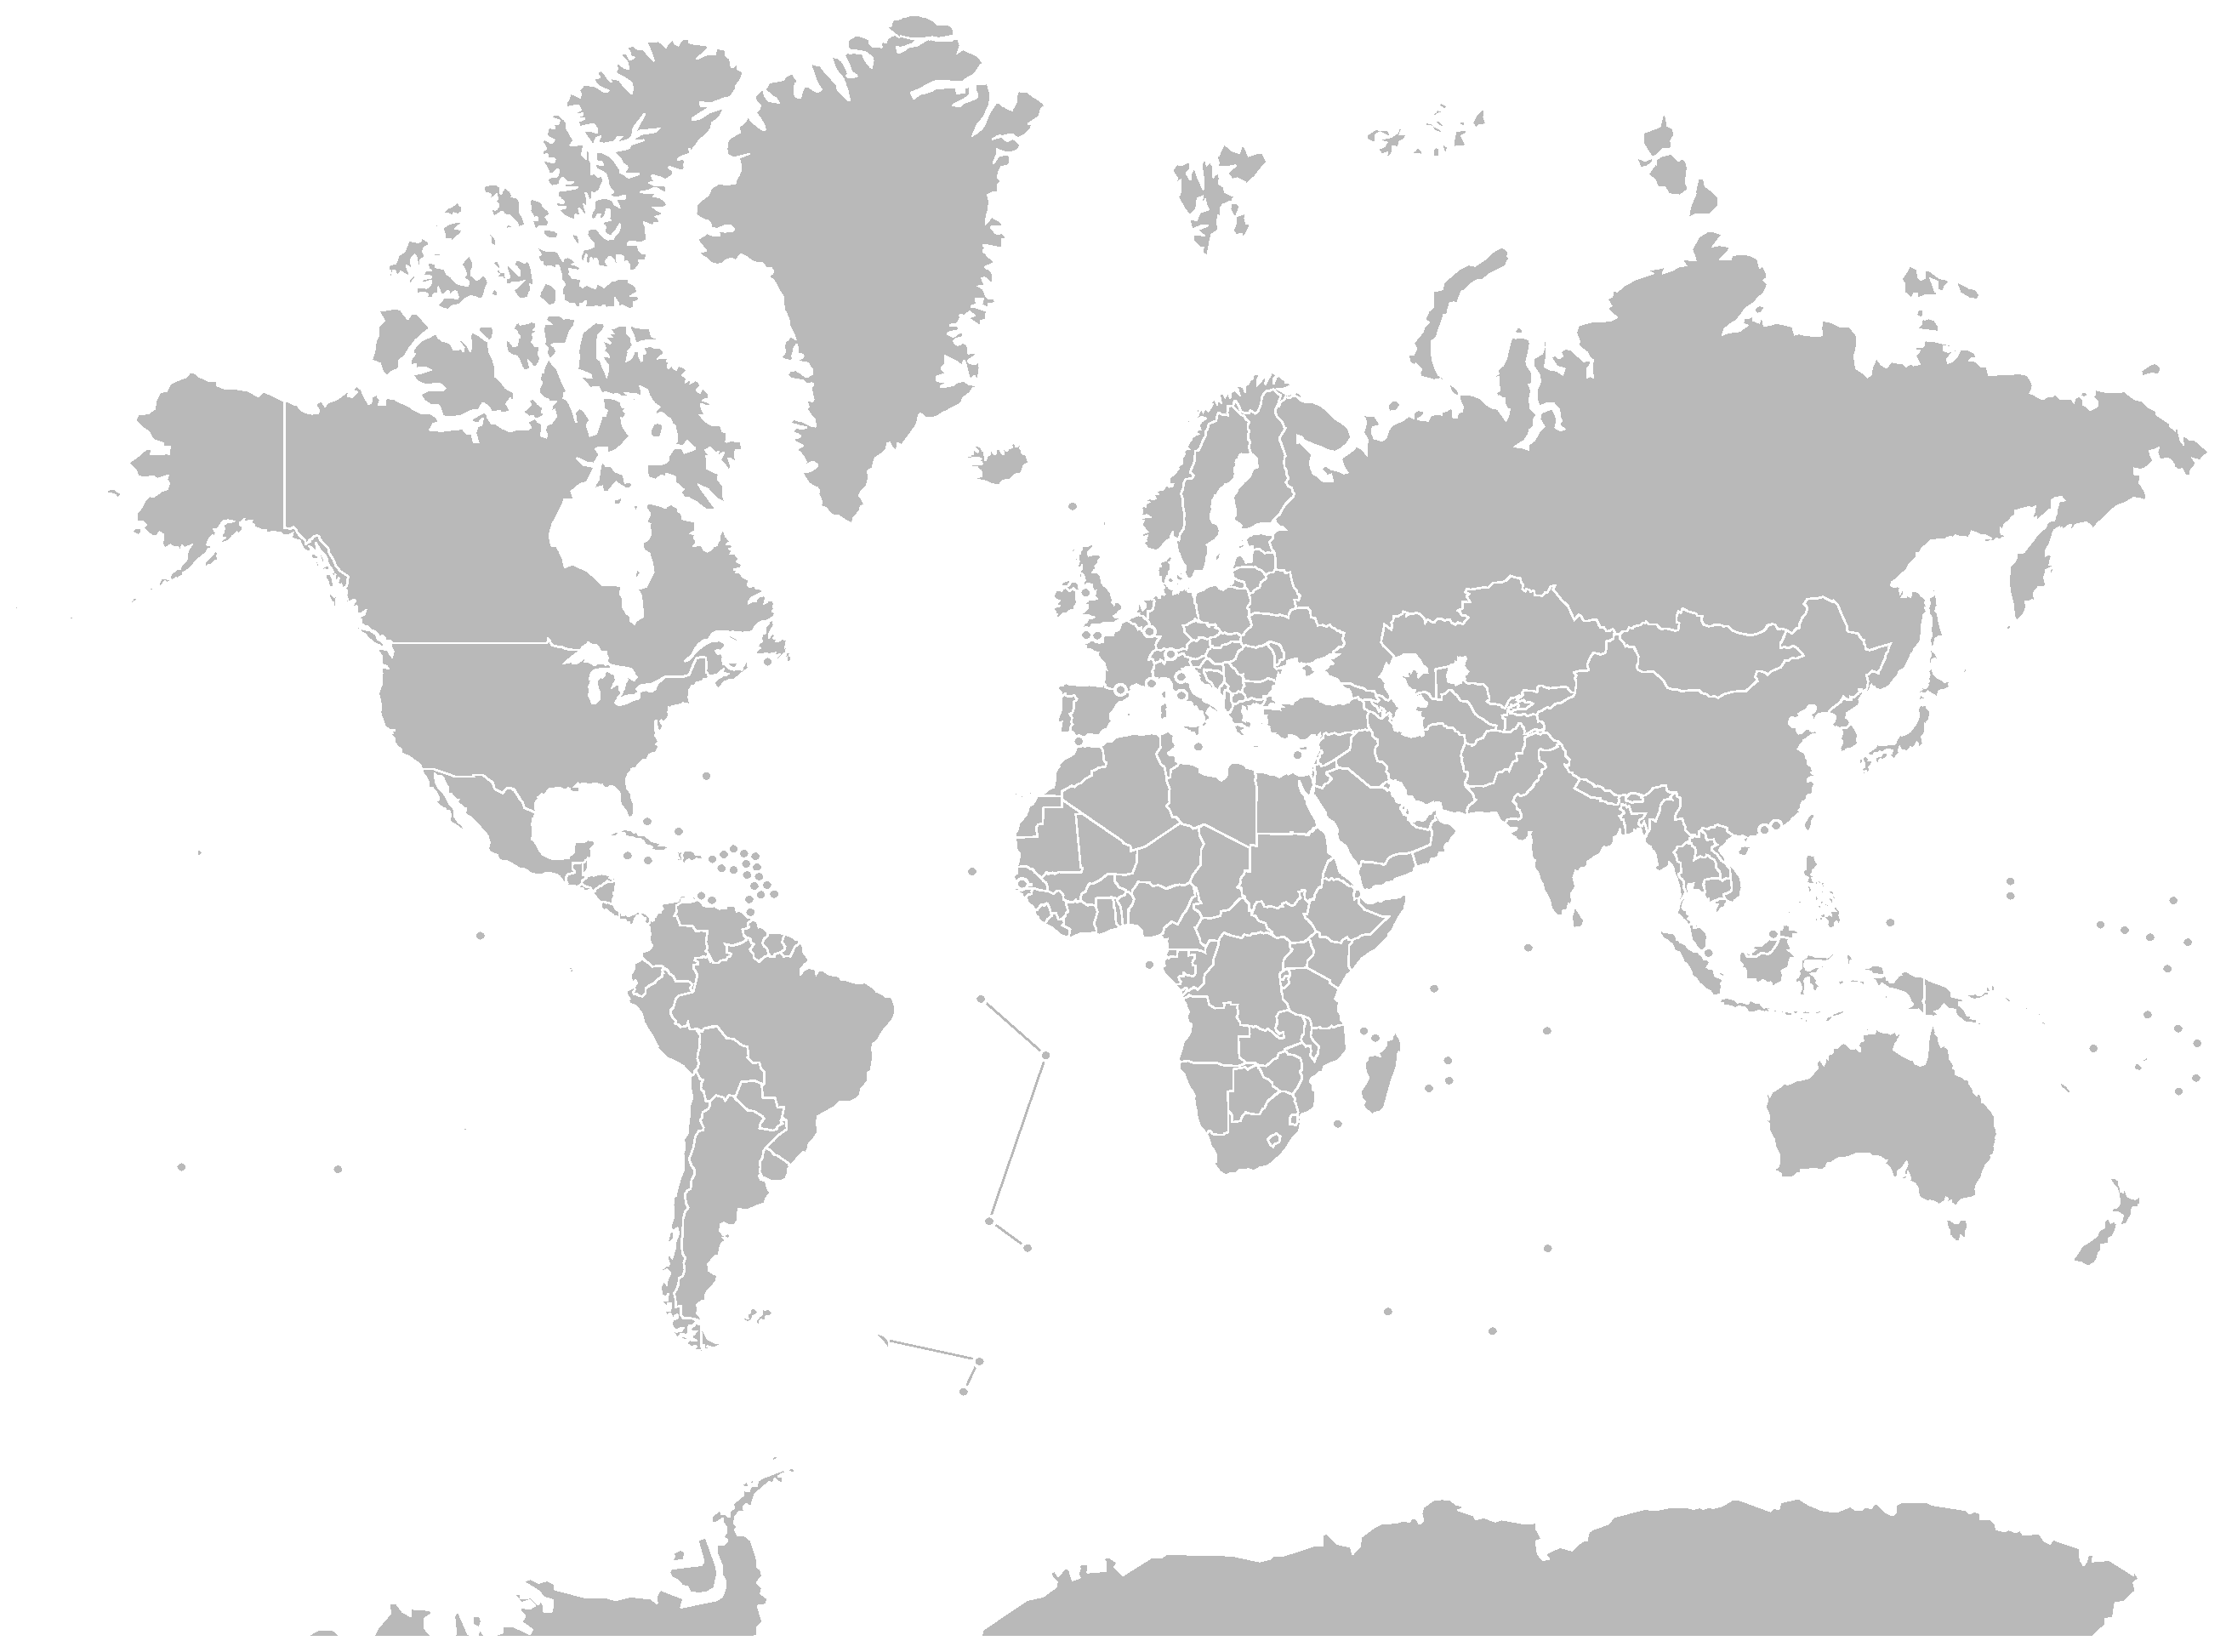
\includegraphics[scale=0.15]{eps/mercator}
		\caption{No existe el mapa perfecto.}
		\label{fig:mapa}
\end{figure}
	
Es interesante aclarar que sí existen mapas que preservan ángulos. De hecho,
vimos que la proyección estereográfica es una aplicación conforme. También
existen mapas que preservan áreas. 

\begin{example}
	Calculemos los símbolos de Christoffel para la parametrización
	\[
		X(u,v)=(\sigma(u)\cos v,\sigma(u)\sin v,\tau(u))
	\]
	de una superficie de revolución. Vimos que
	\[
		E(u,v)=\sigma'(u)^2+\tau'(u)^2,\quad
		F(u,v)=0,\quad
		G(u,v)=\sigma^2(u).
	\]
	De las fórmulas~\eqref{eq:gamma1}--\eqref{eq:gamma6} obtenemos entonces 
	\[
		\Gamma_{11}^1=\frac{\sigma'\sigma''+\tau'\tau''}{\sigma'^2+\tau'^2},\quad
		\Gamma_{11}^2=\Gamma_{12}^1=\Gamma_{22}^2=0,\quad
		\Gamma_{22}^1=\frac{-\sigma\sigma'}{\sigma'^2+\tau'^2},\quad
		\Gamma_{12}^2=\frac{\sigma'}{\sigma}.
	\]
\end{example}

Veamos que el recíproco del teorema de Gauss no es cierto. Para eso
presentaremos dos superficies no localmente isométricas que en todos sus puntos
poseen la misma curvatura gaussiana. 

\begin{example}
	\index{Superficie!de revolución}
	\index{Helicoide}
	Consideremos la superficie $S$ de revolución que se obtiene al rotar la
	curva
	$\sigma(u)=u$, $\tau(u)=\log u$, 
	alrededor del eje $z$ tal como hicimos en el ejemplo~\ref{exa:revolucion}. 
	Si $U=(0,2\pi)\times(0,+\infty)$ y $X\colon U\to\R^3$ es la parametrización
	\[
		X(u,v)=(u\cos v,u\sin v,\log u),
	\]
	el abierto $X(U)\subseteq S$ es también una superficie.  Podemos ver un
	gráfico de esta superficie en la figura~\ref{fig:egregium}. 
	\begin{figure}
		\centering
    	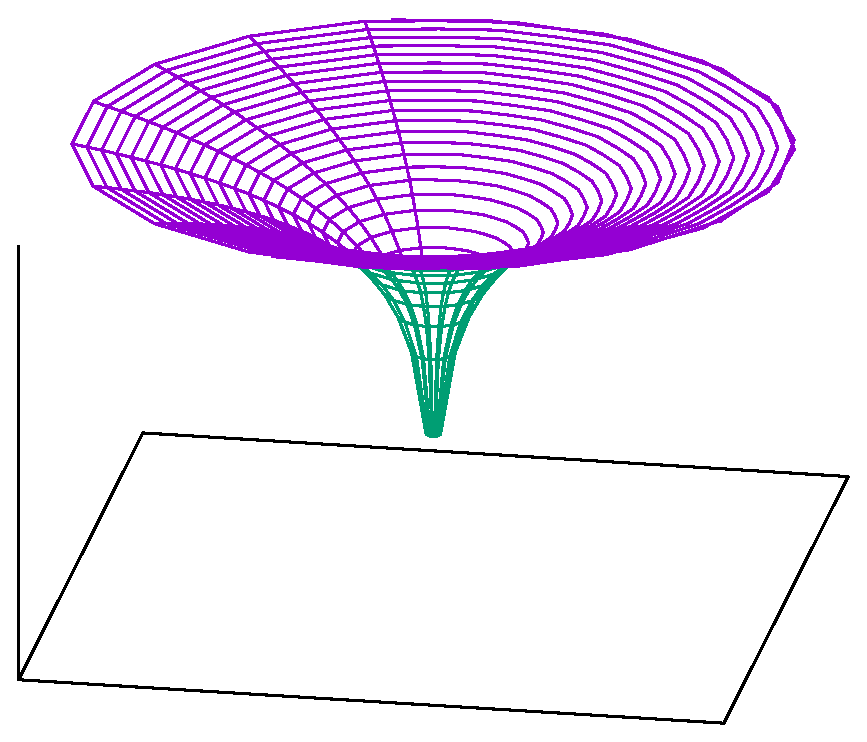
\includegraphics[scale=0.3]{eps/revolucion}
		\caption{Una superficie de revolución.}
		\label{fig:egregium}
	\end{figure}
	Como 
	\[
		\sigma'(u)=1,\quad
		\sigma''(u)=0,\quad
		\tau'(u)=1/u,\quad
		\tau''(u)=-1/u^2,
	\]
	los coeficientes de la primera forma fundamental son:
	\[
		E=1+\frac{1}{u^2},\quad
		F=0,\quad
		G=u^2,
	\]
	y la curvatura gaussiana queda
	\[
		K_X\circ X(u,v)=\frac{-1}{(1+u^2)^2}.
	\]

	Consideremos ahora la superficie $Y(U)$ contenida en el helicoide $T$ que
	vimos en el ejemplo~\ref{exa:helicoide}, donde 
	\[
	Y(u,v)=(u\cos v,u\sin v,v).
	\]
	La primera forma fundamental está entonces dada por
	\[
		E=1+u^2,\quad
		F=0,\quad
		G=1,
	\]
	y curvatura gaussiana igual a 
	\[	
		K_Y\circ Y(u,v)=\frac{-1}{(1+u^2)^2}.
	\]

	A pesar de que las curvaturas gaussianas coinciden, las
	superficies $X(u)$ y $Y(U)$ no son localmente isométricas. De hecho, si
	$f\colon X(U)\to Y(U)$ es una isometría local, entonces, por el
	lema~\ref{lem:isometria_local}, llevaría 
	un punto $X(u,v)$ en un punto de la forma $Y(\pm u,\overline{v})$, una contradicción.
		

	El código utilizado para producir la figura~\ref{fig:egregium} es el
	siguiente:
\begin{lstlisting}
gnuplot> set parametric
gnuplot> set isosamples 50,30
gnuplot> set hidden3d
gnuplot> unset xtics
gnuplot> unset ytics
gnuplot> unset ztics
gnuplot> set key off
gnuplot> set view 60,190
gnuplot> splot u*cos(v),u*sin(v),log(u)
\end{lstlisting}

\end{example}
\chapter{Geodésicas}

\begin{definition}
	\index{Geodésica}
	Sea $S$ una superficie. 
	Diremos que una curva $\gamma$ en $S$ es una \textbf{geodésica} si
	$\langle\gamma''(t),T_{\gamma(t)}S\rangle=0$ para todo $t$.
\end{definition}

Veamos algunas propiedades básicas de las curvas geodésicas:

\begin{proposition}
	Si $\gamma$ es una geodésica, entonces $\|\gamma'(t)\|$ es constante. 
\end{proposition}

\begin{proof}
	Simplemente calculamos
	\[
		\frac{d}{dt}\|\gamma'(t)\|^2=\frac{d}{dt}\langle \gamma'(t),\gamma'(t)\rangle=2\langle \gamma''(t),\gamma'(t)\rangle=0,
	\]
	y en consecuencia $\|\gamma'(t)\|$ es una constante.
\end{proof}

\begin{proposition}
	Si $\gamma$ una curva en $S$ parametrizada por longitud de arco. Entonces
	$\gamma$ es una geodésica si y sólo si $\kappa_g=0$.
\end{proposition}

\begin{proof}
	Sea $X$ una parametrización de $S$. Supongamos primero que $\gamma$ es una
	geodésica. Como entonces $\gamma''$ es paralelo a $N_X$, entonces
	$\kappa_g=\langle\gamma'',N_X\times\gamma'\rangle=0$. Supongamos ahora que
	$\kappa_g=0$. Como entonces $\gamma''$ es perpendicular a
	$N_X\times\gamma'$ y $\{\gamma',N_X,N_X\times\gamma'\}$ es una base de
	$\R^3$, se concluye que $\gamma''$ es paralelo a $N_X$ ya que $\gamma''$ y
	$\gamma'$ son perpendiculares.
\end{proof}

Veamos algunos ejemplos:

\begin{example}
	En el plano, toda parte de una línea recta es una geodésica. 
\end{example}

\begin{example}
	Los grandes círculos de la esfera son geodésicas.
\end{example}

\begin{example}
	La intersección del cilindro $x^2+y^2=1$ con el plano $z=0$ es una geodésica.
\end{example}

\begin{theorem}
	\label{thm:geodesicas}
	Sea $X\colon U\to S$ una parametrización de una superficie $S$ y sea
	$\gamma$ una curva en $X(U)$. Entonces $\gamma$ es una geodésica si y sólo
	si 
	\begin{align*}
			&\frac{d}{dt}(Eu'+Fv')=\frac12(E_uu'^2+2F_uu'v'+G_uv'^2),\\
			&\frac{d}{dt}(Fu'+Gv')=\frac12(E_vu'^2+2F_vu'v'+G_vv'^2).
	\end{align*}
\end{theorem}

\begin{proof}
	La curva $\gamma$ es una geodésica si y sólo si $\gamma''\perp X_u$ y $\gamma''\perp X_v$. Como además 
	$\gamma'=X_uu'+X_vv'$, tenemos entonces que $\gamma$ es una geodésica si y sólo si 
	\[
		\left\langle\frac{d}{dt}(X_uu'+X_vv'),X_u\right\rangle=\left\langle\frac{d}{dt}(X_uu'+X_vv'),X_v\right\rangle=0.
	\]
	Calculamos ahora
	\begin{align*}
		\frac{d}{dt}\langle& X_uu'+X_vv',X_u\rangle-\langle X_uu'+X_vv',\frac{d}{dt}X_u\rangle\\
		&=\left\langle\frac{d}{dt}(X_uu'+X_vv'),X_u\right\rangle\\
		&=\frac{d}{dt}\langle (Eu'+Fv')-\langle X_uu'+x_vv',u'X_{uu}+v'X_{uv}\rangle\\
		&=\frac{d}{dt}(Eu'+Fv')-u'^2\langle X_u,X_{uu}\rangle-u'v'(\langle X_u,X_{uv}\rangle+\langle X_v+X_{uu}\rangle)-v'^2\langle X_v,X_{uv}\rangle.
	\end{align*}
	Como además
	\begin{align*}
		&\frac12 E_u=\langle X_u,X_{uu}\rangle,\\
		&\frac12 G_u=\langle X_v,X_{uv}\rangle,\\
		&F_u=\frac{\partial}{\partial u}\langle X_u,X_{v}\rangle=\langle X_{uu},X_v\rangle+\langle X_u,X_{uv}\rangle,
	\end{align*}
	se concluye diractamente que
	\begin{align*}
		\left\langle\frac{d}{dt}(X_uu'+X_vv'),X_u\right\rangle
		=\frac{d}{dt}(Eu'+Fv')-\frac12(u'^2+2F_uu'v'+v'^2G_u).
	\end{align*}
	La otra fórmula se demuestra de forma similar. 
\end{proof}

Las ecuaciones del teorema anterior quizá no son útiles a la hora de encontrar
geodésicas, ya que estas ecuaciones son en general muy difíciles de resolver.
El punto es que nos permiten obtener el siguiente resultado:

\begin{corollary}
	Sea $S$ una superficie, sea $p\in S$ y sea $v\in T_pS$ un vector unitario.
	Entonces existe una única geodésica $\gamma$ en $S$ parametrizada por
	longitud de arco tal que $\gamma(0)=p$ y $\gamma'(0)=v$. 
\end{corollary}

\begin{proof}
	Las ecuaciones del teorema anterior pueden escribirse como
	\begin{equation}
		\label{eq:geodesicasFG}
		u''=F(u,v,u',v'),\quad
		v''=G(u,v,u',v'),
	\end{equation}
	donde $F$ y $G$ son funciones diferenciables. Si $a,b,c,d\in\R$, la teoría
	de ecuaciones diferenciales nos dice que el sistema~\eqref{eq:geodesicasFG}
	tiene una única solución $(u,v)$ que cumple que $u(0)=a$, $v(0)=b$, $u'(0)=c$,
	$v'(0)=d$ y tal que $u$ y $v$ son funciones diferenciables en algún entorno
	de $t=0$. Sea $X$ una parametrización de $S$ y supongamos que $p=X(a,b)$. 
	Sea $v=cX_u+dX_v$. Entonces
	$\gamma(t)=X(u(t),v(t))$ es una curva en $S$ tal que $\gamma(0)=X(a,b)=p$ y
	$v=\gamma'(0)=cX_u+dX_v$.
\end{proof}

El corolario anterior nos permite calcular, sin resolver ecuaciones
diferenciales, todas las geodésicas de algunas superficies: 

\begin{example}
	Sabemos que las rectas son geodésicas del plano. Como además  en el plano
	existe una única recta que pasa por un cierto punto dado y tiene una cierta
	dirección del plano dada, no existen otras geodésicas.
\end{example}

\begin{example}
	Sabemos que los grandes círculos son geodésicas de la esfera $S^2$. No
	existen otras geodésicas ya que dado $p\in S^2$ y $v\in T_pS^2$, existe un
	gran círculo que pasa por $p$ y tiene a $v$ como vector tangente en $p$
	(basta tomar la intersección de $S^2$ con el plano que pasa por el origen y
	tiene normal $p\times v$). 
\end{example}

Veamos otra consecuencia:

\begin{corollary}
	Sea $f\colon S\to T$ una isometría local. Si $\gamma$ es una geodésica en $S$, entonces
	$f\circ\gamma$ es una geodésica en $T$.
\end{corollary}

\begin{proof}
	Sea $X$ una parametrización de $S$ y sea $p=X(q)\in S$. Si $\gamma$ es una
	geodésica, podemos escribir $\gamma(t)=X(u(t),v(t))$, donde $u(t)$ y $v(t)$
	son funciones diferenciables que satisfacen las ecuaciones del
	teorema~\ref{thm:geodesicas}. Como $Y=f\circ X$ es una parametrización de
	$T$ con la misma forma fundamental que tiene la parametrización $X$, la
	curva $f(\gamma(t))=f(X(u(t),v(t))=Y(u(t),v(t))$ también resulta una
	geodésica en $T$ gracias al teorema~\ref{thm:geodesicas}.
\end{proof}

% FIXME: agregar superficies de revolución

Veamos ahora cuál es la conexión entre las curvas geodésicas y las curvas de
menor longitud que unen dos ciertos puntos de una superficie.  
Antes necesitamos una lema:

\begin{lemma}
	\label{lem:suavizante}
	Existe una función diferenciable $\phi$ tal que $\psi(t)>0$ si $t\in(t_0-\eta,t_0+\eta)$
	y $\psi(t)=0$ si $t\not\in(t_0-\eta,t_0+\eta)$. 
\end{lemma}

\begin{proof}
	Primero observamos que, como 
	\[
		\lim_{t\to 0}t^ne^{1/t^2}=0
	\]
	para todo $n\in\N$, la función
	\[
		\theta(t)=\begin{cases}
			e^{-1/t^2} & \text{si $t\geq0$},\\
			0 & \text{si $t<0$},
		\end{cases}
	\]
	es diferenciable. La función 
	$\psi(t)=\theta(1+t)\theta(1-t)$ 
	es también diferenciable y cumple que $\psi(t)>0$ si $t\in (-1,1)$ y $\psi(t)<0$ si $t\not\in(-1,1)$. La función
	\[
		\phi(t)=\psi\left(\frac{t-t_0}{\eta}\right)
	\]
	es entonces diferenciable y cumple con las condiciones del enunciado.
\end{proof}


Sea $X\colon
U\to X(U)$ una parametrización de una superficie $S$ y sean $p,q\in X(U)$ dos
puntos tales que $p\ne q$. Sea $\gamma$ una curva parametrizada por longitud de
arco que pasa por $p$ y por $q$. Si $\gamma$ es el camino más corto entre $p$ y
$q$, podemos pensar que $\gamma$ es en realidad una de las curvas de una
familia diferenciable de curvas del parche $X(U)$ que pasan por $p$ y $q$. Para
definir esa familia diferenciable de curvas hacemos lo siguiente: Para cada
$\tau\in(-1,1)$ tenemos una curva $\gamma_\tau$ en el parche $X(U)$ y se
verifican las siguientes propiedades:
\begin{enumerate}
	\item cada $\gamma_\tau(t)$ está definida para $t\in (-1,1)$, 
	\item existen $a,b\in\R$ con $-1<a<b<1$ y tales que $\gamma_{\tau}(a)=p$ y $\gamma_{\tau}(b)=q$,
	\item la función $(-1,1)\times(-1,1)\to\R^3$, $(\tau,t)\mapsto\gamma_{\tau}(t)$, es diferenciable, y por último
	\item $\gamma_0=\gamma$.
\end{enumerate}
Tenemos entonces definida una familia diferenciable
$\{\gamma_{\tau}:\tau\in(-1,1)\}$ de curvas en $X(U)$. La longitud de cada
$\gamma_{\tau}$ entre $p$ y $q$ será denotada por
\[
	L(\tau)=\int_a^b\|\gamma_{\tau}'(t)\|dt.
\]

Observemos que no suponemos que las curvas $\gamma_{\tau}$ están parametrizadas
por longitud de arco. 

\begin{theorem}
	Sea $\gamma$ una curva parametrizada por longitud de arco. Entonces
	$\gamma$ es una geodésica si y sólo si 
	\[
		\frac{d}{d\tau}\Big|_{\tau=0}L(\tau)=0.
	\]
\end{theorem}

\begin{proof}
	Como las funciones involucradas son diferenciables, podemos intercambiar el
	orden de las derivadas con el de la integral. Si $g(\tau,t)=\|\gamma_{\tau}'(t)\|$, entonces 
	\begin{align*}
		\frac{d}{d\tau}L(\tau)
		&=\frac{d}{d\tau}\int_a^b\|\gamma_{\tau}'(t)\|dt
		=\int_a^b\frac{\partial}{\partial\tau}\sqrt{g(\tau,t)}dt
		=\frac12\int_a^bg(\tau,t)^{-1/2}\frac{\partial g}{\partial\tau}dt.
	\end{align*}
	Observemos que, como 
	\[
		g(\tau,t)=Eu'^2+2Fu'v'+Gv'^2,
	\]
	entonces un cálculo tedioso nos dice que
	\begin{align*}
		\frac{\partial g}{\partial\tau} &= \dots
	\end{align*}
	Luego podemos escribir 
	\begin{align*}
		&\frac{d}{d\tau}L(\tau)=\int_a^b \left(U\frac{\partial u}{\partial\tau}+V\frac{\partial v}{\partial\tau}\right)dt,
		\shortintertext{donde}
		&U=\frac12g^{-1/2}(E_uu'^2+2F_uu'v'+G_uv'^2)-\frac{d}{dt}(g^{-1/2}(Eu'+Fv')),\\
		&V=\frac12g^{-1/2}(E_vu'^2+2F_vu'v'+G_vv'^2)-\frac{d}{dt}(g^{-1/2}(Fu'+Gv')).
	\end{align*}
	Como $\|\gamma'(t)\|^2=1$ para todo $t\in(-1,1)$, entonces 
	$g(0,t)=1$ para todo $t\in(-1,1)$. 

	Si $\gamma$ es una geodésica, entonces $U=V=0$ si $\tau=0$ y luego 
	\[
		\frac{d}{d\tau}\Big|_{\tau=0}L(\tau)=0.
	\]

	Supongamos entonces que 
	\[
		\int_a^b=0 
	\]
	si $\tau=0$. Si $U(0,t)\ne0$, entonces podemos suponer sin perder
	generalidad que existe $t_0\in(a,b)$ tal que $U(0,t_0)>0$ (ya que el caso
	en que $U(0,t_0)<0$ se hace de forma similar). Como $U$ es continua, existe
	$\eta>0$ tal que $U(0,t)>0$ para todo $t\in(t_0-\eta,t_0+\eta)$. Sea $\phi$
	una función diferenciable tal que $\phi(t)>0$ si $t\in (t_0-\eta,t_0+\eta)$
	y $\phi(t)=0$ en otro caso (la existencia de una tal $\phi$ está
	garantizada por el lema~\ref{lem:suavizante}). Sean 
	\[
		\gamma(t)=X(u(t),v(t)),\quad
		\gamma_{\tau}(t)=X(u(\tau,t),v(\tau,t)),
	\]
	donde 
	\[
		u(\tau,t)=u(t)+\tau\phi(t),\quad
		v(\tau,t)=v(t).
	\]
	Como $\partial u/\partial\tau=\phi$ y $\partial v/\partial\tau=0$ para todo $\tau$ y todo $t$, tenemos que
	\[
		0=\int_a^b(\dots)dt\Big|_{\tau=0}=\int_{t_0-\eta}^{t_0+\eta}U(0,t)\phi(t)dt>0,
	\]
	una contradicción. Similarmente vemos que $V(0,t)=0$ para todo $t\in(a,b)$.
	Luego $\gamma$ es una geodésica pues satisface las ecuaciones geodésicas.
\end{proof}

Veamos algunas consecuencias importantes del teorema anterior. La primera es la
siguiente: 
\begin{enumerate}
	\item El camino más corto entre dos puntos de una superficie es una
		geodésica. En efecto, si $\gamma$ es el camino más corto en un
		parche $X(U)$ entre los puntos $p$ y $q$, entonces la función $L(\tau)$
		del teorema anterior tendrá un mínimo absoluto cuando $\tau=0$. Luego
		$\frac{d}{d\tau}L(\tau)=0$ si $\tau=0$ y entonces, por el teorema
		anterior, $\gamma$ será una geodésica. 
	\item Una geodésica no siempre será el camino más corto entre dos puntos. 
		Si $\gamma$ es una geodésica que une los puntos $p$ y $q$, entonces
		$L(\tau)$ tendrá un punto crítico en $\tau=0$. Sin embargo, como bien
		sabemos gracias al curso de cálculo, esto no implica la existencia de
		un mínimo ahí. 
	\item El camino más corto entre dos puntos de una superficie podría no existir. Parece raro esto, pero
		pensemos en el plano $z=0$ sin el oriden de coordenadas. Es una superficie (porque es un abierto contenido en una superficie) 
		pero el camino más corto que une $p=(-1,0,0)$ con $q=(1,0,0)$ no pertenece a la superficie (y puede demostrarse
		que no existe otro camino más corto entre $p$ y $q$).


\end{enumerate}

%Cualquier animal que vive sobre una esfera y viajara con velocidad constante alrededor del ecuador creería que su velocidad  

\index{Campo vectorial tangente!a lo largo de una curva}
Sea $\gamma$ una curva en una superficie $S$. Un \textbf{campo vectorial
tangente a lo largo de $\gamma$} es una función diferenciable $(0,1)\to\R^3$
tal que $v(t)\in T_{\gamma(t)}S$ para todo $t\in(0,1)$. La \textbf{derivada
covariante} $\nabla_\gamma v$ de $v$ al lo largo de $\gamma$ se define como la proyección ortogonal 
de $v'$ en $T_{\gamma(t)}S$, es decir
\[
	\nabla_{\gamma}v=v'-\langle v',N\rangle N,
\]
donde $N$ es el vector normal unitario de $T_{\gamma(t)}S$. Diremos que el
campo $v$ es \textbf{paralelo} a lo largo de $\gamma$ si $\nabla_{\gamma}v=0$.

\begin{proposition}
	El campo $v$ es paralelo a lo largo de $\gamma$ si y sólo si $v'\perp
	T_{\gamma(t)}S$.
\end{proposition}

\begin{proof}
	Si $v$ es paralelo a lo largo de $\gamma$, entonces, por definición,
	$\nabla_{\gamma}v=0$. Luego $v'=\langle v',N\rangle N$ y entones $v'\perp
	T_{\gamma(t)}S$. Recíprocamente, si $v'\perp T_{\gamma(t)}S$, entonces
	$v'=\lambda N$ para algún $\lambda\in\R$ y luego
	\[
		\nabla_{\gamma}v=v'-\langle v',N\rangle N=v'-\langle \lambda N,N\rangle N=v'-\lambda N=0.\qedhere
	\]
\end{proof}

\begin{proposition}
	Sea $\gamma(t)=X(u(t),v(t))$ una curva en el parche $X(U)$ de $S$. Sean
	$\alpha$ y $\beta$ funciones diferenciables tales que
	$v(t)=\alpha(t)X_u+\beta(t)X_v$ es un campo vectorial tangente a lo largo
	de $\gamma$. Entonces $v$ es paralelo a lo largo de $\gamma$ si y sólo si 
	\begin{align*}
		&\alpha'+(\Gamma_{11}^1 u'+\Gamma_{12}^1v')\alpha+(\Gamma_{12}^1u'+\Gamma_{22}^1v')\beta=0,\\
		&\beta'+(\Gamma_{11}^2 u'+\Gamma_{12}^1v')\alpha+(\Gamma_{12}^2u'+\Gamma_{22}^2v')\beta=0.
	\end{align*}
\end{proposition}

\begin{proof}
	Ya calculamos:
	\begin{align*}
		X_{uu}=\Gamma_{11}^1 X_u+\Gamma_{11}^2X_v+eN_X,\\
		X_{uv}=\Gamma_{12}^1 X_u+\Gamma_{12}^2X_v+fN_X,\\
		X_{vv}=\Gamma_{22}^1 X_u+\Gamma_{22}^2X_v+gN_X.
	\end{align*}
	Entonces, como
	\[
		v'=\alpha'X_u+\beta'X_v+\alpha u'X_{uu}+\alpha(X_{uu}u'+X_{uv}v')+\beta(X_{uv}u'+X_{vv}v')
	\]
	se concluye que	
	\begin{multline}
		\label{eq:X_uX_v=0}
		v'=\alpha'X_u+\beta'X_v+\alpha u'(\Gamma_{11}^1X_u+\Gamma_{11}^2X_v+eN_X)\\
		+(\alpha v'+\beta u')(\Gamma_{12}^1X_u+\Gamma_{12}^2X_v+fN_X)
		+\beta v'(\Gamma_{22}^1X_u+\Gamma_{22}^2X_v+gN_X).
	\end{multline}
	Sabemos que $v$ es paralelo a lo largo de $\gamma$ si y sólo si $v'$ es
	paralelo a $N_X$. Esto es equivalente a pedir que los coeficientes de $X_u$
	y $X_v$ en la expresión~\eqref{eq:X_uX_v=0} sean ambos iguales de cero. 
\end{proof}

El sistema de ecuaciones del 
resultado anterior puede escribirse
como
\[
	\alpha'=F(\alpha,\beta,t),\quad
	\beta'=G(\alpha,\beta,t),
\]
donde $F$ y $G$ son funciones diferenciables. Dado cualquier conjunto de
condiciones iniciales, este sistema tiene una única solución. Es decir: si
$\alpha_0,\beta_0\in\R$, entonces existen únicas funciones diferenciables
$\alpha$ y  $\beta$ tales que $\alpha'=F(\alpha,\beta,t)$,
$\beta'=G(\alpha,\beta,t)$, $\alpha(t_0)=\alpha_0$ y $\beta(t_0)=\beta_0$. Luego 
dada una curva $\gamma$ en $S$ y un vector $v_0\in T_{\gamma(t_0)}S$, existe un 
único campo vectorial $v$ que cumple que $v(t_0)=v_0$ y además 
es paralelo a lo largo de $\gamma$.

\begin{corollary}
	Una curva $\gamma$ en una superficie $S$ es una geodésica si y sólo si para
	todo pedazo $\gamma(t)=X(u(t),v(t))$ de $\gamma$ contenido en un parche $X$, se satisface 
	el siguiente sistema de ecuaciones:
	\begin{align*}
		&u''+\Gamma_{11}^1u'^2+2\Gamma_{12}^1u'v'+\Gamma_{22}^1v'=0,\\
		&u''+\Gamma_{11}^2u'^2+2\Gamma_{12}^2u'v'+\Gamma_{22}^2v'=0.
	\end{align*}
\end{corollary}

\begin{proof}
	Primero observamos que, por definición, una curva $\gamma$ es una geodésica si y sólo si $\gamma'$ es paralelo
	a lo largo de $\gamma$. Como $\gamma'=u'X_u+v'X_v$ por la regla de la
	cadena, las ecuaciones geodésicas son exactamente las ecuaciones del
	enunciado, donde $\alpha=u'$ y $\beta=v'$.
\end{proof}


\chapter{El teorema de Gauss--Bonnet}

En esta sección vamos a demostrar varias versiones del famoso teorema de
Gauss-Bonnet. Primero haremos un repaso de la teoría de curvas planas.

\index{Curvatura!con signo}
Sea $\gamma$ una curva plana parametrizada por longitud de arco. Sea
$T=\gamma'$ el vector tangente a $\gamma$ y sea $N$ el vector unitario normal
obtenido al rotar $T$ en sentido antihorario en un ángulo $\pi/2$. Como
$T'=\gamma''$ y $T=\gamma'$ son perpendiculares, el vector $T'$ es paralelo a
$N$ y luego puede escribirse $\gamma''=\kappa_s N$ para alguna función
$\kappa_s$. La función $\kappa_s$ se conoce como \textbf{curvatura con signo}
de $\gamma$. Como por construcción $\|N\|=1$, sabemos que la curvatura usual $\kappa$ 
satisface 
\[
	\kappa=\|\gamma''\|=\|\kappa_s N\|=|\kappa_s|.
\]

\begin{proposition}
	Sea $\gamma\colon (a,b)\to\R^2$ una curva parametrizada por longitud de arco. Para $s_0\in (a,b)$ sea
	$\varphi_0$ tal que $\gamma'(s_0)=(\cos\varphi_0,\sin\varphi_0)$. Existe entonces una única función 
	$\varphi\colon (a,b)\to\R$ diferenciable tal que $\varphi(s_0)=\varphi_0$ y tal que 
	\[
		\gamma'(s)=(\cos\varphi(s),\sin\varphi(s))
	\]
	para todo $s\in (a,b)$. 
\end{proposition}

\begin{proof}
	Como $\gamma$ está parametrizada por longitud de arco, podemos escribir 
	$\gamma'(s)=(\sigma(s),\tau(s))$, donde $\sigma(s)^2+\tau(s)^2=1$ para todo $s\in(a,b)$. Sea
	\[
		\varphi(s)=\varphi_0+\int_{s_0}^s(\sigma\tau'-\tau\sigma')(t)dt.
	\]
	Entonces $\varphi(s_0)=\varphi_0$ y además, como $\sigma$ y $\tau$ son
	diferenciables, $\varphi$ es una función diferenciable. 

	Sean $F=\sigma\cos\varphi+\tau\sin\varphi$ y 
	$G=\sigma\sin\varphi-\tau\cos\varphi$. 
	Entonces 
	\[
		F'=(\sigma'+\tau\varphi')\cos\varphi+(\tau'-\sigma\varphi')\sin\varphi
	\]
	y luego
	\begin{align*}
		&\sigma'+\tau\varphi'=\sigma'(1-\tau^2)+\sigma\tau\tau'=\sigma(\sigma\sigma'+\tau\tau')=0,\\
		&\tau'-\sigma\varphi'=0.
	\end{align*}
	Esto implica que $F'=0$ y luego $F$ es constante. Análogamente se demuestra que $G$ es una función constante.
	\dots

	
	Similarmente se demuestra que la función 
\end{proof}
\chapter{Ejercicios}

\begin{exercise}
	Demuestre que si $S$ es una superficie, $S$ es un conjunto abierto.
\end{exercise}

\begin{exercise}
	Calcula las curvaturas en el punto $p=(0,0,0)$ de la superficie dada por
	$z=x^2+ky^2$, donde $k$ es una constante positiva.
\end{exercise}

\begin{exercise}
	Calcule los coeficientes de la primera forma fundamental del plano $z=0$ en
	coordenadas polares.
\end{exercise}
	
